\chapter{Technologies et réalisation}

Ce chapitre décrit l'ensemble des technologies, outils et méthodes qui ont été utilisés pour la mise en œuvre du projet. Il présente d'abord les choix techniques, puis détaille l'environnement de déploiement, l'implémentation du système (structure du code et interfaces utilisateur), ainsi que la stratégie de tests appliquée. Enfin, une conclusion synthétique fait le point sur les réalisations et les éventuelles difficultés rencontrées.

%%%%%%%%%%%%%%%%%%%%%%%%%%%%%%%%%%%%%%%%%%%%%%%%%%%%%%%%%%%
\section{Introduction}
%%%%%%%%%%%%%%%%%%%%%%%%%%%%%%%%%%%%%%%%%%%%%%%%%%%%%%%%%%%
Dans cette section introductive, l'objectif est de donner une vue d'ensemble des aspects techniques et pratiques abordés dans ce chapitre. Nous y expliquons notamment :
\begin{itemize}
    \item \textbf{Les choix technologiques :} Justification des outils et frameworks sélectionnés en fonction des besoins fonctionnels (scalabilité, sécurité) et des contraintes techniques du projet.
    \item \textbf{L'environnement de déploiement :} La manière dont l'infrastructure est configurée, notamment via la conteneurisation, pour supporter l'écosystème microservices.
    \item \textbf{L'implémentation et l'interface utilisateur :} Les détails sur la structuration du code source (backend et frontend) et la conception ergonomique des interfaces.
    \item \textbf{La stratégie de validation :} La méthodologie adoptée pour tester le système et garantir sa conformité aux exigences initiales.
\end{itemize}

Cette partie prépare le lecteur à comprendre comment les décisions prises au niveau de la conception se traduisent concrètement lors de la réalisation technique de la plateforme Certif-fun.

%%%%%%%%%%%%%%%%%%%%%%%%%%%%%%%%%%%%%%%%%%%%%%%%%%%%%%%%%%%
\section{Choix techniques et outils}
%%%%%%%%%%%%%%%%%%%%%%%%%%%%%%%%%%%%%%%%%%%%%%%%%%%%%%%%%%%
La sélection de la pile technologique pour \textbf{Certif-fun} n'est pas fortuite ; elle résulte d'une analyse comparative visant à concilier réactivité, sécurité et modularité.

\subsection{Langages, Frameworks et Bases de données}
Cette sous-section détaille l'ensemble des piliers technologiques et outils d'infrastructure sur lesquels repose l'ossature de la plateforme \textbf{Certif-fun} :

\begin{itemize}
    \item \textbf{Framework Backend (Java/Spring Boot) :}  
    Spring Boot a été choisi pour orchestrer la coordination entre nos différents microservices (Admin, Formateur, Apprenant) grâce à sa configuration simplifiée \cite{bairstow2023spring}. Son architecture basée sur l’Inversion de Contrôle (IoC) assure un couplage faible entre les modules, facilitant grandement la maintenance du système. Pour la sécurité, nous avons intégré Spring Security afin de gérer rigoureusement l’authentification via des jetons JWT.
    
    \item \textbf{Framework Frontend (React \& Tailwind CSS) :}  
    React permet de construire des interfaces utilisateur interactives basées sur des composants réutilisables et une gestion efficace du Virtual DOM \cite{minnick2022foundation}. Ce choix est indispensable pour rafraîchir les vues instantanément et afficher en temps réel les alertes de surveillance ou les indicateurs de session. Nous l’avons associé à Tailwind CSS dont l’approche utilitaire offre une grande liberté pour concevoir une interface moderne et adaptable.
    
    \item \textbf{Intelligence Artificielle (Python/FastAPI \& YOLOv8) :}  
    YOLOv8 assure la détection d’objets en temps réel pour identifier l’utilisation de téléphones ou la présence de plusieurs personnes \cite{sohan2025review}. FastAPI expose ces capacités via des API hautes performances, facilitant la validation automatique des données et la génération de documentation \cite{fastapi_docs}. Enfin, MediaPipe est intégré pour construire des pipelines de perception multimédia dédiés au suivi précis des visages et des poses \cite{lugaresi2019mediapipe}.
    
    \item \textbf{Visioconférence (LiveKit \& WebRTC) :}  
    Nous utilisons les normes WebRTC pour permettre une communication audio et vidéo fluide directement dans le navigateur sans nécessiter de plugins \cite{romano2012webrtc}. LiveKit s’appuie sur une architecture SFU (Selective Forwarding Unit) qui transfère la charge du routage des flux médias vers le serveur. Cette approche garantit une stabilité optimale tout en allégeant significativement la consommation CPU du navigateur des apprenants.
    
    \item \textbf{Grands Modèles de Langage (Ollama / Mistral, Llama \& Qwen) :}  
    Ollama facilite le déploiement local des modèles de langage tels que Mistral 7B et Llama 3.2 pour la génération automatique de quiz \cite{novais2025using}. Ce choix délibéré garantit la confidentialité totale des données pédagogiques car aucune information ne transite vers des API externes. Le système produit des réponses structurées en JSON qui sont directement intégrées et exploitées par notre application.
    
    \item \textbf{Orchestration et Conteneurisation (Docker \& Docker Compose) :}  
    L’ensemble des composants de la plateforme a été encapsulé dans des conteneurs Docker pour garantir une cohérence parfaite entre les environnements \cite{ibrahim2021docker}. Docker Compose nous permet de démarrer toute l’infrastructure en une seule commande tout en isolant le réseau interne des services. Cette organisation simplifie le déploiement et assure la portabilité de la solution sur différents serveurs.
    
    \item \textbf{Routage et Proxy Inverse (Nginx) :}
    Nginx joue le rôle de point d’entrée unique pour rediriger efficacement les requêtes vers les services frontends et backends appropriés \cite{reese2008nginx}. Il optimise les performances globales de la plateforme grâce à la compression des ressources et à la distribution intelligente de la charge. En outre, il renforce la sécurité en gérant les règles CORS et en ajustant les limites de taille des requêtes HTTP.
    
    \item \textbf{Gestion de Versions et Collaboration (Git \& GitHub) :}  
    Git a constitué un outil incontournable pour garder une trace précise de l’évolution du code source de chacun de nos microservices. L'hébergement sur GitHub a permis de structurer le développement de façon méthodique grâce à un flux de travail collaboratif efficace. Cette organisation a également facilité la mise en place d'un processus de déploiement plus fluide et mieux contrôlé.
    
    \item \textbf{Persistance des données (PostgreSQL) :}  
    PostgreSQL a été retenu pour sa fiabilité et sa conformité aux propriétés ACID, garantissant l’intégrité des données lors de transactions complexes \cite{google_postgresql}. Nous utilisons Spring Data JPA couplé à Hibernate pour offrir un mapping objet-relationnel performant et sécurisé entre le code et la base de données. Ce choix permet de stocker et d'interroger efficacement l'ensemble des données structurées liées aux certifications.
\end{itemize}

\subsection{Outils de développement et collaboration}
La qualité du code, la rigueur de la modélisation et la fluidité globale du cycle de développement ont été assurées par une sélection rigoureuse d'outils professionnels :

\begin{itemize}
    \item \textbf{Environnements de Développement (IDE) :}  
    Nous avons tiré parti de la complémentarité entre deux éditeurs majeurs pour optimiser notre productivité. VS Code a été utilisé pour le Frontend et la partie IA grâce à sa légèreté et ses extensions spécialisées. IntelliJ IDEA a été réservé au développement des microservices Java pour son support natif exceptionnel de Spring Boot.
    
    \item \textbf{Gestion de Versions et Dépôts (Git \& GitHub) :}  
    Git a été au cœur de la gestion du code source avec une stratégie de branches par fonctionnalité pour un travail parallèle sécurisé. Le dépôt privé sur GitHub a assuré une synchronisation fiable et une sauvegarde continue du projet. Cette organisation a permis de structurer le développement de façon méthodique tout au long du cycle de vie.
    
    \item \textbf{Gestionnaires de Dépendances et de Build (Maven \& NPM/Vite) :}  
    La gestion des dépendances a été segmentée selon la nature des couches applicatives du système. Maven s’est chargé de la compilation et du cycle de vie des microservices Spring Boot. Pour la partie Frontend, nous avons combiné la puissance de NPM pour les paquets et la rapidité de Vite pour le build.
    
    \item \textbf{Serveur d'automatisation (Jenkins) :}
    Jenkins est utilisé comme serveur d’automatisation open-source pour piloter nos pipelines CI/CD \cite{jenkins2015continuous}. Il automatise les étapes critiques de compilation, de test et de génération des artifacts de déploiement. Cette approche garantit une livraison continue stable et réduit les risques d'erreurs humaines.
    
    \item \textbf{Frameworks de Test (JUnit 5 \& pytest) :}
    JUnit 5 est employé pour l'écriture et l'exécution des tests unitaires automatisés au sein de l'écosystème Java \cite{kleuker2019junit5}. Parallèlement, pytest simplifie la validation du code Python dédié aux modules d'intelligence artificielle \cite{pytest_docs}. Cette double couverture assure une robustesse logicielle sur l'ensemble des microservices du projet.
    
    \item \textbf{Tests et Validation d'APIs (Postman \& Newman) :}
    Postman a servi d'interface principale pour le développement et le test unitaire des points de terminaison REST. Newman permet d'automatiser l'exécution de ces collections de tests directement en ligne de commande \cite{postman_newman_docs}. Cette combinaison facilite la validation rigoureuse des échanges de données entre le frontend et le backend.
    
    \item \textbf{Administration de Bases de données (pgAdmin 4) :}  
    pgAdmin 4 a été utilisé comme interface graphique principale pour interagir avec nos bases de données PostgreSQL. Il nous a permis d'inspecter les schémas générés par Hibernate et d'exécuter des scripts SQL de débogage. Cet outil a été essentiel pour surveiller l'intégrité des données tout au long de la phase de réalisation.
    
    \item \textbf{Contrôle et Exécution des LLMs (Ollama CLI) :}  
    La gestion des modèles de langage a été pilotée directement depuis le terminal via l'interface en ligne de commande d'Ollama. Cet outil a permis de configurer les modèles Mistral et Llama 3.2 tout en testant leurs comportements via des invites personnalisées. Il assure une intégration fluide des capacités génératives au sein de notre service de quiz.
    
    \item \textbf{Modélisation et Conception UML (StarUML, Draw.io \& Lucidchart) :}  
    StarUML a été l'outil de référence pour produire les diagrammes structurels et comportementaux conformes aux standards. Draw.io et Lucidchart ont complété cette phase pour l'élaboration de schémas d'architecture plus souples et accessibles. Ces outils ont garantit une documentation technique claire et structurée pour l'ensemble du système.
\end{itemize}

\subsection{Protocoles et bibliothèques de support}
En complément des frameworks majeurs, plusieurs protocoles et bibliothèques spécialisées ont été intégrés pour assurer la fluidité des échanges et la robustesse des fonctionnalités :

\begin{itemize}
    \item \textbf{Communication REST et JSON :} 
    L'intégralité des échanges de données entre les frontends React et les microservices Spring Boot repose sur des API REST. Le format JSON a été privilégié pour sa légèreté et sa compatibilité native avec JavaScript, facilitant le mapping des données complexes.
    
    \item \textbf{Sécurisation via JWT (JSON Web Tokens) :} 
    Pour garantir une architecture \textit{stateless} et sécurisée, nous avons implémenté l'authentification par jetons JWT \cite{mahindrakar2020jwt}. Ce protocole permet de transporter les informations d'identité et les rôles utilisateur de manière cryptée, évitant ainsi le stockage de sessions sur le serveur et facilitant la scalabilité des microservices.
    
    \item \textbf{Axios (Client HTTP) :} 
    Côté frontend, la bibliothèque \textbf{Axios} a été utilisée pour orchestrer les appels asynchrones vers les backends. Elle nous a permis de mettre en place des intercepteurs pour injecter automatiquement le token JWT dans les en-têtes de chaque requête et de gérer de manière centralisée les erreurs HTTP.
    
    \item \textbf{Spring Data JPA et Hibernate :} 
    Pour la couche de persistance, nous avons utilisé Spring Data JPA couplé à Hibernate. Cette approche permet de manipuler les données PostgreSQL sous forme d'objets Java, automatisant ainsi la génération des schémas et garantissant l'intégrité référentielle des données.
    
    \item \textbf{MediaPipe et OpenCV :} 
    Pour le module de proctoring, nous avons couplé YOLOv8 avec les bibliothèques \textbf{MediaPipe} \cite{lugaresi2019mediapipe} et \textbf{OpenCV}. MediaPipe assure le suivi des points de repère faciaux (Landmarks) pour l'analyse du regard, tandis qu'OpenCV gère les flux d'images et les transformations matricielles nécessaires avant l'inférence.
\end{itemize}

%%%%%%%%%%%%%%%%%%%%%%%%%%%%%%%%%%%%%%%%%%%%%%%%%%%%%%%%%%%

\begin{itemize}
    \item \textbf{Processeur (CPU) :} 4 cœurs vCPU virtuels (architecture x86\_64), garantissant un traitement parallèle efficace des requêtes REST, de l'inférence YOLOv8 et de la génération de texte par les modèles de langage.
    \item \textbf{Mémoire Vive (RAM) :} 16 Go de RAM DDR4 ECC, une capacité indispensable pour faire tourner simultanément les trois instances Java/Spring Boot, le serveur d'IA Ollama et la base de données PostgreSQL, sans risquer de saturation mémoire (Out of Memory).
    \item \textbf{Stockage Disque :} 200 Go en NVMe SSD, offrant des vitesses de lecture/écriture élevées, essentielles pour le chargement rapide des modèles YOLOv8, le stockage persistant des cours et quiz, ainsi que la réactivité des index PostgreSQL.
    \item \textbf{Bande Passante Réseau :} 16 To de trafic mensuel sur un port réseau à 1 Gbps, suffisant pour supporter les flux de visioconférence WebRTC via LiveKit SFU et le téléchargement des médias de cours par plusieurs apprenants en simultané.
    \item \textbf{Système d'Exploitation (OS) :} Linux Ubuntu Server 24.04 LTS, retenu pour sa stabilité, sa compatibilité avec l'écosystème Docker et son niveau de sécurité éprouvé.
    \item \textbf{Moteur de Conteneurisation :} Docker version 29.5.0 et Docker Compose v5.1.3, assurant le déploiement unifié et l'orchestration de l'ensemble des services de la plateforme.
\end{itemize}

\subsection{Stratégie de conteneurisation via Docker et Docker Compose}
Pour s'affranchir du problème classique de divergence entre les environnements de développement et de production, l'intégralité de la plateforme Certif-fun a été conteneurisée avec Docker. Cette approche de virtualisation légère au niveau du noyau garantit que chaque composant s'exécute dans un environnement rigoureusement identique, quel que soit le système hôte sous-jacent.

L'orchestration de l'ensemble des conteneurs est assurée par Docker Compose v5.1.3, à travers un fichier de configuration central \path{docker-compose.yml} qui structure trois aspects essentiels du déploiement :

\begin{itemize}
    \item \textbf{Isolation réseau :} Tous les conteneurs communiquent au sein d'un réseau privé virtuel de type Bridge, que nous avons nommé \texttt{certif-net}. Seuls Nginx et LiveKit exposent des ports accessibles depuis l'extérieur, ce qui empêche tout accès direct non autorisé à des services sensibles comme PostgreSQL ou Ollama.
    \item \textbf{Persistance des données :} Nous avons pris soin de mettre en place des volumes nommés Docker (\texttt{postgres\_data} et \texttt{ollama\_data}) pour dissocier les données du cycle de vie des conteneurs. Ainsi, même lors d'une mise à jour ou d'un redémarrage complet du serveur, les données utilisateurs, les certifications et les modèles d'IA préalablement téléchargés demeurent intacts.
    \item \textbf{Gestion de l'ordre de démarrage :} La directive \texttt{depends\_on} nous a permis de définir un ordre logique d'initialisation des services, en veillant notamment à ce que PostgreSQL et Ollama soient pleinement opérationnels avant le lancement des microservices Java et Python.
\end{itemize}

\subsection{Topologie et distribution des conteneurs applicatifs}
Le déploiement de la plateforme \textbf{Certif-fun} sur le serveur VPS s'organise autour d'une architecture conteneurisée comprenant onze conteneurs autonomes orchestrés par Docker Compose. Cette répartition permet d'isoler les responsabilités et de garantir la robustesse du système :

\begin{enumerate}
    \item \textbf{Portails Frontends (3 conteneurs) :} 
    Trois conteneurs distincts hébergent les interfaces utilisateur développées avec \textbf{React} et \textbf{Vite} :
    \begin{itemize}
        \item \textbf{Espace Administrateur :} Dédié au monitoring global et à la configuration de la plateforme.
        \item \textbf{Espace Formateur :} Permet la gestion des cours, le suivi des apprenants et la génération assistée de quiz par IA.
        \item \textbf{Espace Apprenant :} Dédié à l'apprentissage, aux examens surveillés par IA et aux sessions Live.
    \end{itemize}
    Ces applications sont transpilées en fichiers statiques hautement optimisés, puis servies efficacement à travers le serveur Web Nginx.
    
    \item \textbf{Microservices Backends Spring Boot (3 conteneurs) :} 
    Trois conteneurs exécutent les microservices Java basés sur \textbf{Spring Boot} qui implémentent la logique métier et communiquent entre eux via des API REST sécurisées par jetons JWT :
    \begin{itemize}
        \item \textbf{Service-Admin (Port 9091) :} Gère la configuration globale, la gestion des utilisateurs et le monitoring système.
        \item \textbf{Service-Formateur (Port 9092) :} Gère la structure des formations, le stockage des images importées dans l'éditeur de cours enrichi, et l'orchestration des requêtes de génération de quiz vers Ollama.
        \item \textbf{Service-Apprenant (Port 9093) :} Gère les inscriptions aux cours, le traitement des examens, les alertes de triche et l'interaction avec le serveur de visioconférence LiveKit.
    \end{itemize}
    
    \item \textbf{Module d'IA Proctoring (1 conteneur) :} 
    Développé en Python avec le framework \textbf{FastAPI}, ce conteneur héberge le modèle de deep learning \textbf{YOLOv8}. Il reçoit asynchronement les captures d'écran de webcam envoyées toutes les 2 secondes par le client web de l'apprenant en plein examen, réalise l'inférence en temps réel pour détecter les anomalies (présence de téléphone, absence ou multiples visages), et renvoie instantanément les scores de confiance au \textit{Service-Apprenant}.
    
    \item \textbf{Base de Données PostgreSQL (1 conteneur) :} 
    Le moteur relationnel \textbf{PostgreSQL 15-alpine} assure la persistance de l'ensemble des données structurées (utilisateurs, cours, questions, logs de surveillance, historiques d'examens). Son accès est strictement cantonné au réseau privé virtuel Docker \texttt{certif-net}, et ses données sont persistées sur le disque hôte du VPS via le volume Docker nommé \texttt{postgres\_data}.
    
    \item \textbf{Serveur LLM Ollama local (1 conteneur) :} 
    Ce conteneur fait tourner une instance locale d'\textbf{Ollama} qui gère le chargement en mémoire vive et l'exécution locale des modèles de langage (\textit{Mistral 7B}, \textit{Llama 3.2 3B} et \textit{Qwen 2.5}). Un volume Docker persistant (\texttt{ollama\_data}) est lié à \path{/root/.ollama} pour éviter de retélécharger les poids des modèles lors des redémarrages.
    
    \item \textbf{Serveur de visioconférence LiveKit (1 conteneur) :} 
    Ce conteneur exécute l'instance de serveur média \textbf{LiveKit} (\textit{SFU - Selective Forwarding Unit}) via l'image \texttt{livekit/livekit-server}. Il écoute sur les ports \texttt{7880} (WebSocket/HTTP), \texttt{7881} (TCP pour TURN) et le port UDP \texttt{7882} (flux média WebRTC). Il utilise la configuration locale \path{livekit.yaml} pour assurer les échanges de flux audio et vidéo en temps réel, à faible latence et de manière hautement sécurisée.
    
    \item \textbf{Passerelle Nginx et Proxy Inverse (1 conteneur) :} 
    Le conteneur \textbf{Nginx} fait office de point d'entrée unique de la plateforme en interceptant le trafic sur les ports publics 80 (HTTP) et 443 (HTTPS). Il assure la terminaison SSL, la compression des réponses statiques, l'application des politiques CORS et de sécurité, ainsi que le routage dynamique vers les différents services en fonction des ports d'écoute (ex. les requêtes envoyées vers le port externe sécurisé \texttt{5443} de certif.fun sont redirigées vers le conteneur \path{backend-admin} on son port d'écoute interne \texttt{9091}).
\end{enumerate}

\subsection{Politique d'allocation et d'optimisation des ressources}
Compte tenu de la cohabitation des modèles d'IA générative et de l'architecture microservices sur un unique serveur physique de 16 Go de RAM, une gestion fine des ressources a été implémentée dans la configuration Docker Compose :
\begin{itemize}
    \item \textbf{Optimisation d'Ollama (LLM) :} Afin d'éviter qu'une requête de génération massive de quiz ne sature la totalité de la mémoire vive et ne provoque un plantage du système, nous avons appliqué des limites strictes de ressources dans Docker Compose. Le conteneur Ollama est limité à un maximum de **8 Go de RAM** et à l'utilisation de **2 cœurs de CPU**. Cela garantit une inférence stable tout en laissant 8 Go de RAM disponibles pour les autres composants.
    \item \textbf{Optimisation de la JVM (Java/Spring Boot) :} Par défaut, les applications Spring Boot peuvent consommer énormément de RAM. Pour y remédier, nous avons configuré les variables d'environnement de la JVM (\texttt{JAVA\_OPTS}) sur chaque microservice backend pour fixer une allocation minimale et maximale stricte (\texttt{-Xms256m -Xmx768m}). Ainsi, la consommation cumulée des trois backends reste plafonnée à moins de 2,5 Go de RAM.
    \item \textbf{Échantillonnage intelligent IA (YOLOv8) :} Pour préserver les 4 cœurs vCPU du serveur lors de l'exécution simultanée de plusieurs examens par des apprenants, le traitement vidéo n'est pas effectué en continu à 30 images par seconde (ce qui mettrait le CPU à 100\% instantanément). Au lieu de cela, un algorithme d'échantillonnage asynchrone prend une capture de la webcam toutes les 2 secondes et l'envoie à FastAPI, réduisant la charge CPU moyenne du service d'IA à moins de 12\% par flux connecté.
\end{itemize}

\subsection{Pipeline d'intégration continue (CI/CD)}
Pour automatiser le déploiement de la plateforme et réduire les risques d'erreurs manuelles, nous avons mis en place un pipeline CI/CD basé sur \textbf{Jenkins}. Toute la logique du pipeline est décrite dans un fichier \texttt{Jenkinsfile} versionné à la racine du dépôt Git, et son exécution est déclenchée automatiquement à chaque modification sur la branche principale \texttt{main} via un \textit{Webhook} GitHub.

Le pipeline (Build \#32) s'exécute en moins de 3 minutes (2 minutes et 58 secondes) et se déroule en six étapes clés, comme l'illustre la figure~\ref{fig:jenkins_pipeline} :

\begin{figure}[H]
    \centering
    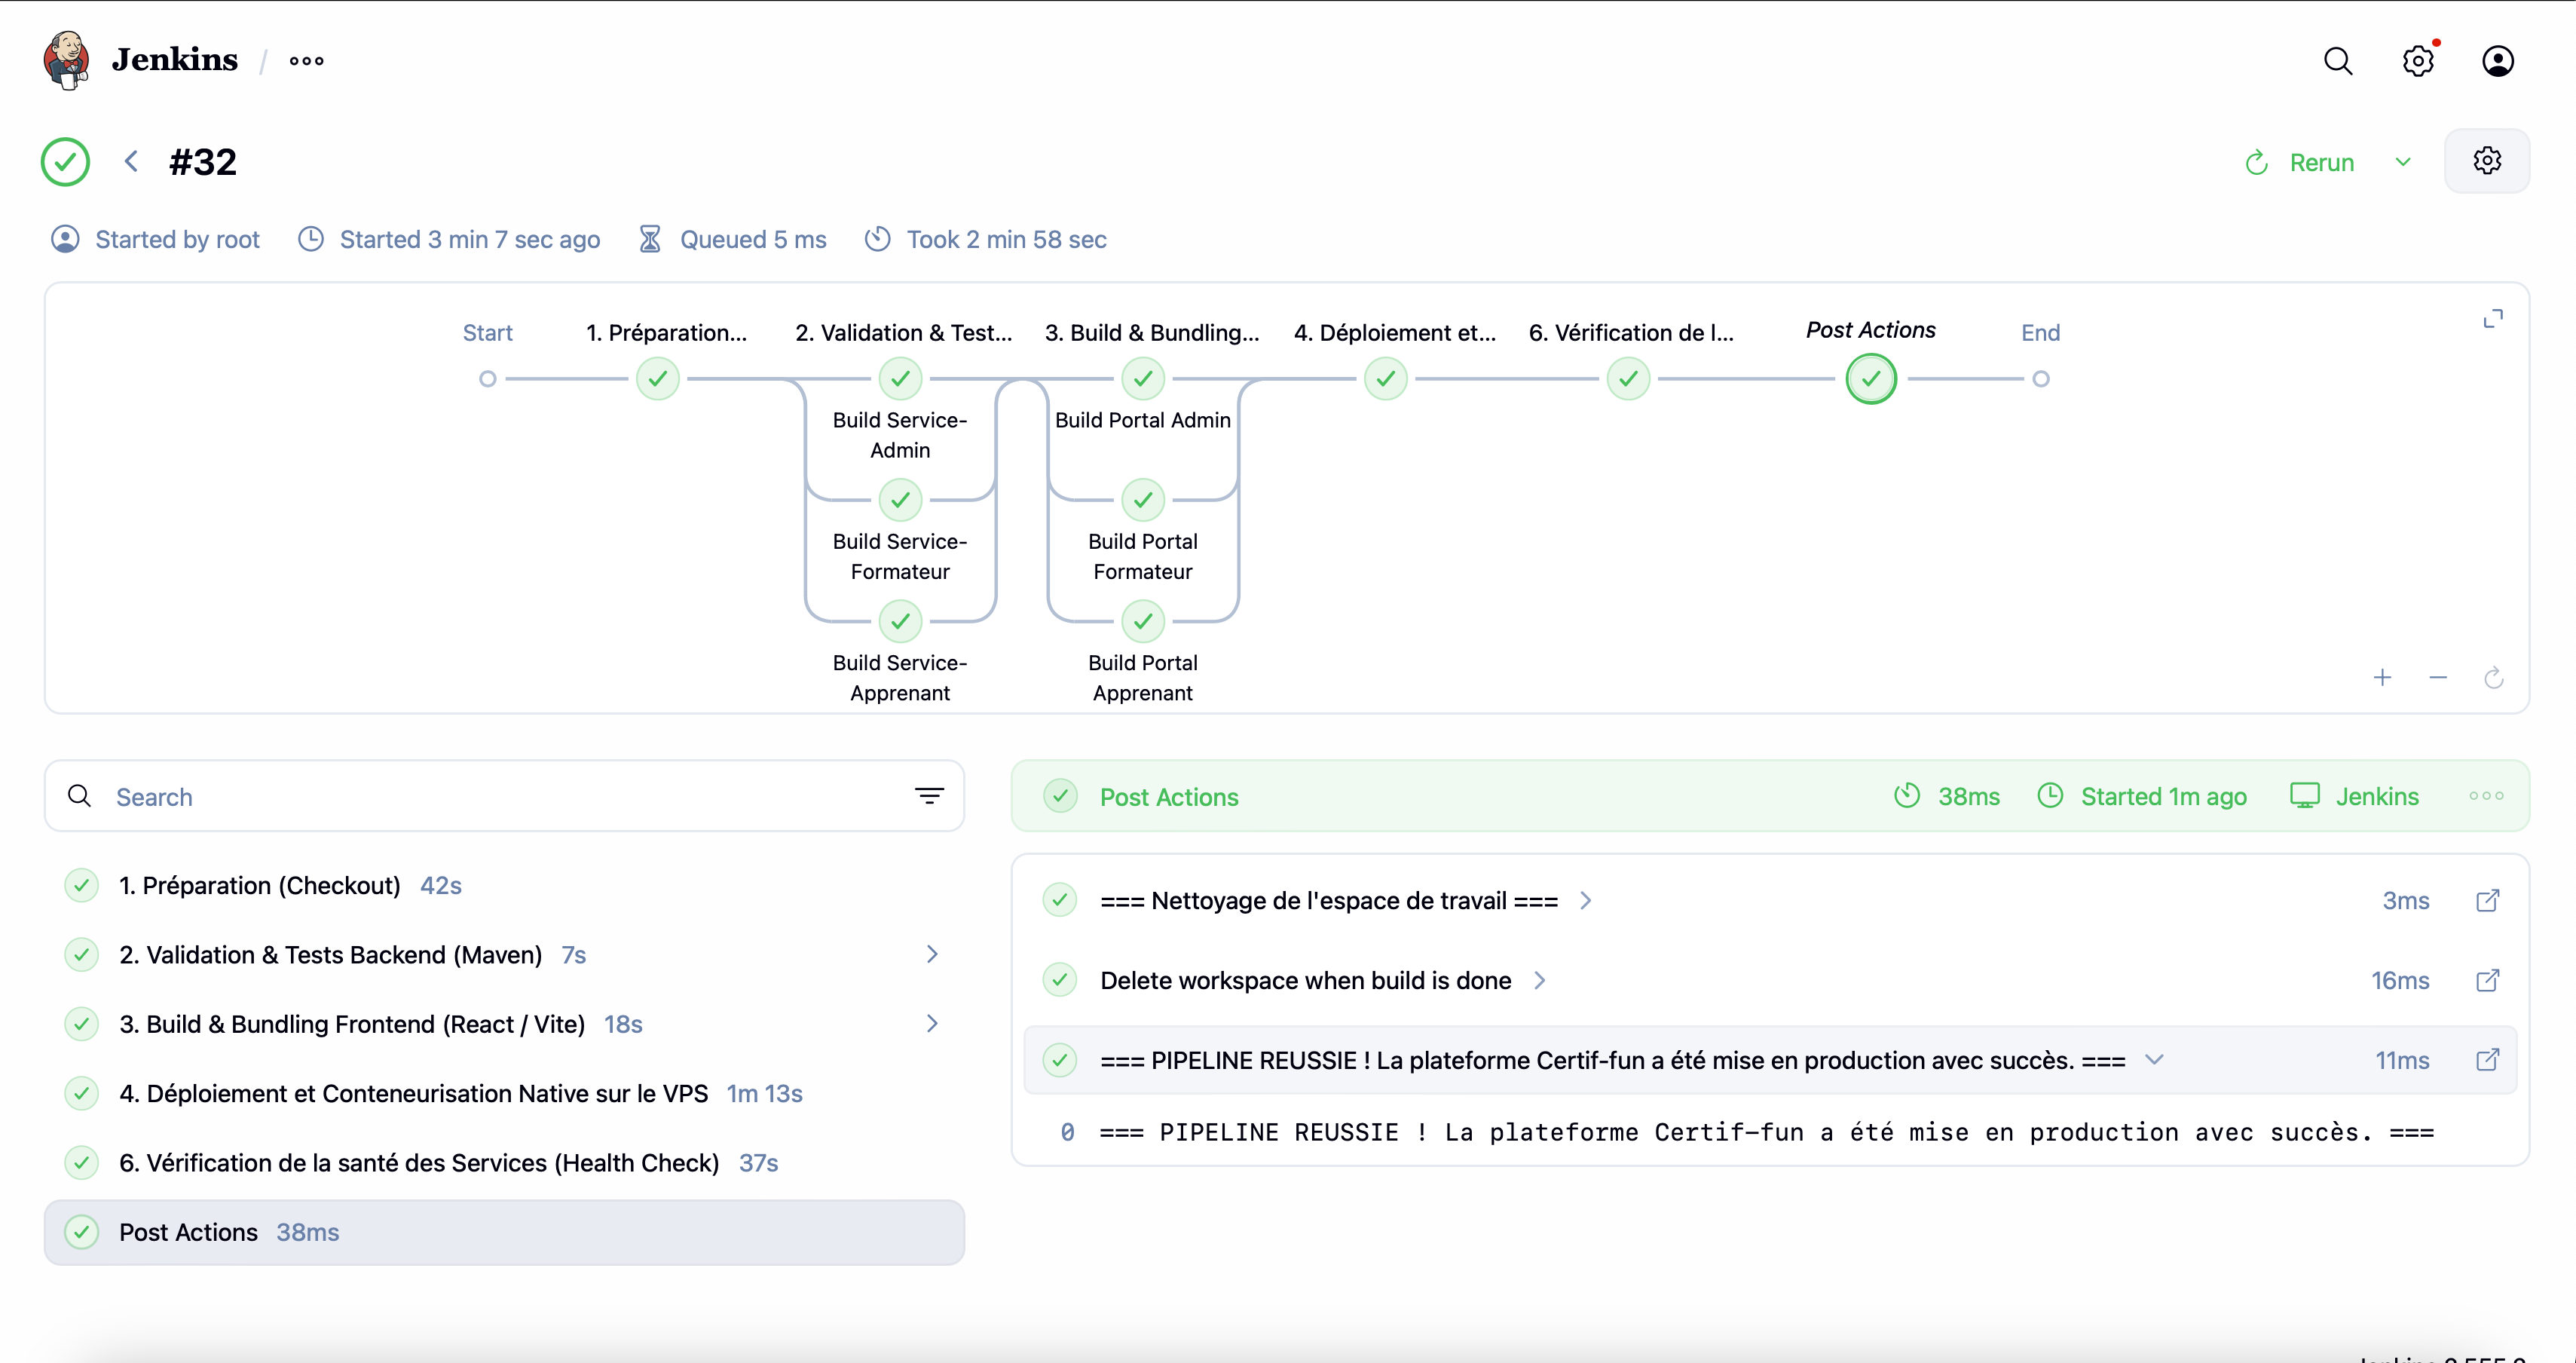
\includegraphics[width=0.98\textwidth]{figures/jenkins_pipeline.png}
    \caption{Interface de suivi visuel Jenkins présentant le succès de la build \#32 et le détail d'exécution séquentiel et parallèle des étapes du pipeline CI/CD.}
    \label{fig:jenkins_pipeline}
\end{figure}


\begin{enumerate}
    \item \textbf{Préparation [42s] :} Récupération sécurisée du code source via SSH et configuration automatique des environnements Node.js et Maven. Cette étape garantit un espace de build stable, portable et reproductible pour l'ensemble du projet. Elle permet de s'assurer que toutes les dépendances système sont prêtes avant le début de la compilation.

    \item \textbf{Compilation Backend [7s] :} Construction simultanée des trois microservices Spring Boot en parallèle pour optimiser les ressources. Cette méthode de compilation distribuée réduit drastiquement le temps de traitement global sur le serveur de build. Elle génère les artifacts exécutables nécessaires au déploiement des services métiers.

    \item \textbf{Compilation Frontend [18s] :} Génération et optimisation des trois interfaces React à l'aide du bundler Vite. Les fichiers statiques sont ainsi préparés et compressés pour une diffusion ultra-rapide sur le serveur web de production. Cette étape inclut la validation du typage TypeScript pour garantir la robustesse des interfaces.

    \item \textbf{Déploiement sur le VPS [1m 13s] :} Transfert de l'archive vers le serveur de production et mise à jour des conteneurs via Docker Compose. Une sauvegarde automatique de la base de données PostgreSQL est effectuée avant chaque mise à jour pour prévenir toute perte de données. Enfin, un nettoyage des images Docker orphelines libère l'espace disque du serveur.

    \item \textbf{Vérification de santé (Health Check) [37s] :} Contrôle automatique de la disponibilité des services via des requêtes sur les endpoints Actuator et la passerelle Nginx. Le pipeline s'interrompt immédiatement en cas d'anomalie détectée pour garantir la stabilité de la production. Cette étape valide que la nouvelle version est pleinement opérationnelle avant de clôturer la build.

    \item \textbf{Nettoyage local [< 1s] :} Purge complète de l'espace de travail sur l'agent Jenkins pour libérer les ressources disque après le succès du déploiement. Cette maintenance automatique évite l'encombrement du serveur de build sur le long terme. Elle assure que chaque nouveau pipeline démarre dans un environnement vierge et sain.
\end{enumerate}

Ce pipeline Jenkins assure des déploiements rapides, sécurisés et automatisés, garantissant l'intégrité et la disponibilité continue de la plateforme \textbf{Certif-fun}.


%%%%%%%%%%%%%%%%%%%%%%%%%%%%%%%%%%%%%%%%%%%%%%%%%%%%%%%%%%%
\section{Implémentation et interfaces}
%%%%%%%%%%%%%%%%%%%%%%%%%%%%%%%%%%%%%%%%%%%%%%%%%%%%%%%%%%%
L'implémentation de la plateforme \textbf{Certif-fun} est conçue selon un découpage strict des responsabilités en couches isolées, respectant le principe de séparation des préoccupations (\textit{Separation of Concerns}). Cette architecture se divise en trois couches principales : la présentation (Front-end), la logique métier (Back-end) et la persistance des données.

\subsection{Découpage architectural global}
Pour comprendre le fonctionnement global de la plateforme de manière simple, les requêtes transitent à travers les couches suivantes :
\begin{itemize}
    \item \textbf{Couche de Présentation (Front-end) :} Développée avec \textbf{React, TypeScript et Vite}. Elle fournit des interfaces fluides, interactives et responsives pour les trois types d'utilisateurs. Elle communique avec le serveur via des requêtes HTTP asynchrones gérées par la bibliothèque \textbf{Axios}.
    \item \textbf{Couche Logique Métier (Back-end) :} Composée de trois microservices indépendants développés avec \textbf{Spring Boot} (Java 17). Chaque microservice gère un domaine fonctionnel précis de la plateforme. En parallèle, un microservice Python développé avec \textbf{FastAPI} orchestre le modèle de détection visuelle \textbf{YOLOv8} pour la surveillance d'examen (Proctoring).
    \item \textbf{Couche de Données (Persistance) :} Repose sur le système de gestion de base de données relationnelle \textbf{PostgreSQL}. La couche de persistance Java utilise \textbf{Spring Data JPA} (Hibernate) pour manipuler les données sous forme d'objets (mapping objet-relationnel), évitant d'écrire des requêtes SQL manuelles complexes.
\end{itemize}

\subsection{Structure et organisation du code Backend (Spring Boot)}
Chacun des microservices Java (Admin, Formateur et Apprenant) est organisé selon une architecture en couches standardisée pour faciliter sa maintenance :
\begin{itemize}
    \item \textbf{\texttt{config} (Configuration) :} Regroupe les classes de paramétrage global de l'application (configurations CORS, initialisation des données par défaut via \texttt{DataInitializer}, et beans système).
    \item \textbf{\texttt{controller} (Contrôleurs REST) :} Représente le point d'entrée des requêtes HTTP. Il définit les URLs des APIs (points de terminaison comme \path{/api/v1/courses}), intercepte les requêtes envoyées par le frontend React, valide les données reçues et renvoie les réponses au format JSON.
    \item \textbf{\texttt{service} (Logique Métier) :} C'est le cœur applicatif. Ce package contient les classes implémentant les règles fonctionnelles (calculs de progression, traitement des examens, validation d'éligibilité aux certificats, cryptage de mots de passe, et dialogues avec le serveur de visioconférence LiveKit ou avec l'IA Ollama).
    \item \textbf{\texttt{repository} (Accès aux Données) :} Contient les interfaces de persistance héritant de \texttt{JpaRepository}. Elles permettent d'exécuter des opérations de lecture et d'écriture (CRUD) dans la base de données PostgreSQL de manière abstraite.
    \item \textbf{\texttt{model} (Entités) :} Définit les classes Java annotées avec \texttt{@Entity} représentant la structure de nos tables PostgreSQL (ex. \texttt{Course}, \texttt{Quiz}, \texttt{Apprenant}, \texttt{EncadrementPhase}).
    \item \textbf{\texttt{dto} (Data Transfer Objects) :} Classes simples utilisées pour structurer les données transférées entre le frontend et le backend (ex. \texttt{AuthenticationRequest}, \texttt{QuizStatisticsDTO}), permettant de ne pas exposer directement les entités de la base de données.
    \item \textbf{\texttt{security} (Sécurité JWT) :} Contient le filtre \texttt{JwtAuthenticationFilter} qui extrait et valide le jeton de connexion des requêtes entrantes pour authentifier l'utilisateur.
\end{itemize}

\subsection{Structure et organisation du code Frontend (React)}
Les trois applications frontales (\texttt{Service Admin}, \texttt{Service Formateur} et \texttt{Service Apprenant}) adoptent une structure modulaire, claire et réutilisable :
\begin{itemize}
    \item \textbf{\texttt{pages/} (Vues Principales) :} Contient les composants représentant les pages entières de l'application (ex. \path{Dashboard.tsx}, \path{Examen.tsx}, \path{Parametres.tsx}).
    \item \textbf{\texttt{components/} (Éléments UI Réutilisables) :} Regroupe les blocs visuels génériques et autonomes réutilisés sur plusieurs pages (boutons stylisés, barres de progression, modales d'alertes, cartes d'affichage de cours).
    \item \textbf{\texttt{api/} (Connexion API) :} Regroupe les configurations d'Axios, les intercepteurs pour ajouter automatiquement le token JWT dans les en-têtes HTTP de chaque requête, et les fonctions d'appel aux microservices backend.
    \item \textbf{\texttt{context/} (Gestion d'État Global) :} Contient les contextes React (ex. \texttt{AuthContext}) permettant de partager des informations globales (comme l'état de connexion de l'utilisateur ou ses droits d'accès) à l'ensemble des pages.
    \item \textbf{\texttt{hooks/} (Hooks Personnalisés) : } Fichiers encapsulant de la logique réutilisable (gestion du flux de la caméra web pour le proctoring, sélection de périphériques média).
    \item \textbf{\texttt{types/} (Typages TypeScript) :} Contient les interfaces TypeScript décrivant la forme des données reçues des API pour sécuriser l'écriture du code (auto-complétion, détection précoce d'erreurs de typage).
\end{itemize}

\subsection{Structure du service de traitement d'images (IA Proctoring)}
Le dossier \path{AI-Detection-Service} est structuré de façon minimale pour optimiser la rapidité d'exécution du traitement vidéo :
\begin{itemize}
    \item \textbf{\texttt{main.py} (Script principal) :} Initialise le serveur FastAPI, charge le modèle pré-entraîné YOLOv8 en mémoire (\texttt{yolov8n.pt}), et expose un point d'accès POST sécurisé. Il reçoit le flux d'images envoyé par le navigateur de l'apprenant sous format d'archive base64, décompresse l'image, applique les filtres de détection d'objets, et renvoie un dictionnaire JSON détaillant les anomalies identifiées (ex. détection de téléphone, nombre de visages).
    \item \textbf{\texttt{requirements.txt} (Dépendances Python) :} Liste les bibliothèques minimales nécessaires à l'exécution du service de vision par ordinateur (\texttt{fastapi}, \texttt{uvicorn}, \texttt{opencv-python-headless}, \texttt{ultralytics}).
\end{itemize}



\subsection{Interfaces utilisateur et scénarios de navigation}
L'ergonomie des interfaces de \textbf{Certif-fun} a été conçue pour offrir une expérience utilisateur (UX) fluide, immersive et moderne, articulée autour de trois portails distincts adaptés à chaque profil d'utilisateur. Dans cette section, nous présentons en détail les fonctionnalités offertes par chaque espace à travers des captures d'écran de l'application finale.

\subsubsection{Authentification et Accès}
Avant d'accéder aux différents portails, chaque utilisateur doit s'identifier.

La figure~\ref{fig:login} illustre la page de connexion sécurisée de la plateforme. Cette interface permet à l'utilisateur de s'authentifier en saisissant son adresse email et son mot de passe. Le système vérifie les identifiants et redirige l'utilisateur vers son espace dédié (Admin, Formateur ou Apprenant) en générant un jeton de session JWT.
\begin{figure}[H]
    \centering
    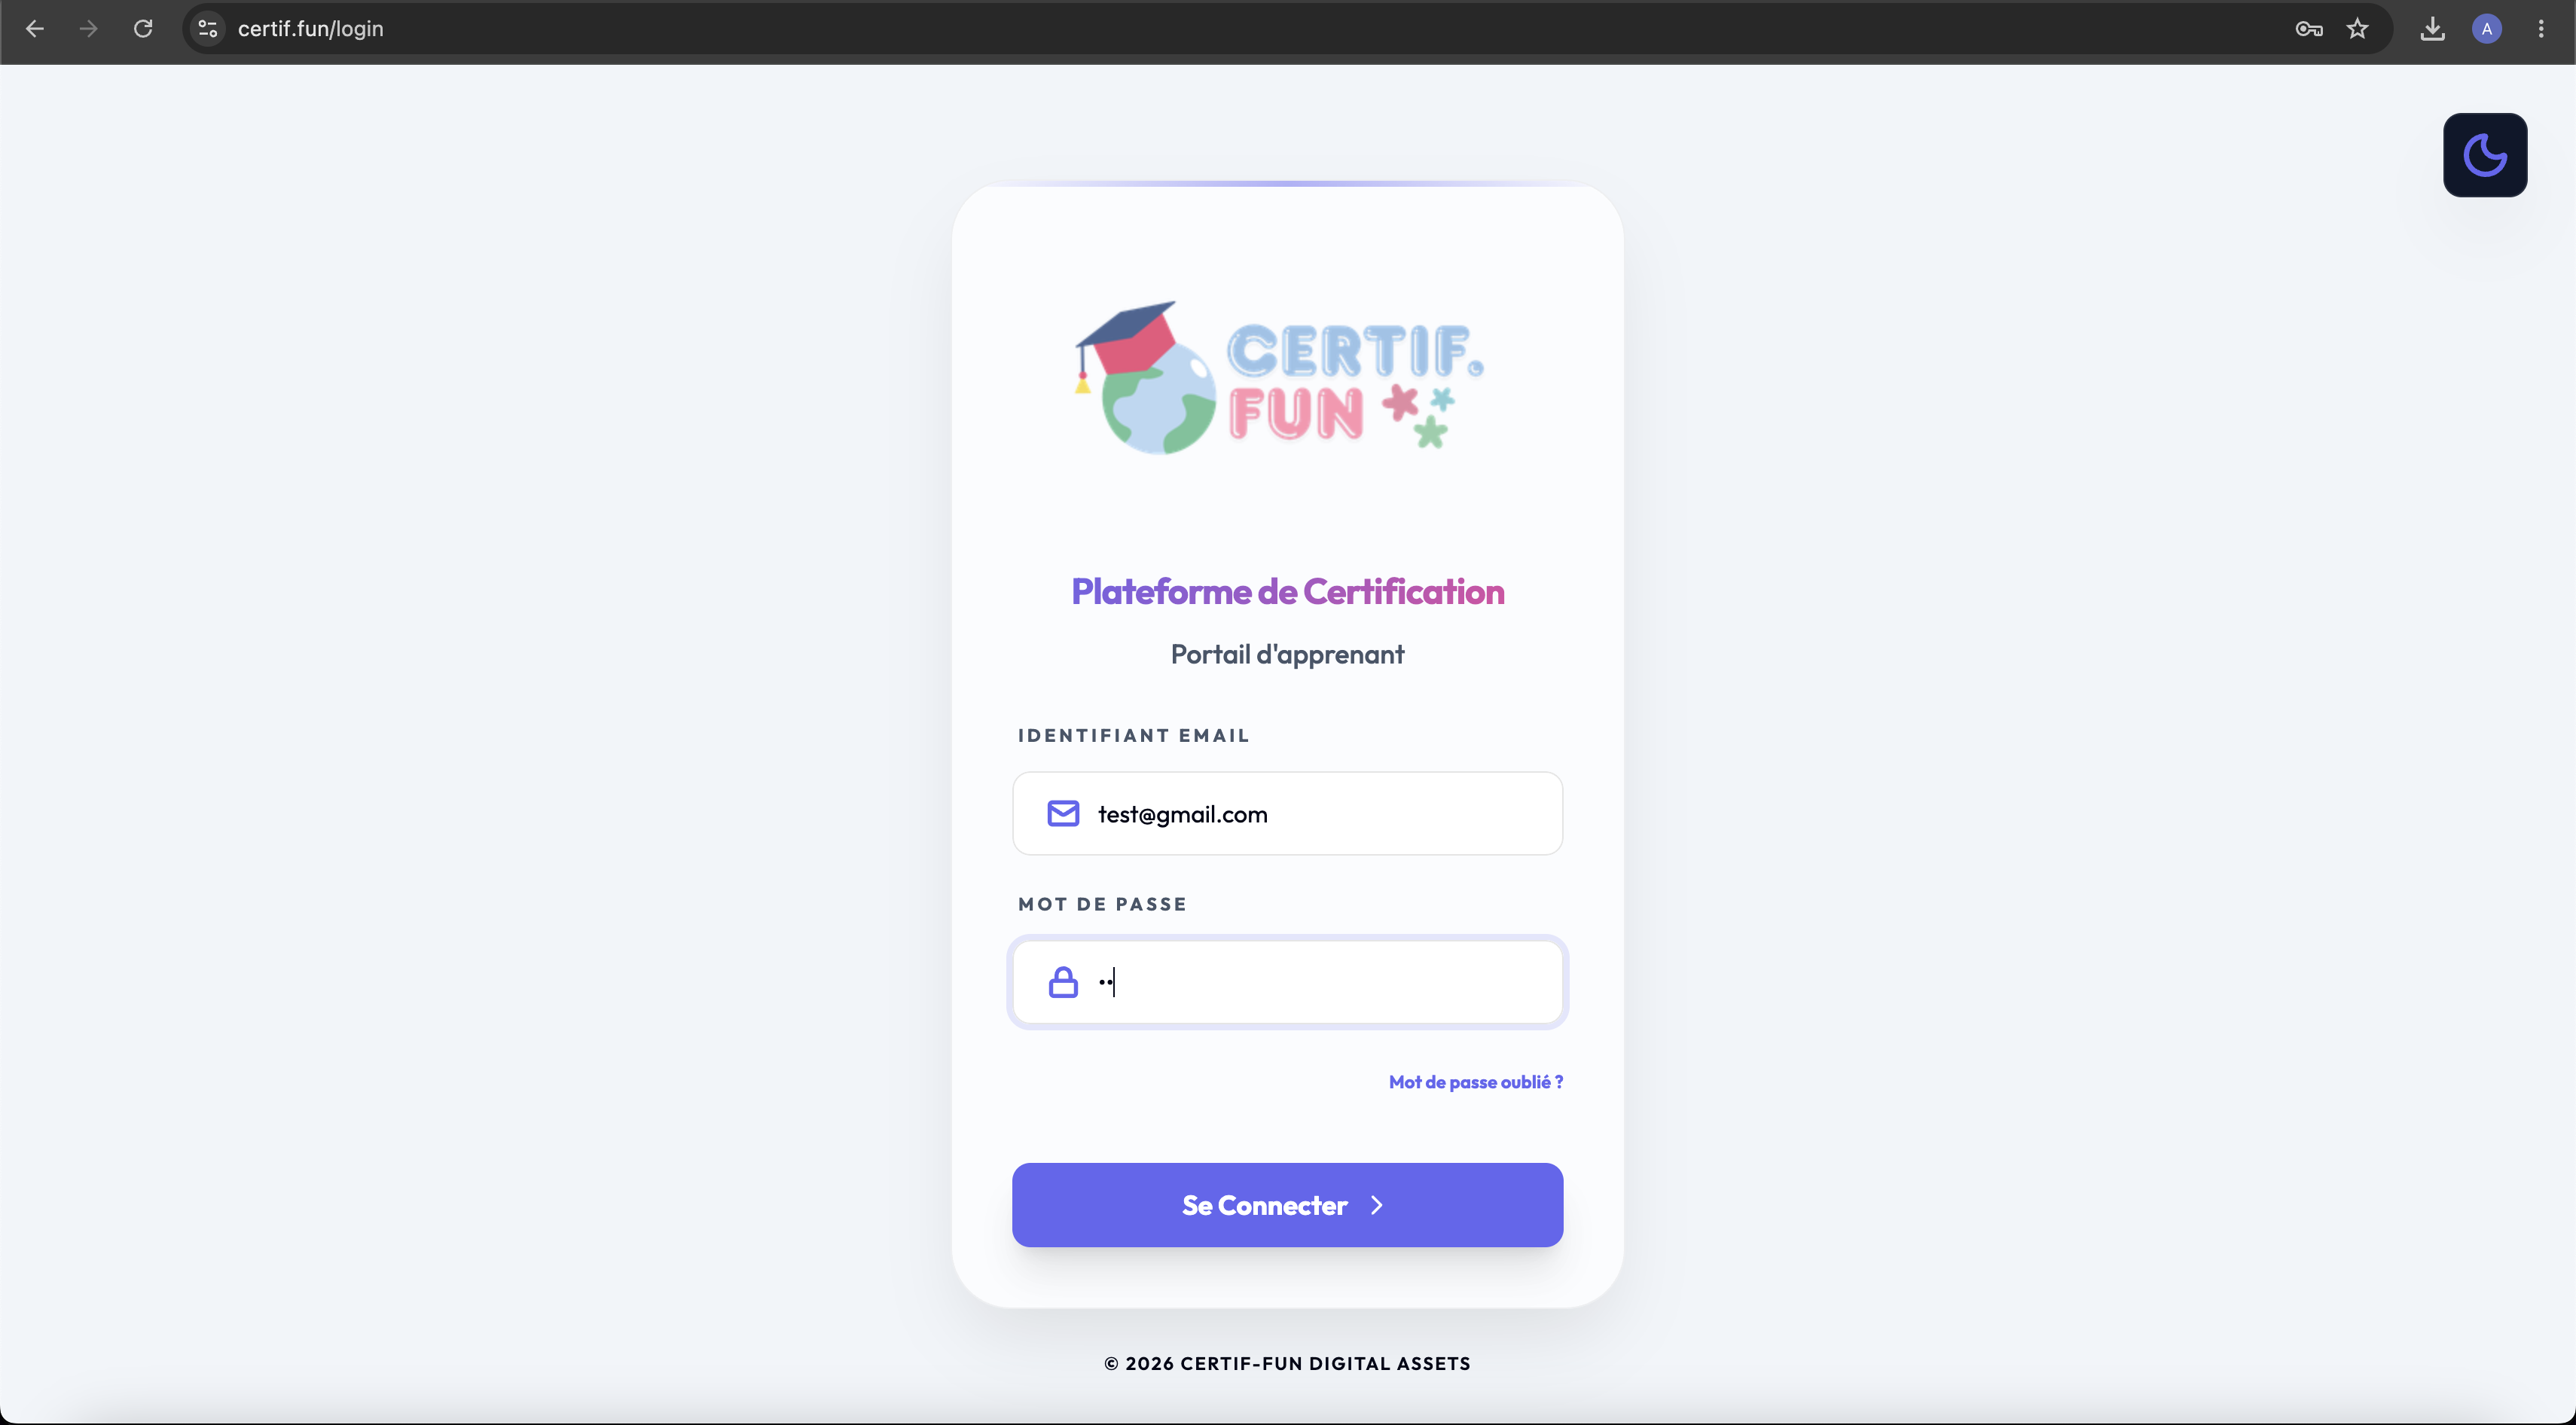
\includegraphics[width=0.98\textwidth]{figures/login.png}
    \caption{Interface de connexion à la plateforme}
    \label{fig:login}
\end{figure}

\subsubsection{Portail Administrateur}
L'espace d'administration centralise les outils de supervision et de configuration de la plateforme.

La figure~\ref{fig:admin1} présente le tableau de bord principal de l'administrateur. Cette interface offre une vue d'ensemble instantanée sur l'activité de la plateforme à travers plusieurs indicateurs clés de performance :
\begin{itemize}
    \item \textbf{Total Apprenants :} Affiche le nombre total d'étudiants inscrits sur la plateforme.
    \item \textbf{Total Formateurs :} Indique le nombre de professeurs et encadrants actifs.
    \item \textbf{Taux de Réussite :} Présente le pourcentage moyen de réussite aux évaluations sur l'ensemble des cours.
    \item \textbf{Nombre Certificats :} Indique le nombre de certifications délivrées aux apprenants.
\end{itemize}
Un graphique interactif permet également de retracer l'évolution mensuelle des inscriptions.
\begin{figure}[H]
    \centering
    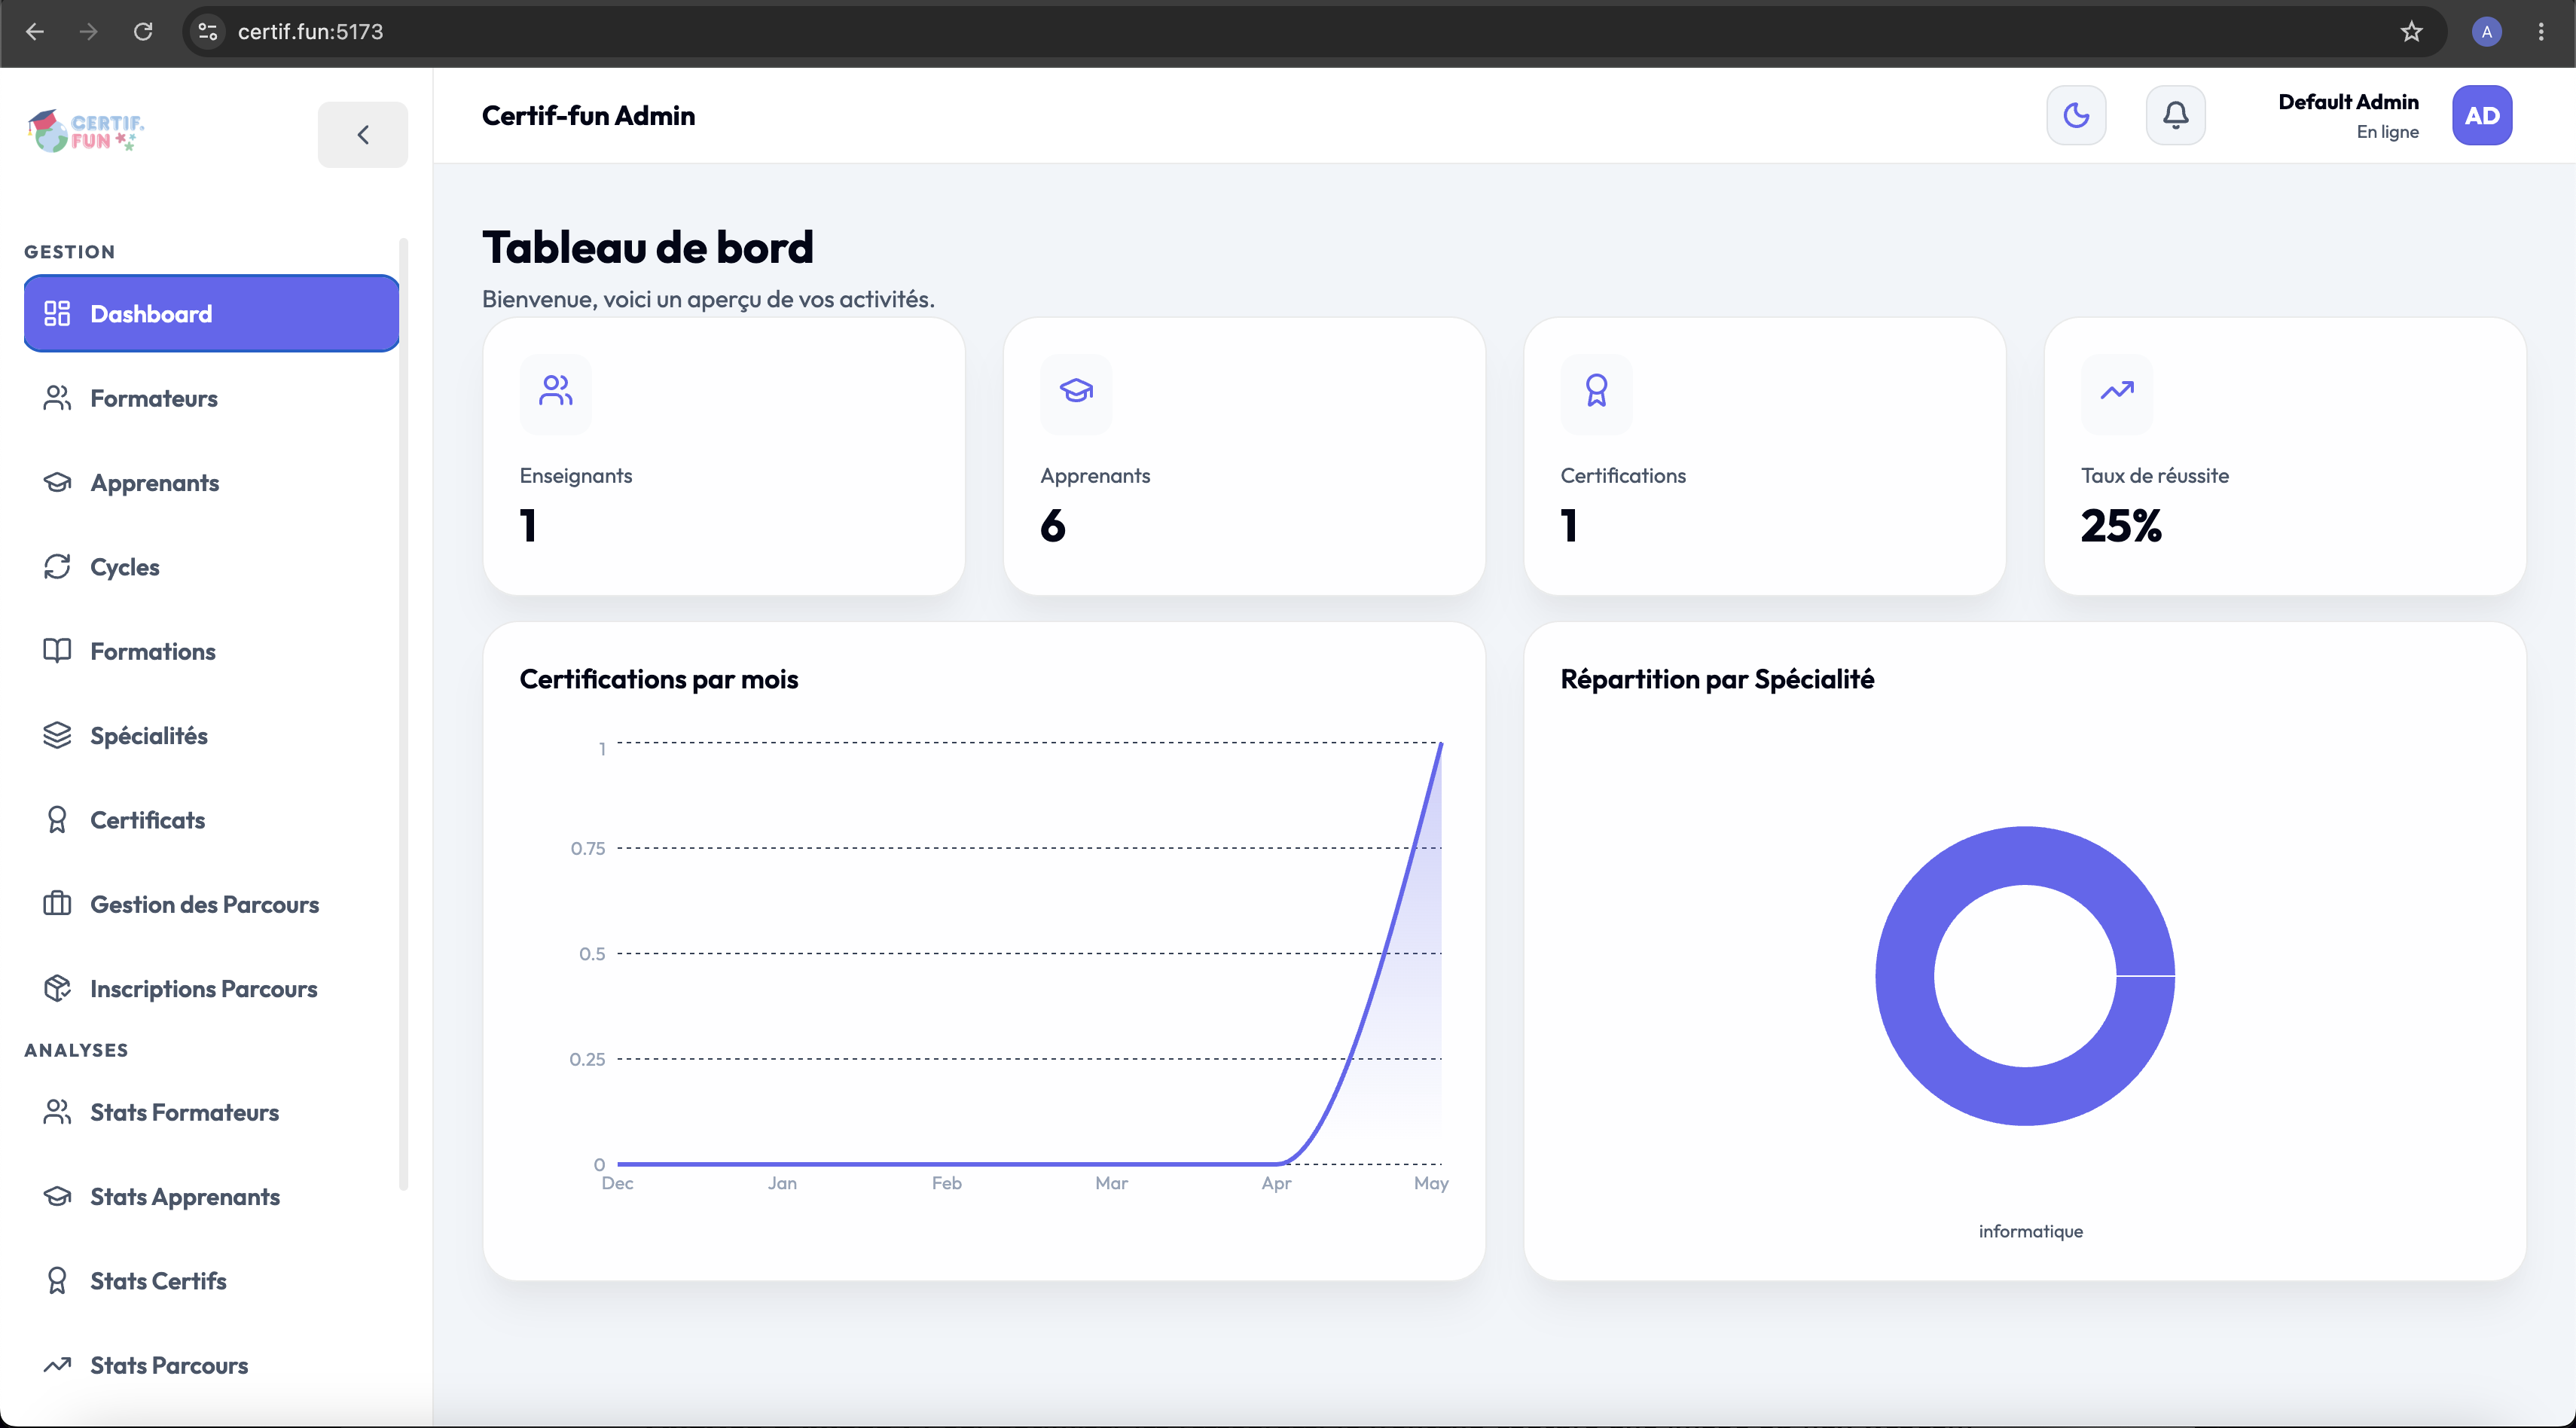
\includegraphics[width=0.98\textwidth]{figures/admin-1.png}
    \caption{Tableau de bord de l'Administrateur présentant les statistiques globales}
    \label{fig:admin1}
\end{figure}

La figure~\ref{fig:admin2} illustre le module de gestion des étudiants. L'administrateur dispose d'une liste complète des apprenants avec des outils de recherche rapide et de filtrage (par spécialité et statut). Il peut ajouter de nouveaux utilisateurs, modifier leurs informations ou restreindre leur accès si nécessaire. De plus, si l'apprenant est inséré correctement, il reçoit automatiquement un email pour s'authentifier à la plateforme.
\begin{figure}[H]
    \centering
    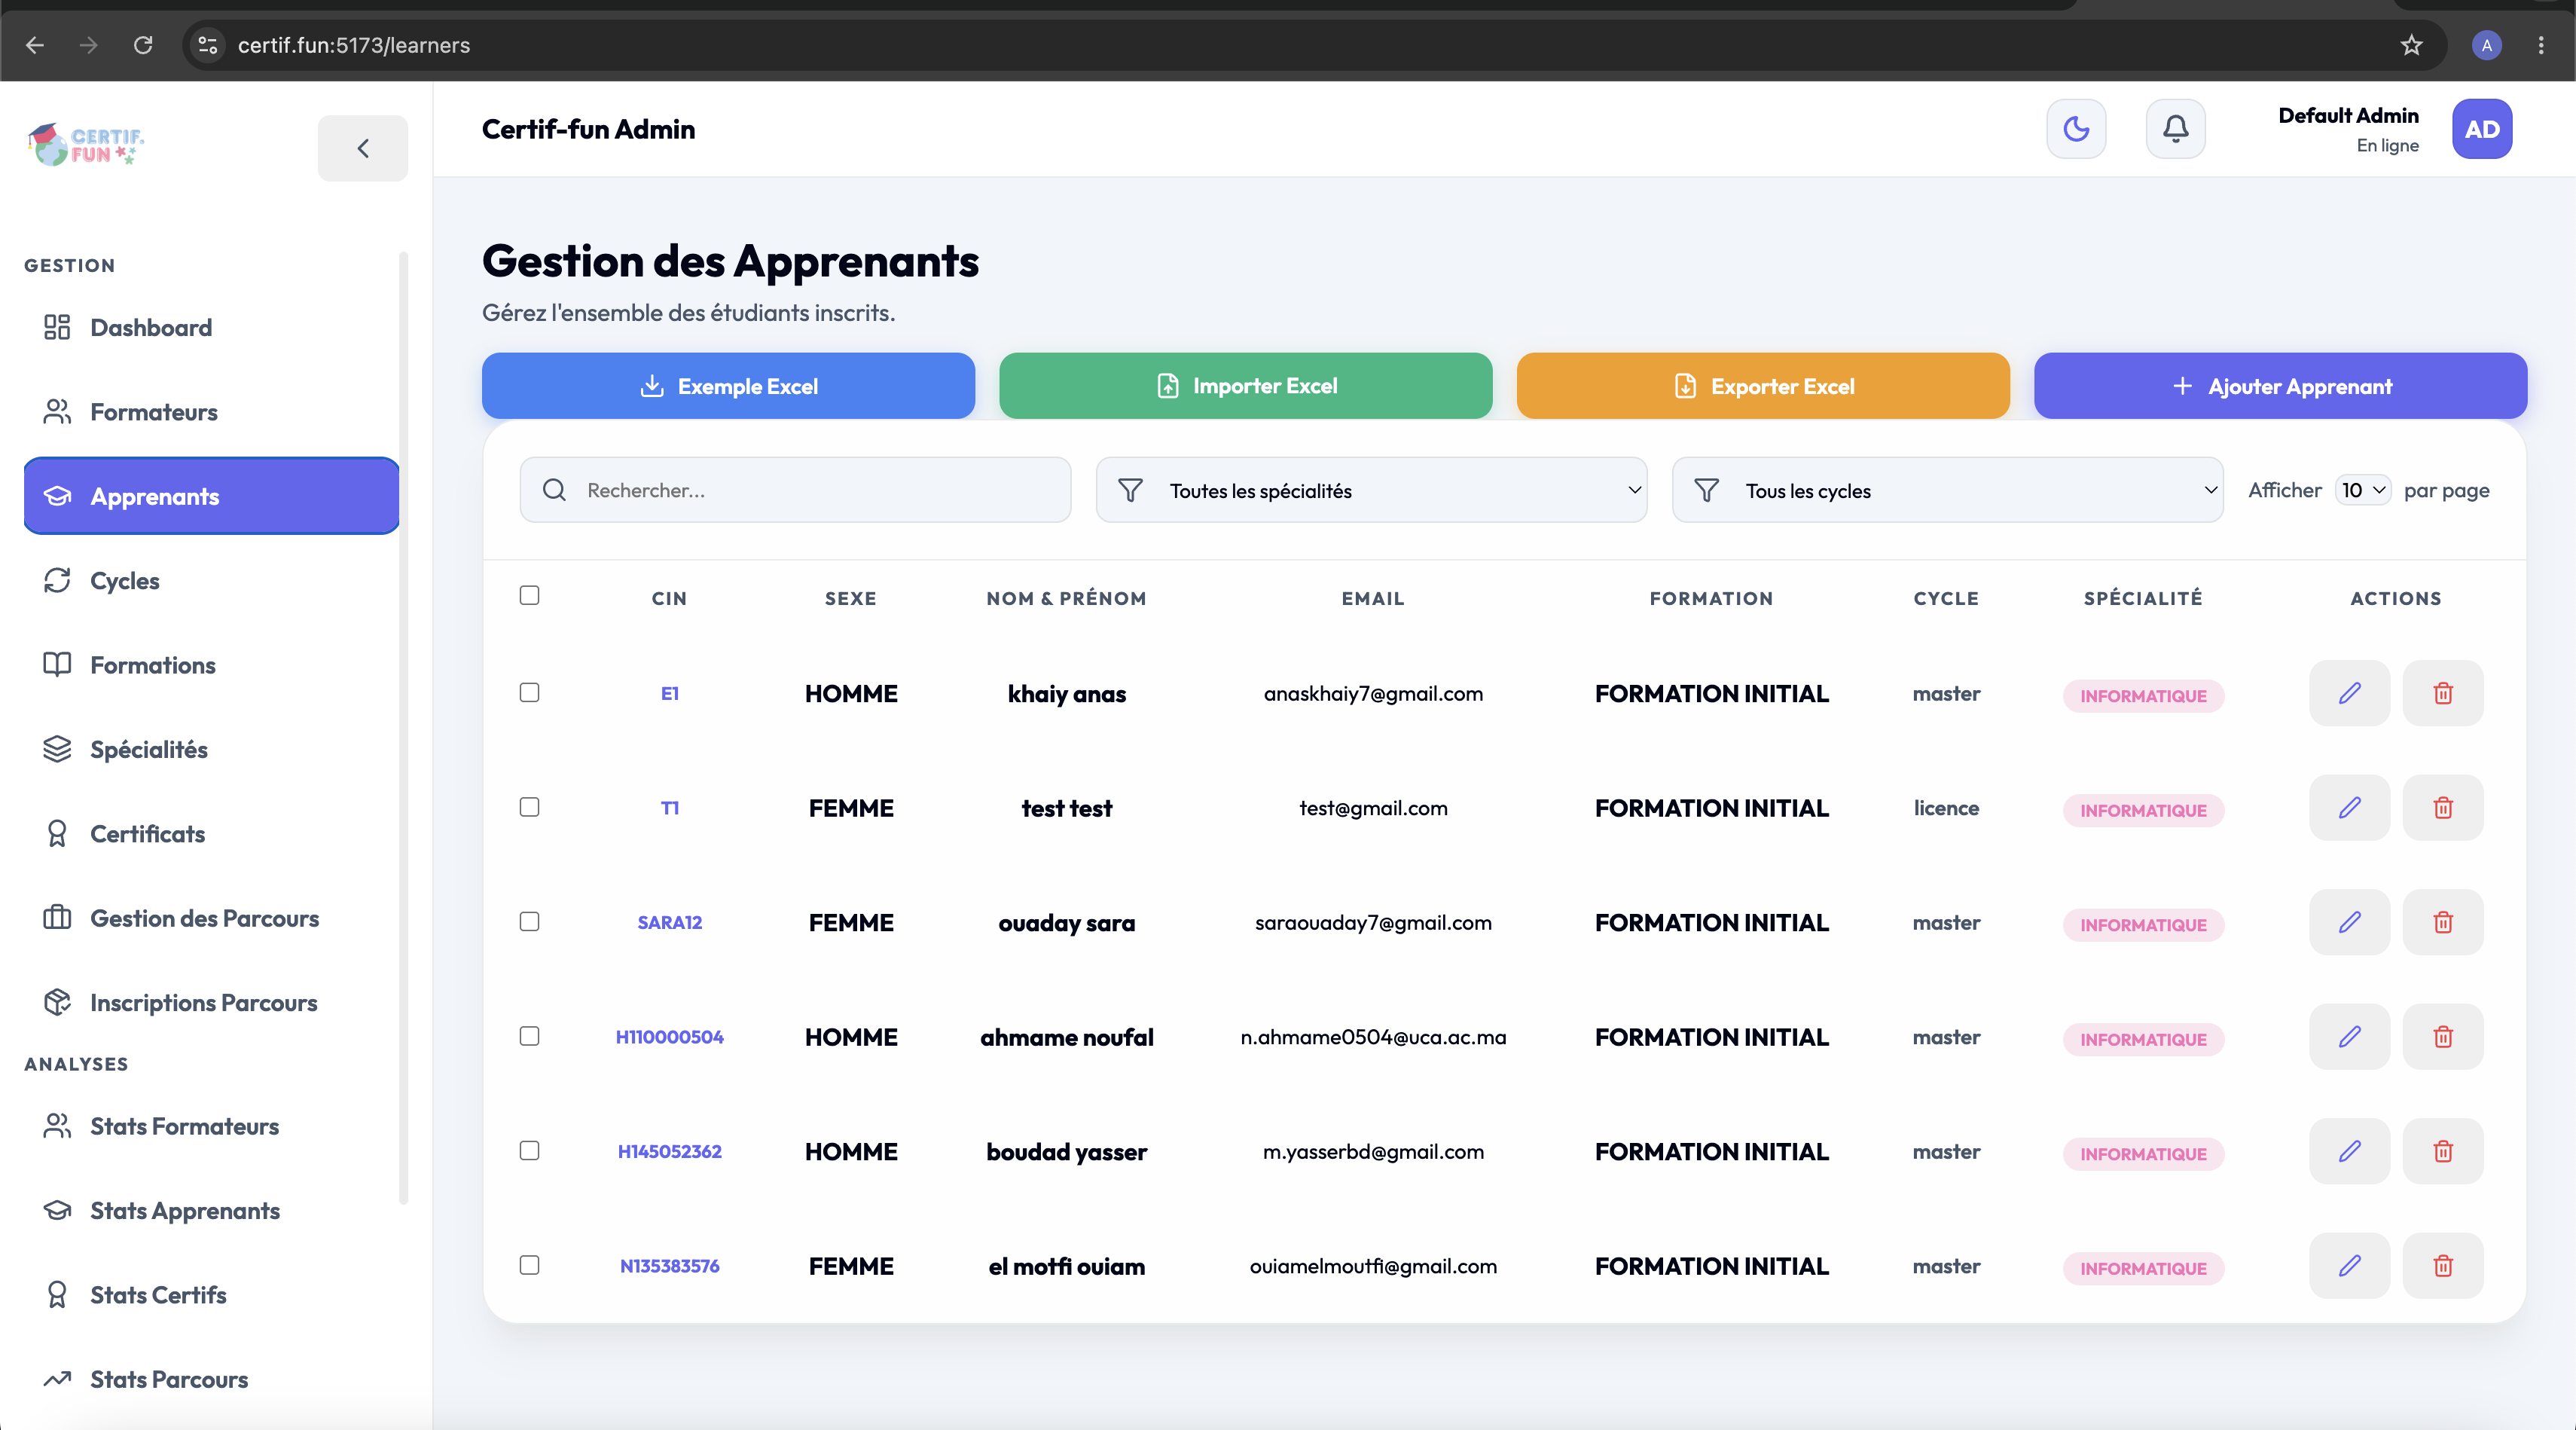
\includegraphics[width=0.98\textwidth]{figures/admin-2.png}
    \caption{Interface de gestion des étudiants}
    \label{fig:admin2}
\end{figure}

La section dédiée aux certificats (Figure~\ref{fig:admin3}) permet à l'administrateur d'ajuster le design des certificats, incluant le logo, la taille, le cachet et d'autres éléments visuels du certificat.
\begin{figure}[H]
    \centering
    
\includegraphics[width=0.98\textwidth]{figures/admin-3.png}
    \caption{Registre des certificats délivrés}
    \label{fig:admin3}
\end{figure}

La section dédiée aux parcours (Figure~\ref{fig:admin4}) permet aux formateurs de suivre un parcours qui contient plusieurs cours.
\begin{figure}[H]
    \centering
    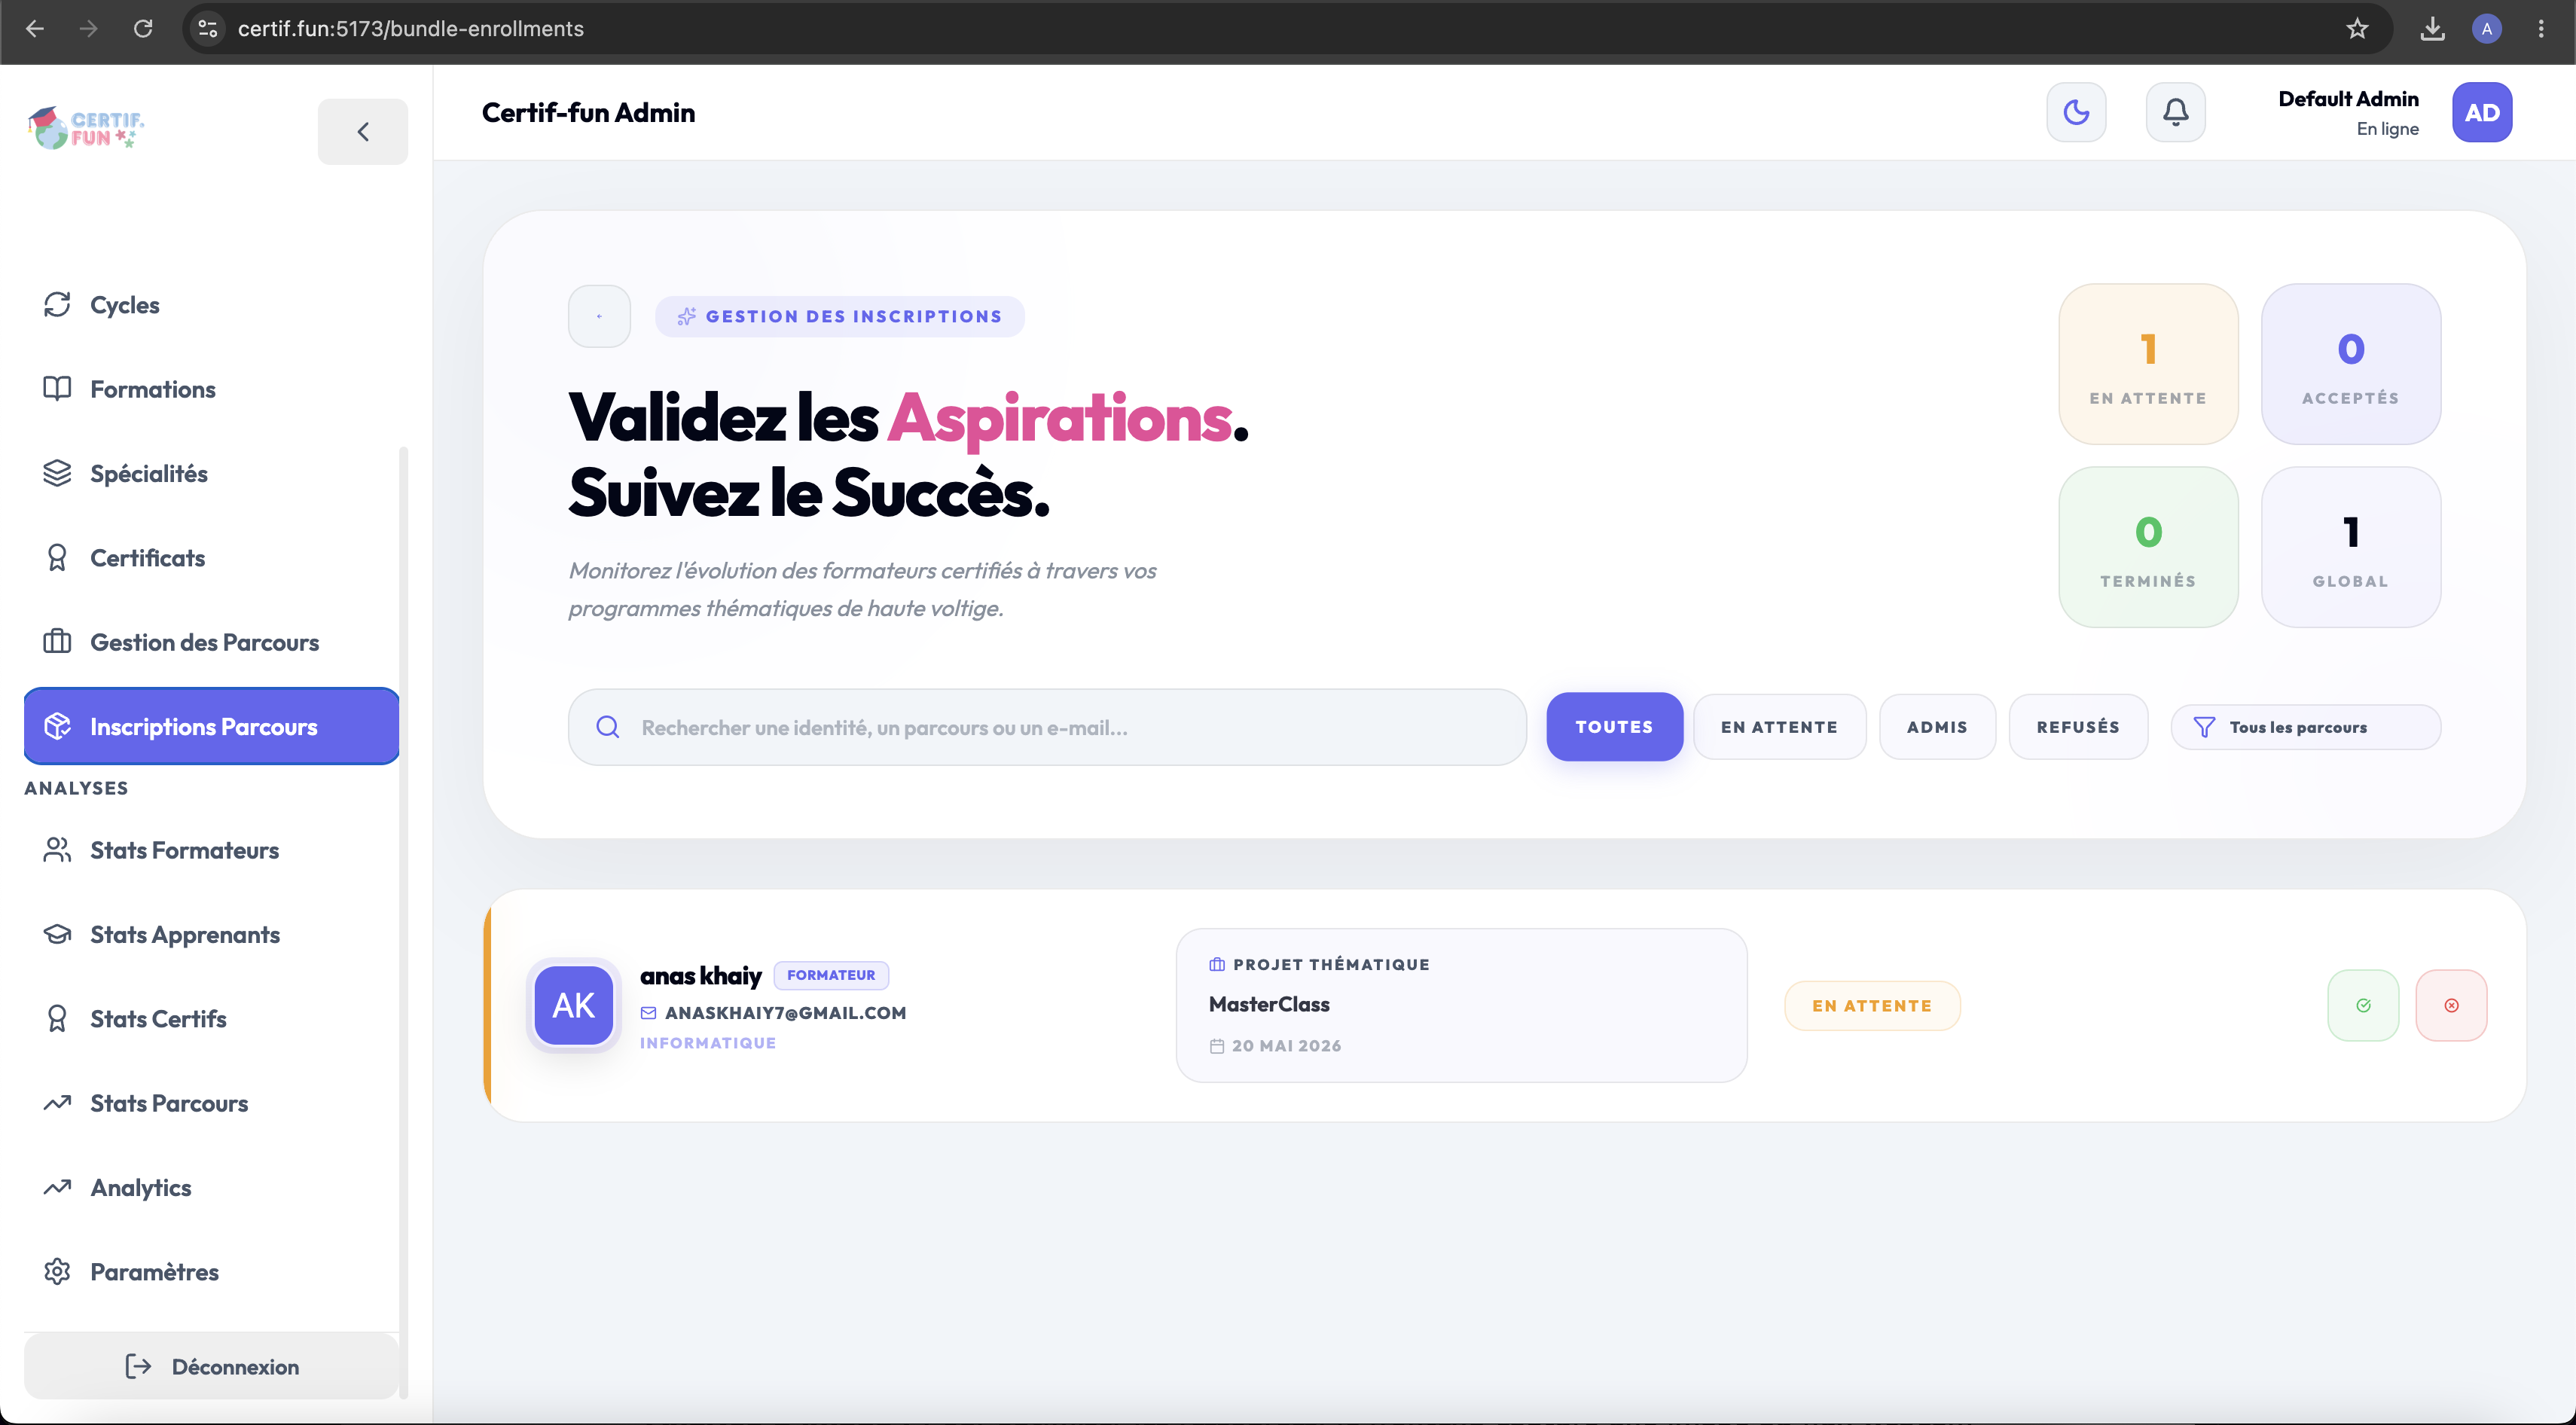
\includegraphics[width=0.98\textwidth]{figures/admin-4.png}
    \caption{Gestion des demandes d'inscription}
    \label{fig:admin4}
\end{figure}

\subsubsection{Portail Formateur}
L'espace Formateur est conçu pour faciliter la création de contenu pédagogique et le suivi des apprenants.

Le tableau de bord (Figure~\ref{fig:formateur1}) offre au formateur un résumé de son activité. Il y retrouve des statistiques sur ses apprenants, le taux de réussite global et le nombre de certificats délivrés aux étudiants.
\begin{figure}[H]
    \centering
    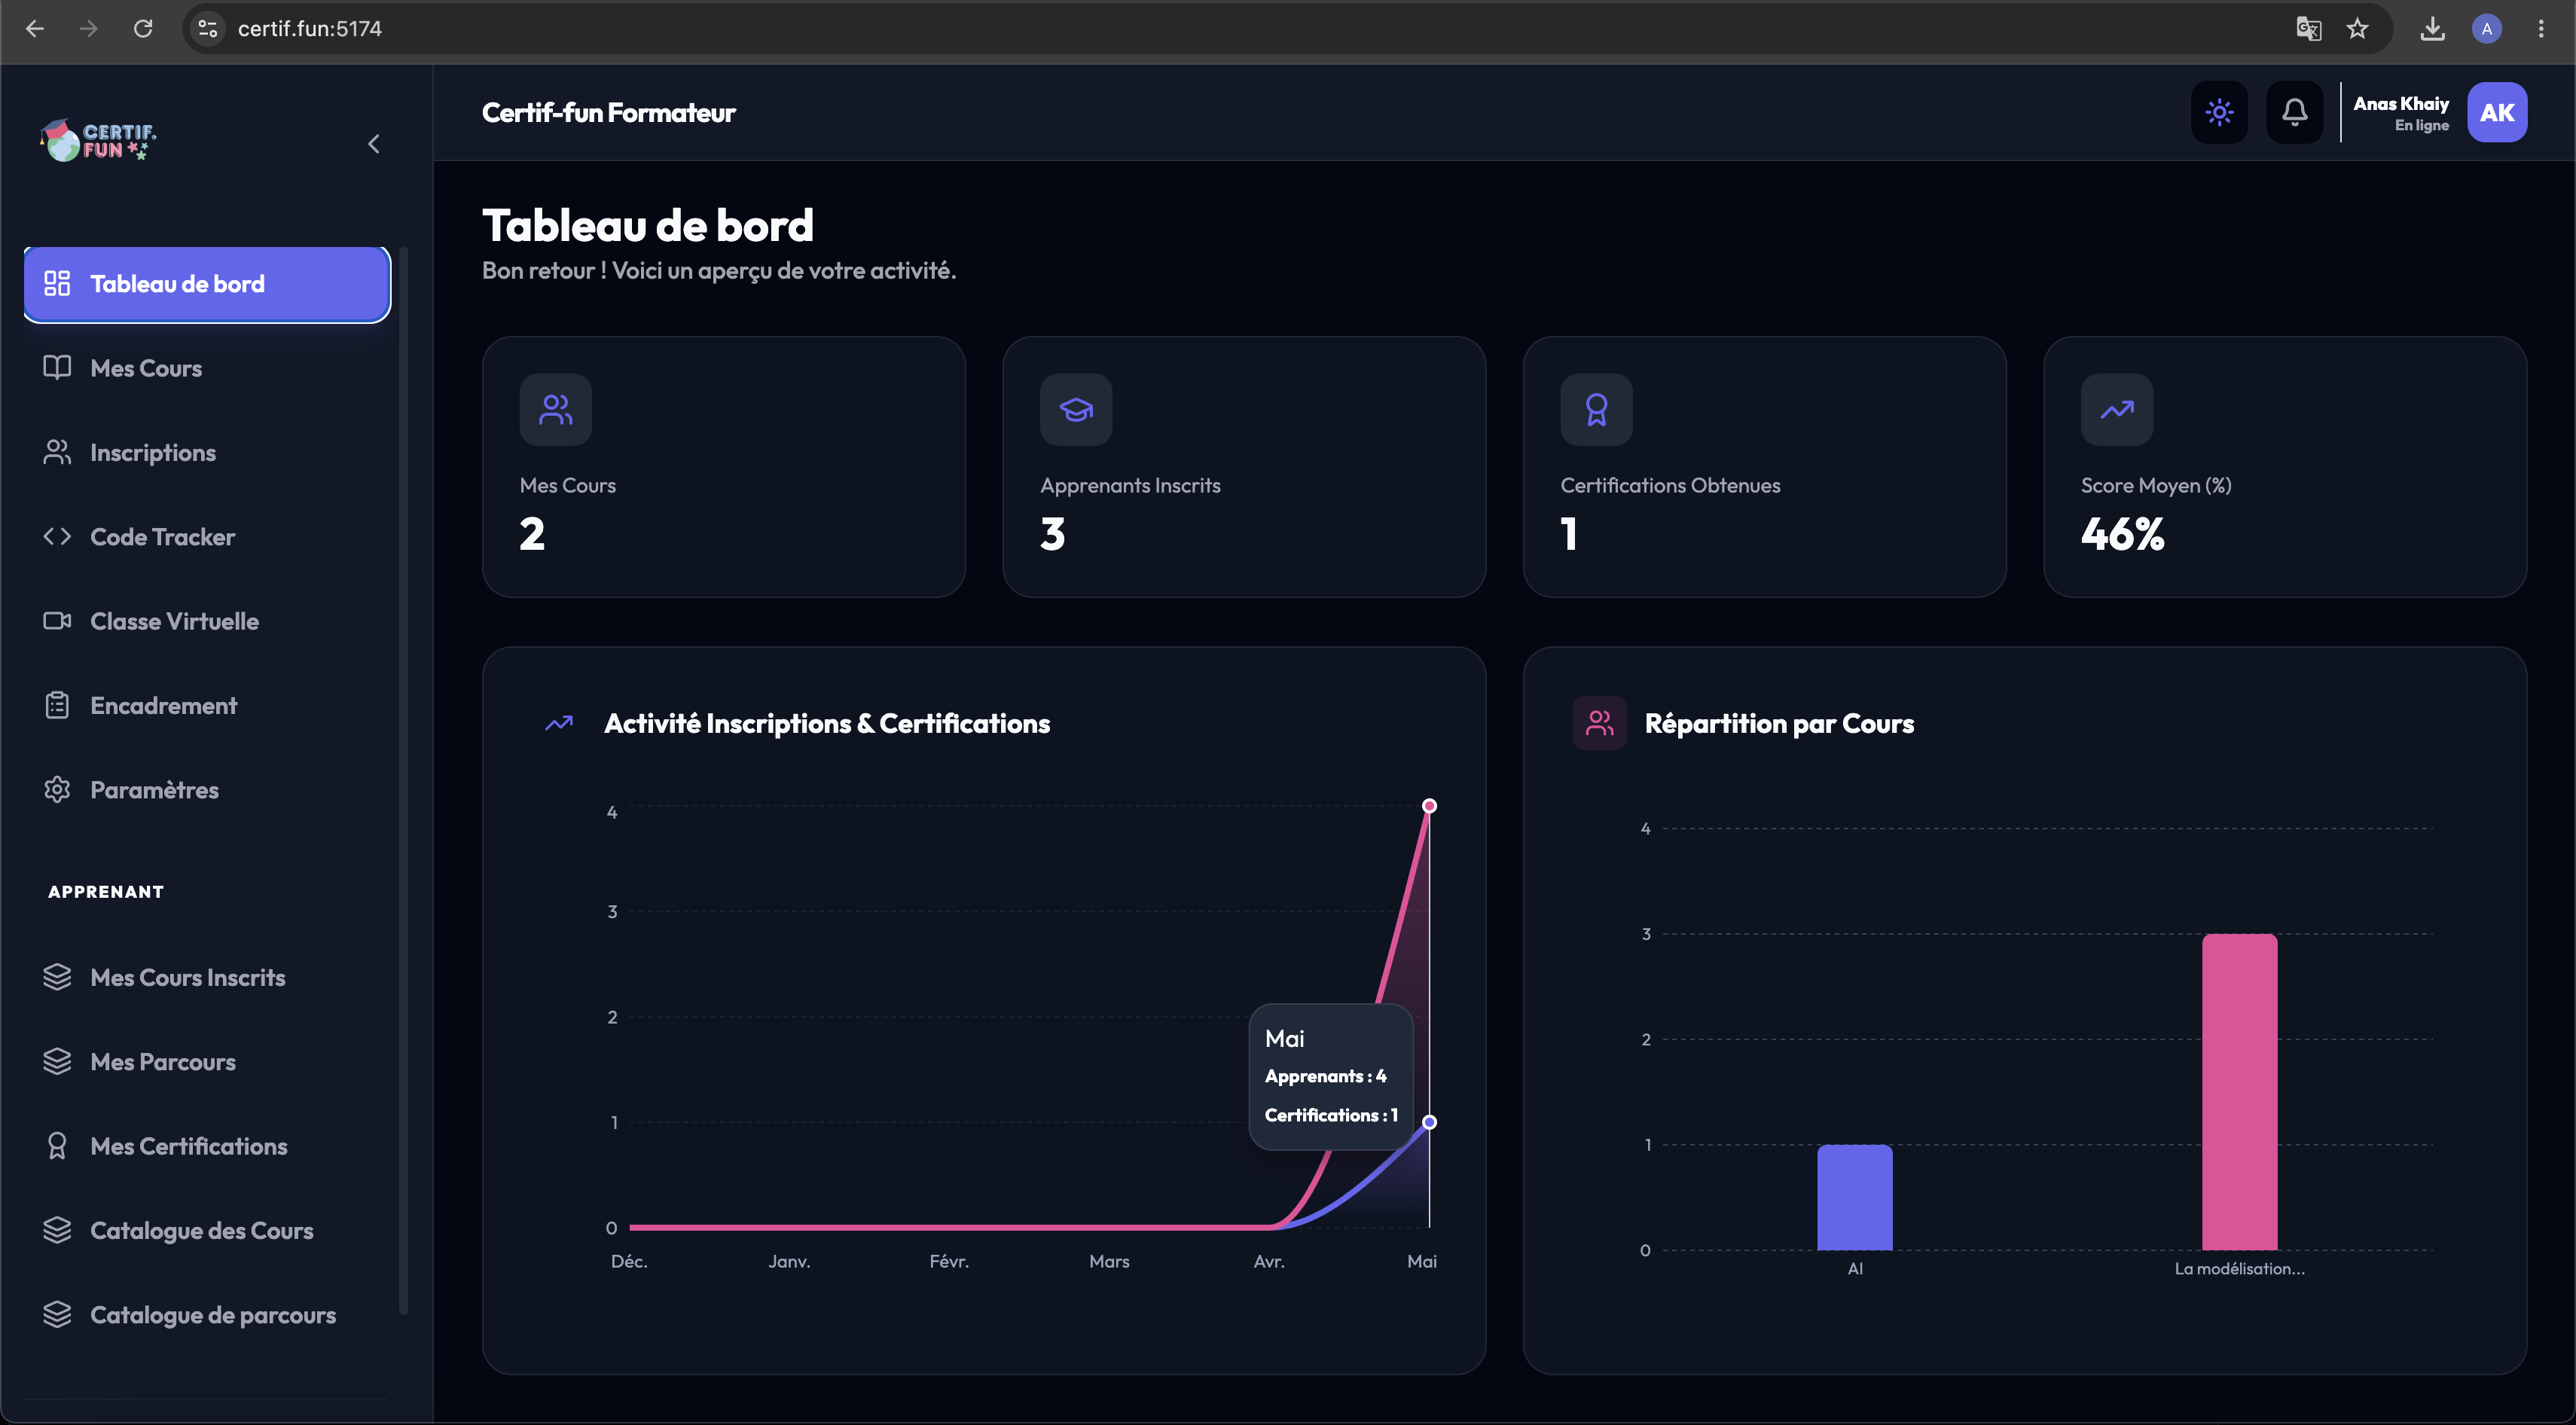
\includegraphics[width=0.98\textwidth]{figures/formateur-1.png}
    \caption{Tableau de bord du Formateur}
    \label{fig:formateur1}
\end{figure}

La vue "Mes Cours" (Figure~\ref{fig:formateur2}) permet au professeur de créer un cours avec plusieurs fonctionnalités avancées, telles que la définition d'une date limite pour finaliser la certification et un compteur pour afficher le nombre de minutes passées par l'apprenant dans la certification.
\begin{figure}[H]
    \centering
    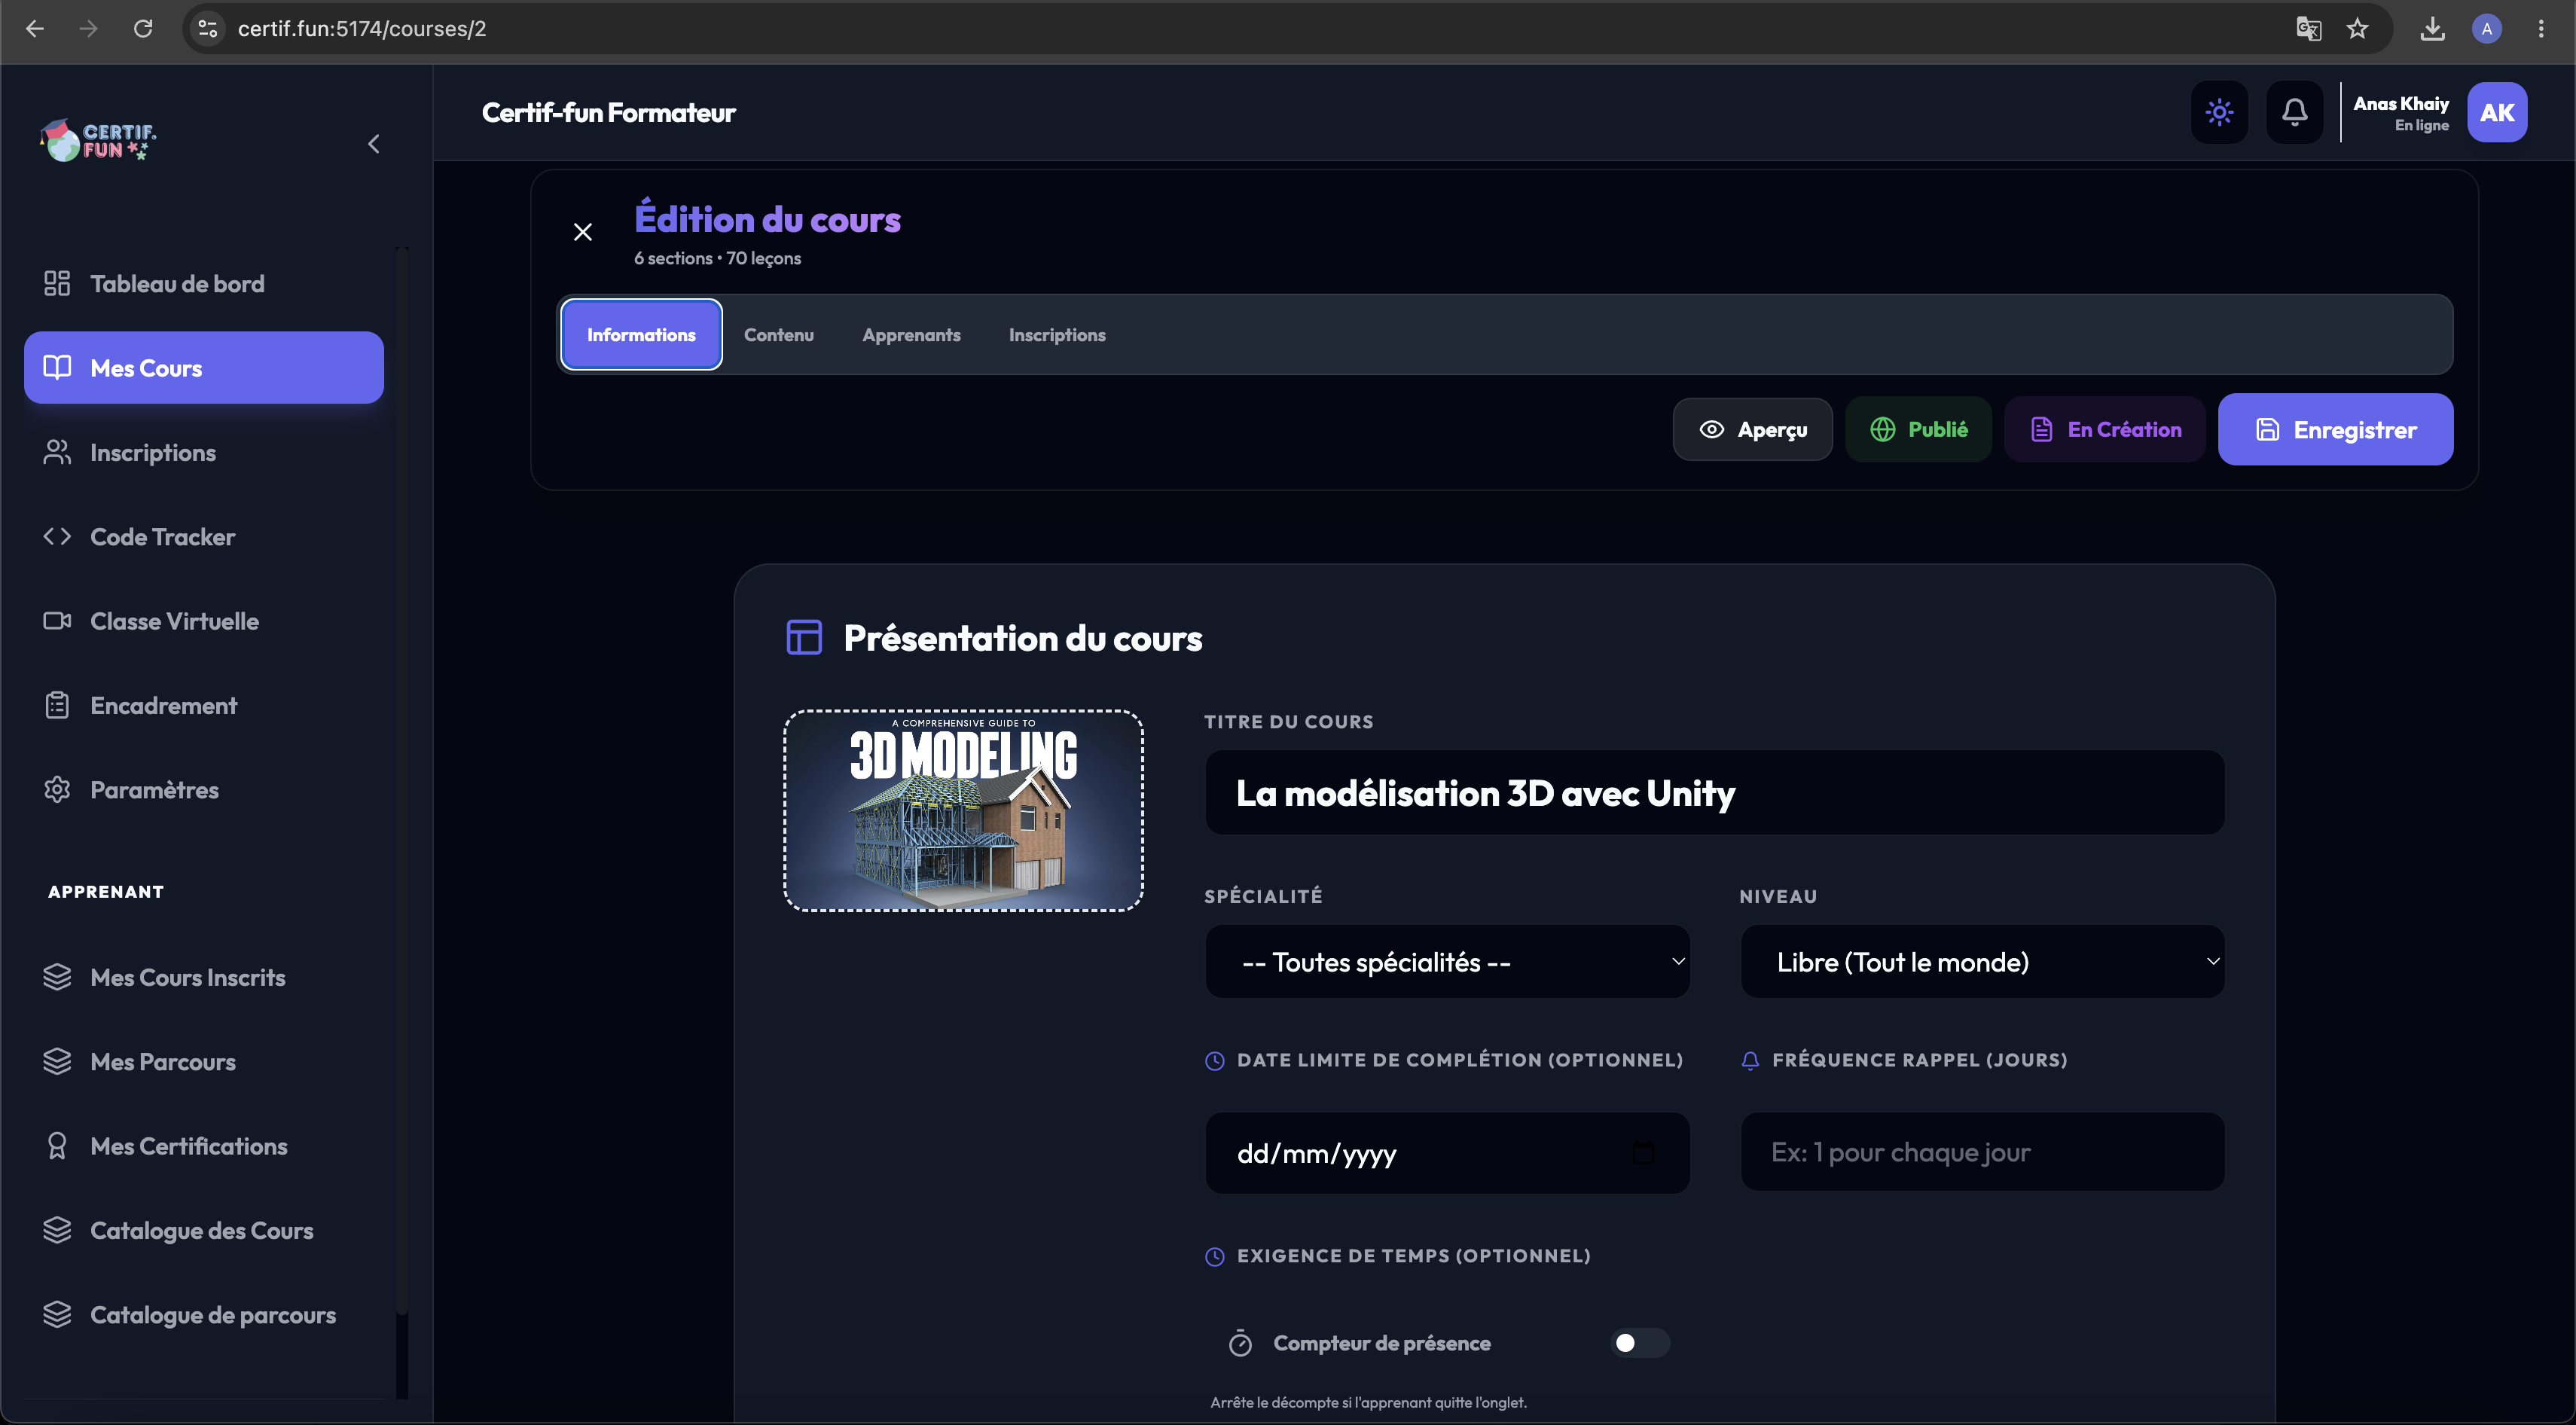
\includegraphics[width=0.98\textwidth]{figures/formateur-2.png}
    \caption{Liste des cours du formateur}
    \label{fig:formateur2}
\end{figure}

Lors de la création d'un nouveau cours (Figure~\ref{fig:formateur3}), le formateur peut structurer son cours en sections et en leçons. Ces leçons peuvent intégrer divers types de contenus tels que des vidéos, du texte, des images ou des quiz.
\begin{figure}[H]
    \centering
    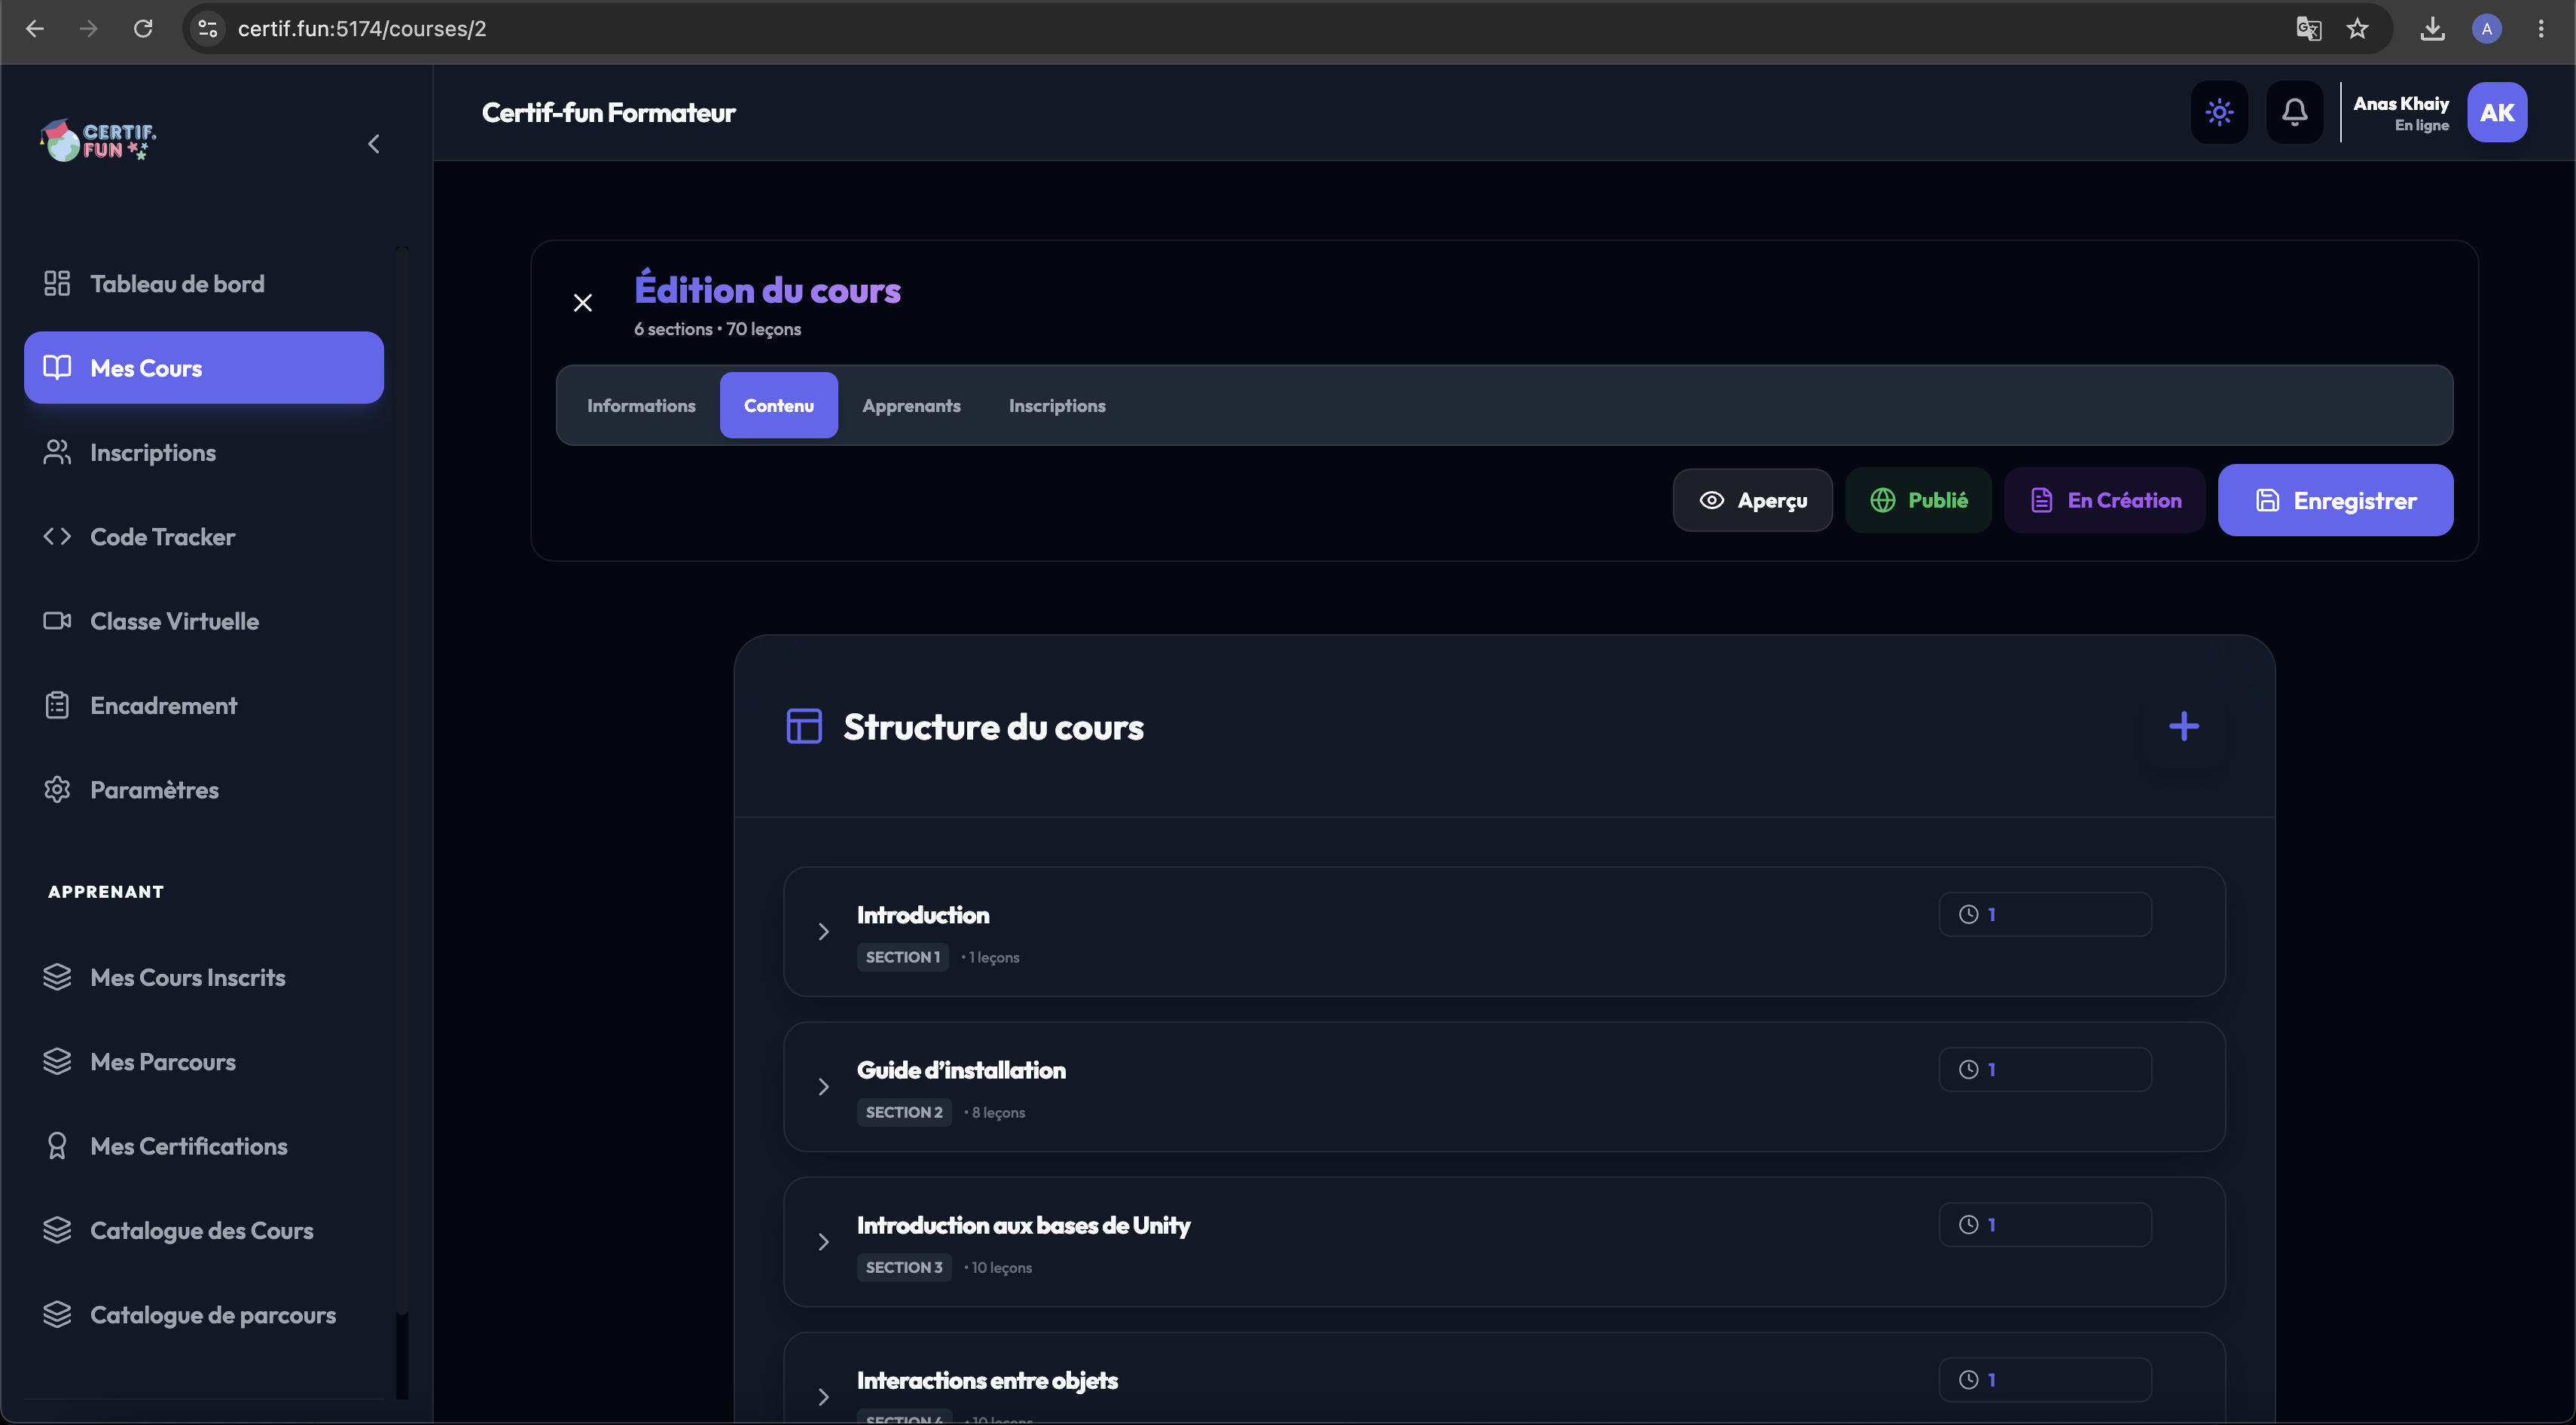
\includegraphics[width=0.98\textwidth]{figures/formateur-3.png}
    \caption{Formulaire de création d'un nouveau cours}
    \label{fig:formateur3}
\end{figure}

L'interface de suivi (Figure~\ref{fig:formateur4}) permet au formateur de visualiser la progression détaillée de chaque étudiant au sein de la formation.
\begin{figure}[H]
    \centering
    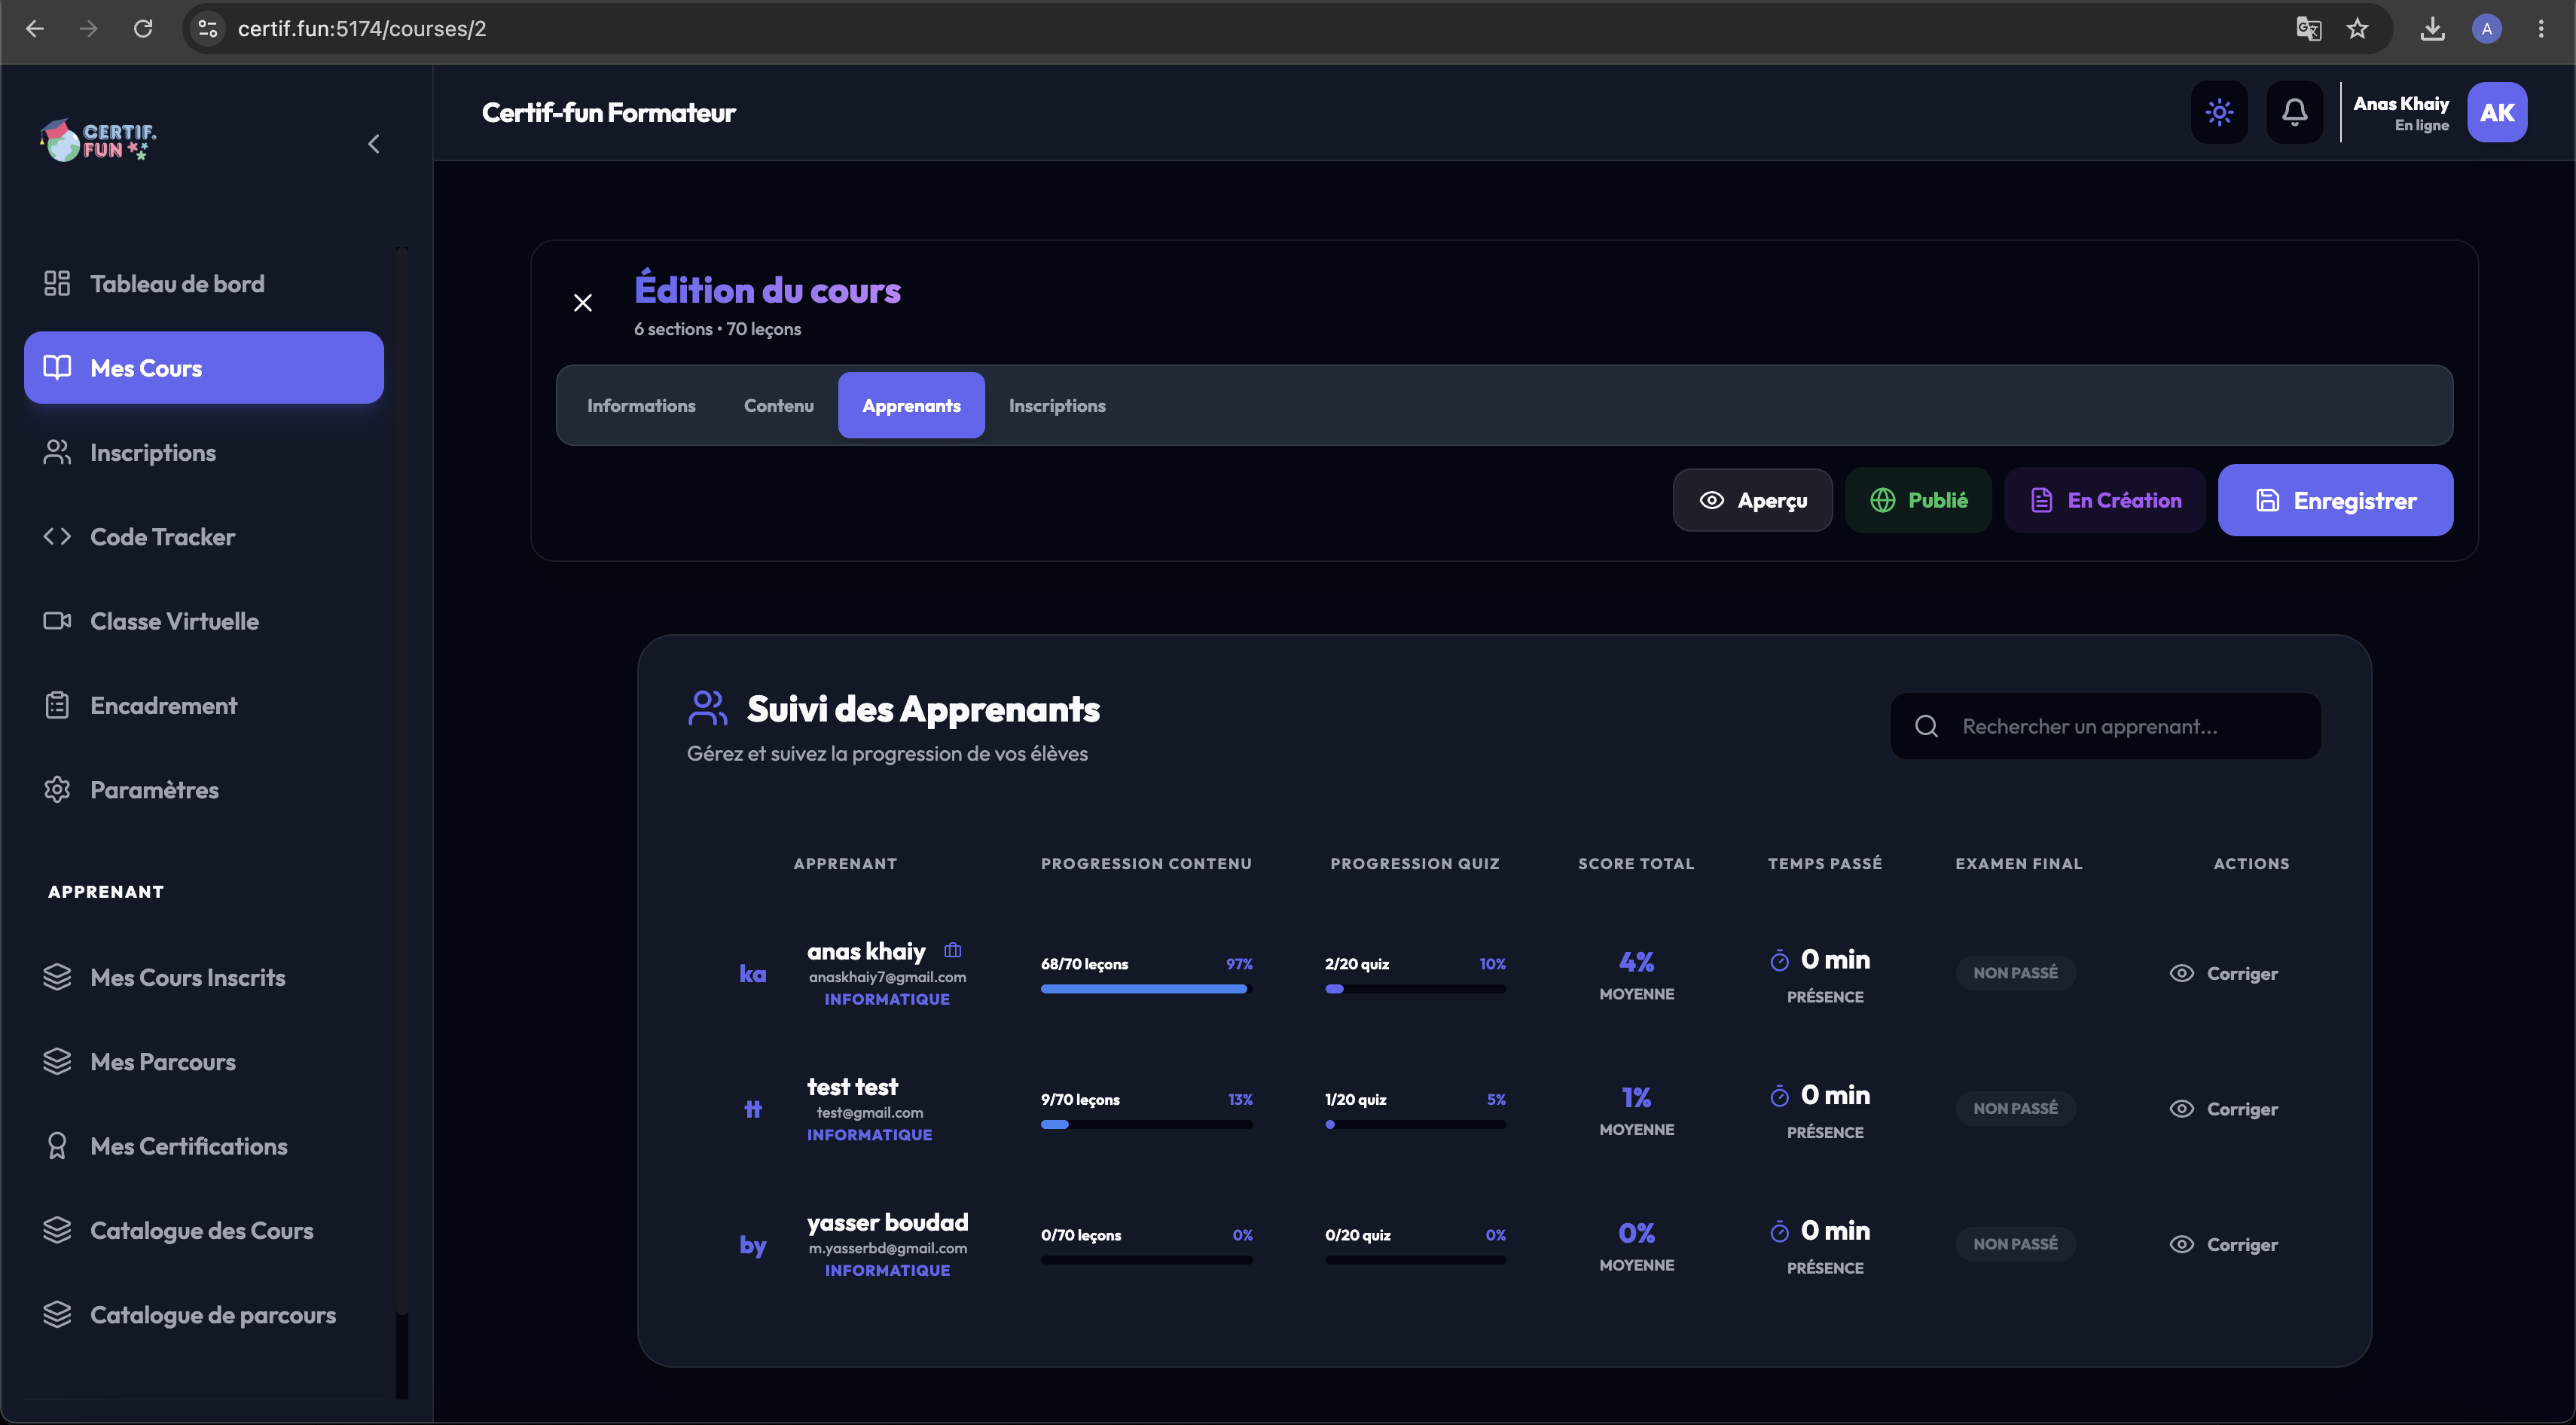
\includegraphics[width=0.98\textwidth]{figures/formateur-4.png}
    \caption{Éditeur de contenu du cours}
    \label{fig:formateur4}
\end{figure}

Le module des inscriptions (Figure~\ref{fig:formateur5}) permet au formateur de gérer directement les inscriptions et les accès de ses apprenants à ses cours.
\begin{figure}[H]
    \centering
    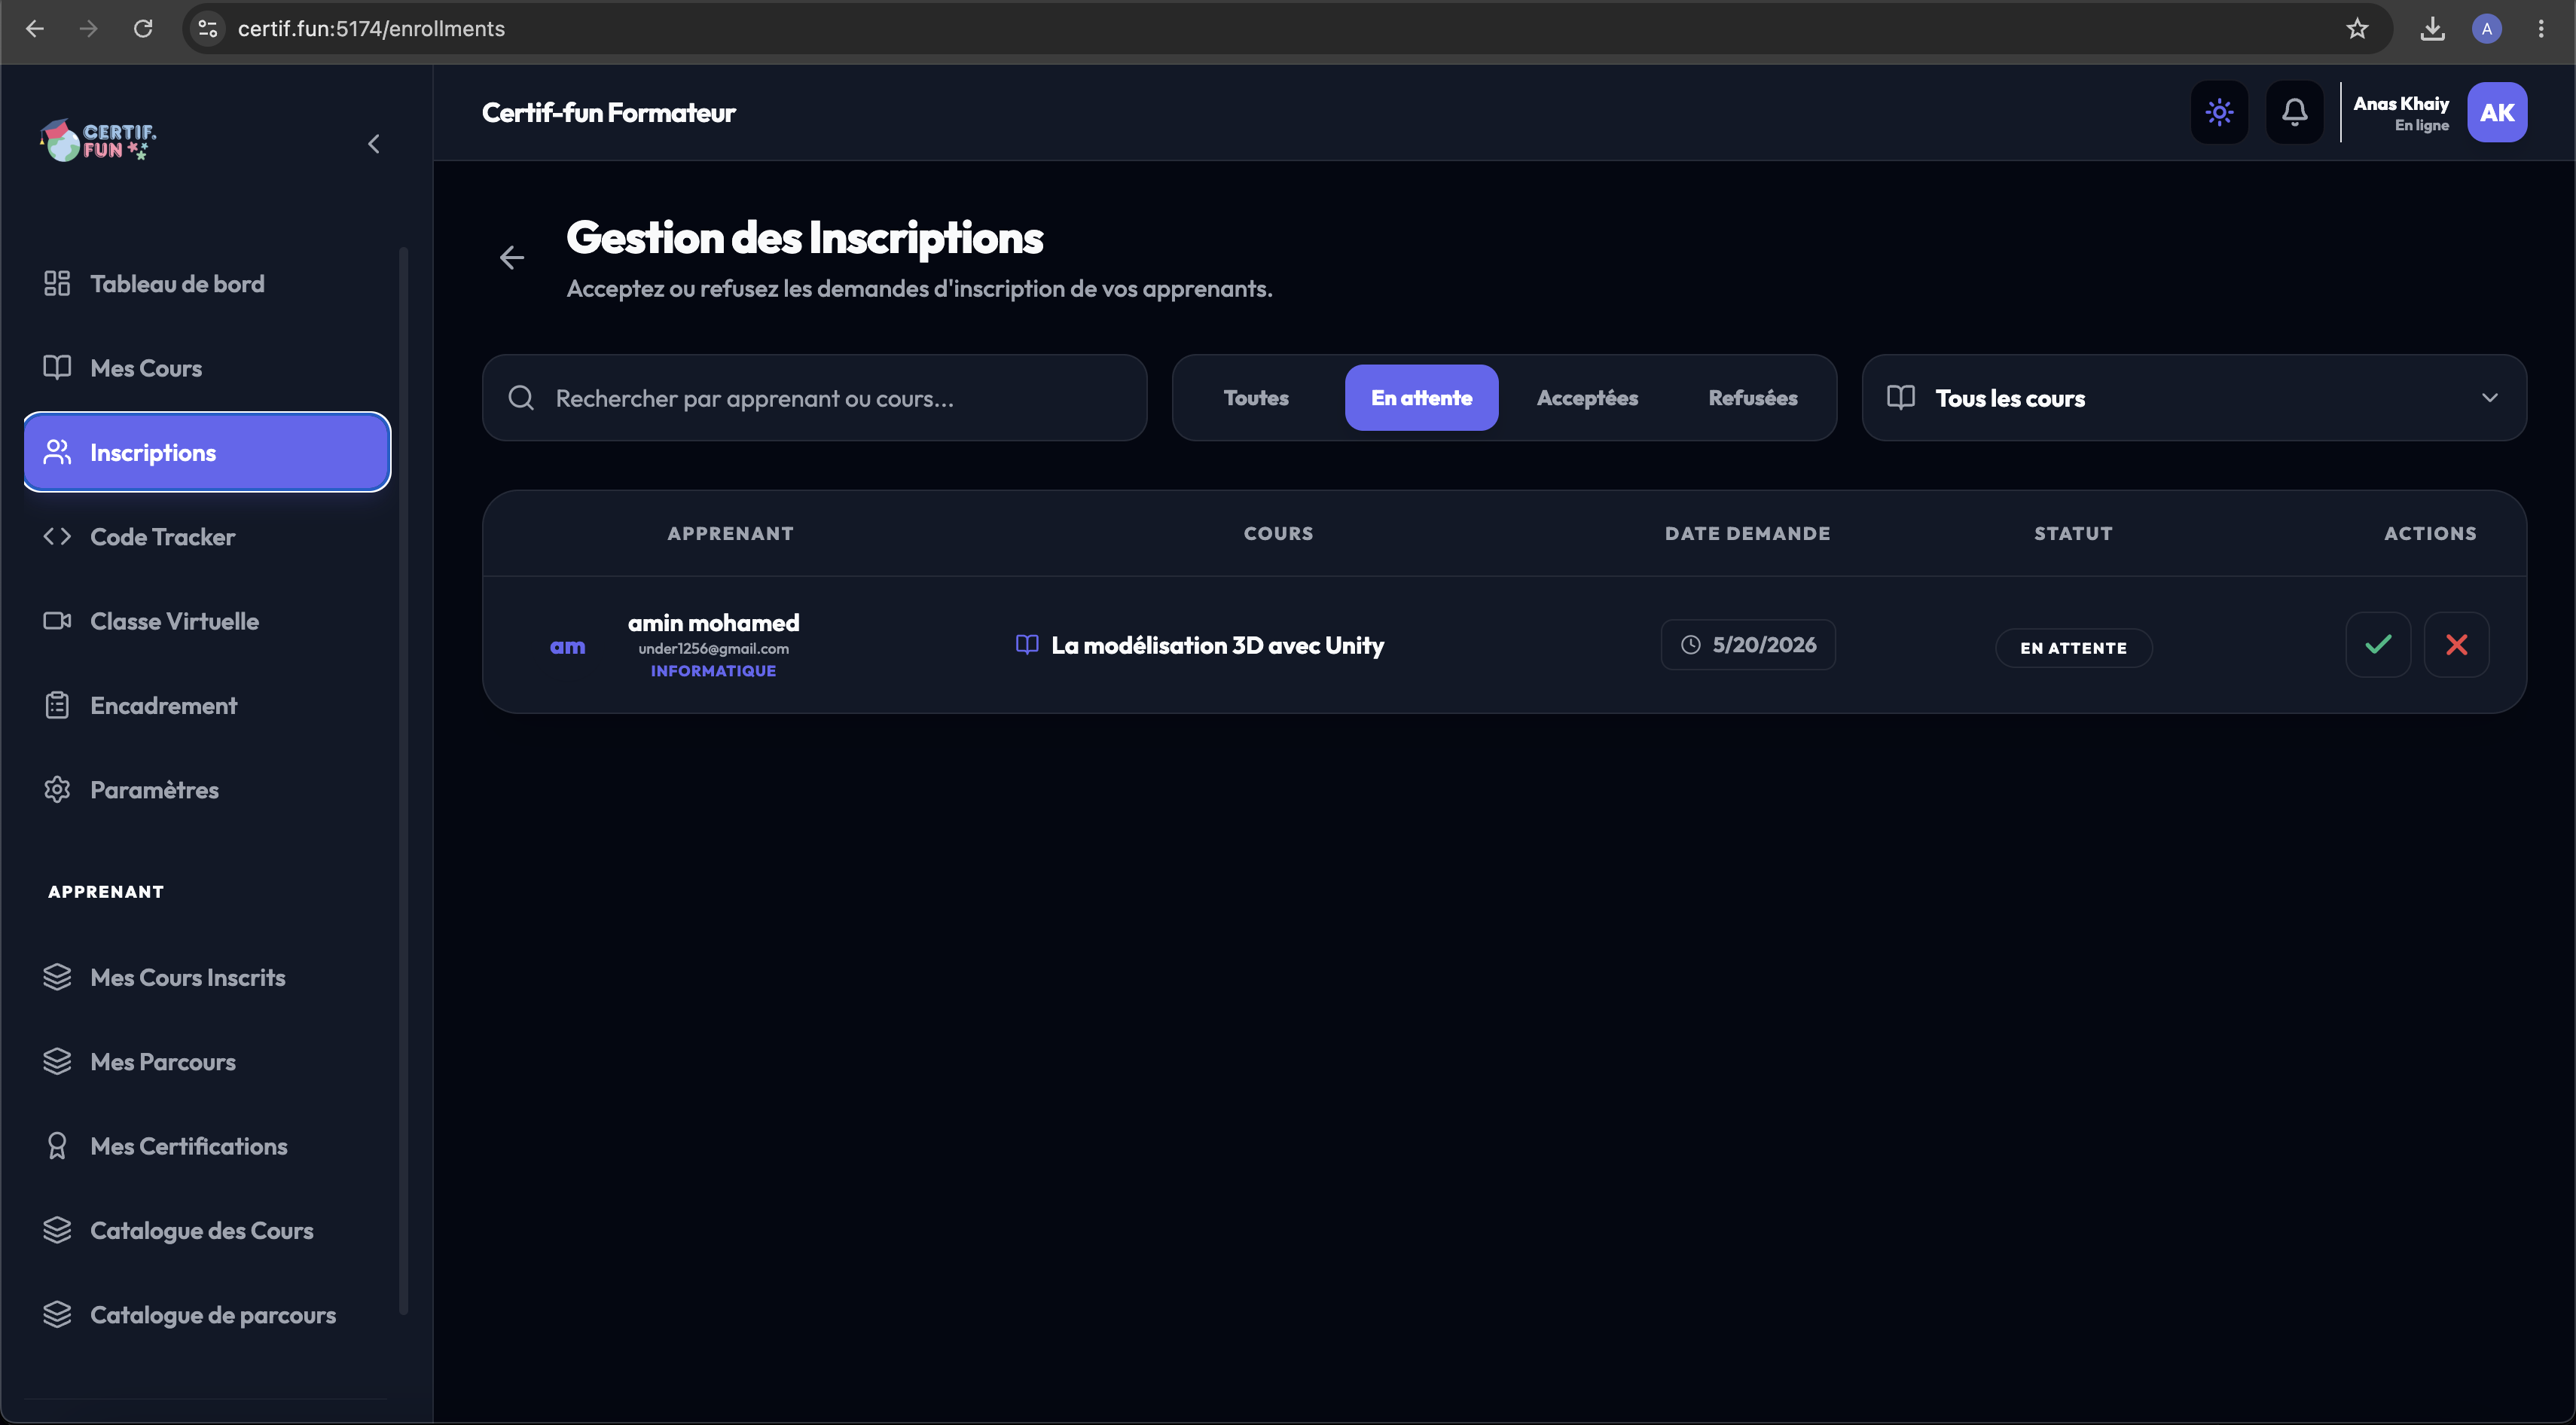
\includegraphics[width=0.98\textwidth]{figures/formateur-5.png}
    \caption{Suivi des inscriptions aux cours du formateur}
    \label{fig:formateur5}
\end{figure}

Pour les matières liées à la programmation, l'outil "Code Tracker" (Figure~\ref{fig:formateur6}) donne la possibilité au formateur de consulter en direct le code écrit par ses étudiants dans les exercices pratiques.
\begin{figure}[H]
    \centering
    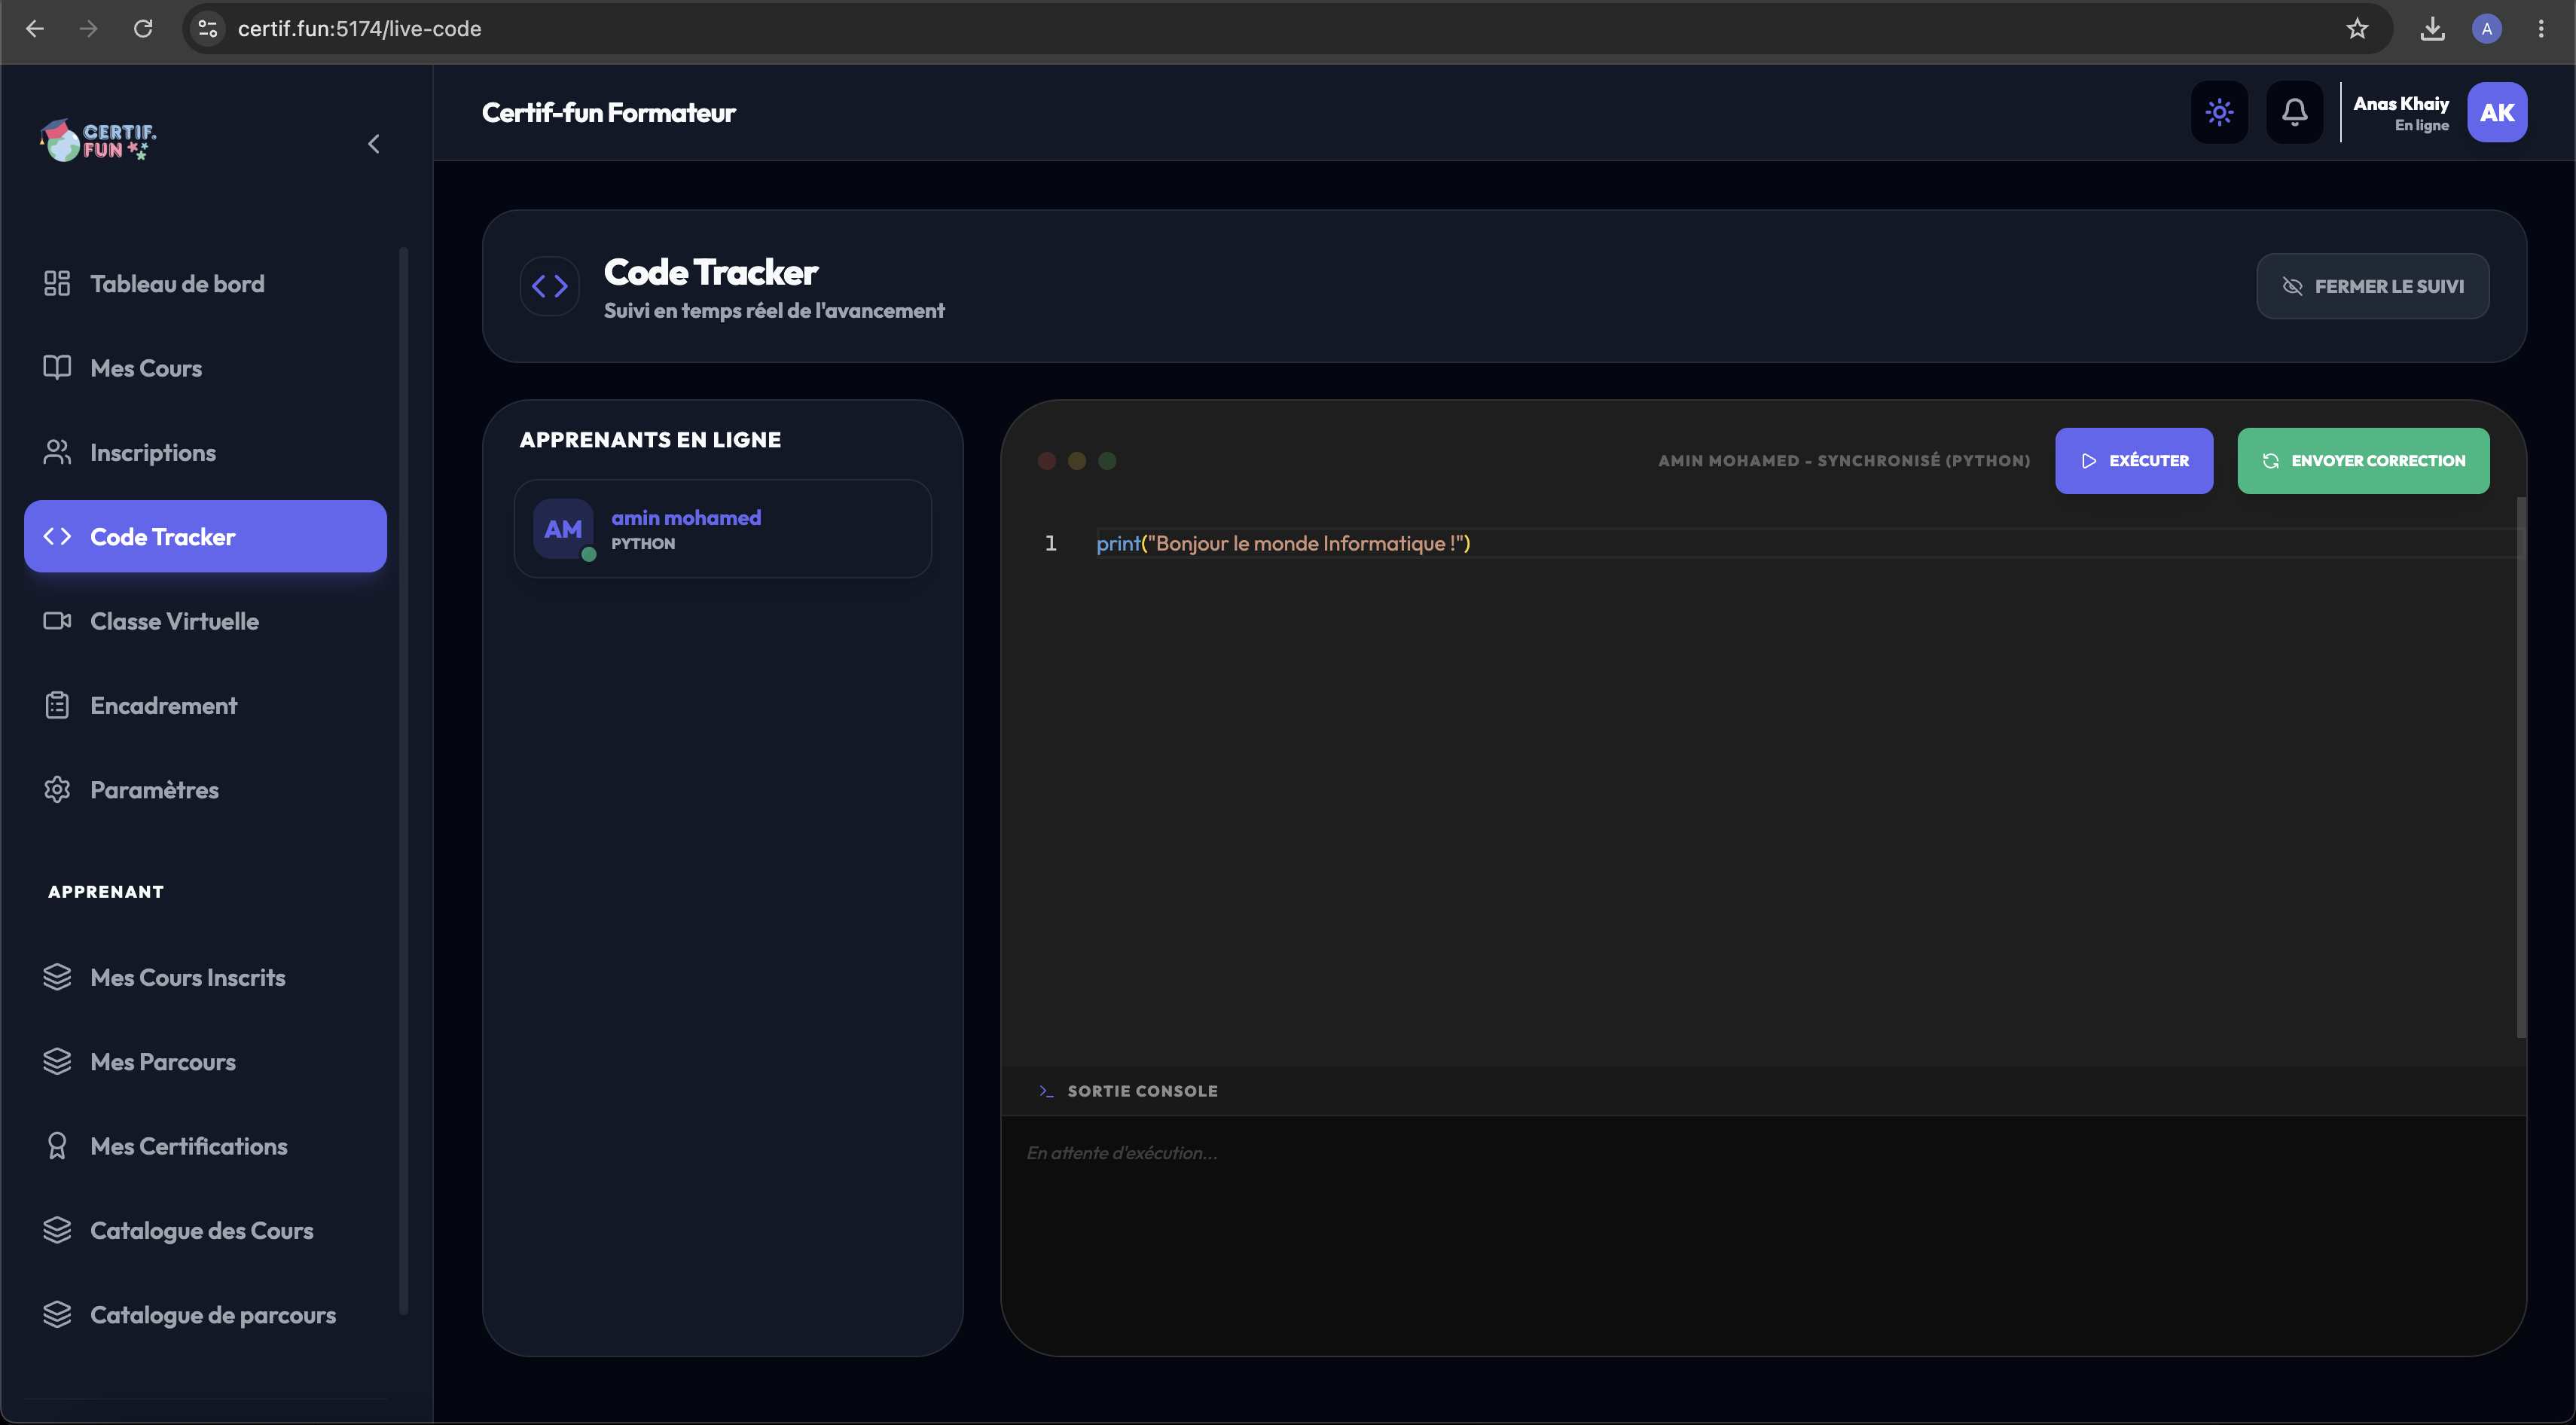
\includegraphics[width=0.98\textwidth]{figures/formateur-6.png}
    \caption{Outil Code Tracker pour les exercices de programmation}
    \label{fig:formateur6}
\end{figure}

Le module "Classe Virtuelle" (Figure~\ref{fig:formateur7}) permet au professeur d'initier une session d'enseignement en visioconférence. Il génère un code de salle (ex. ROOM-EN4SBU1E) qu'il transmet à ses apprenants pour un cours en direct avec partage d'écran et audio.
\begin{figure}[H]
    \centering
    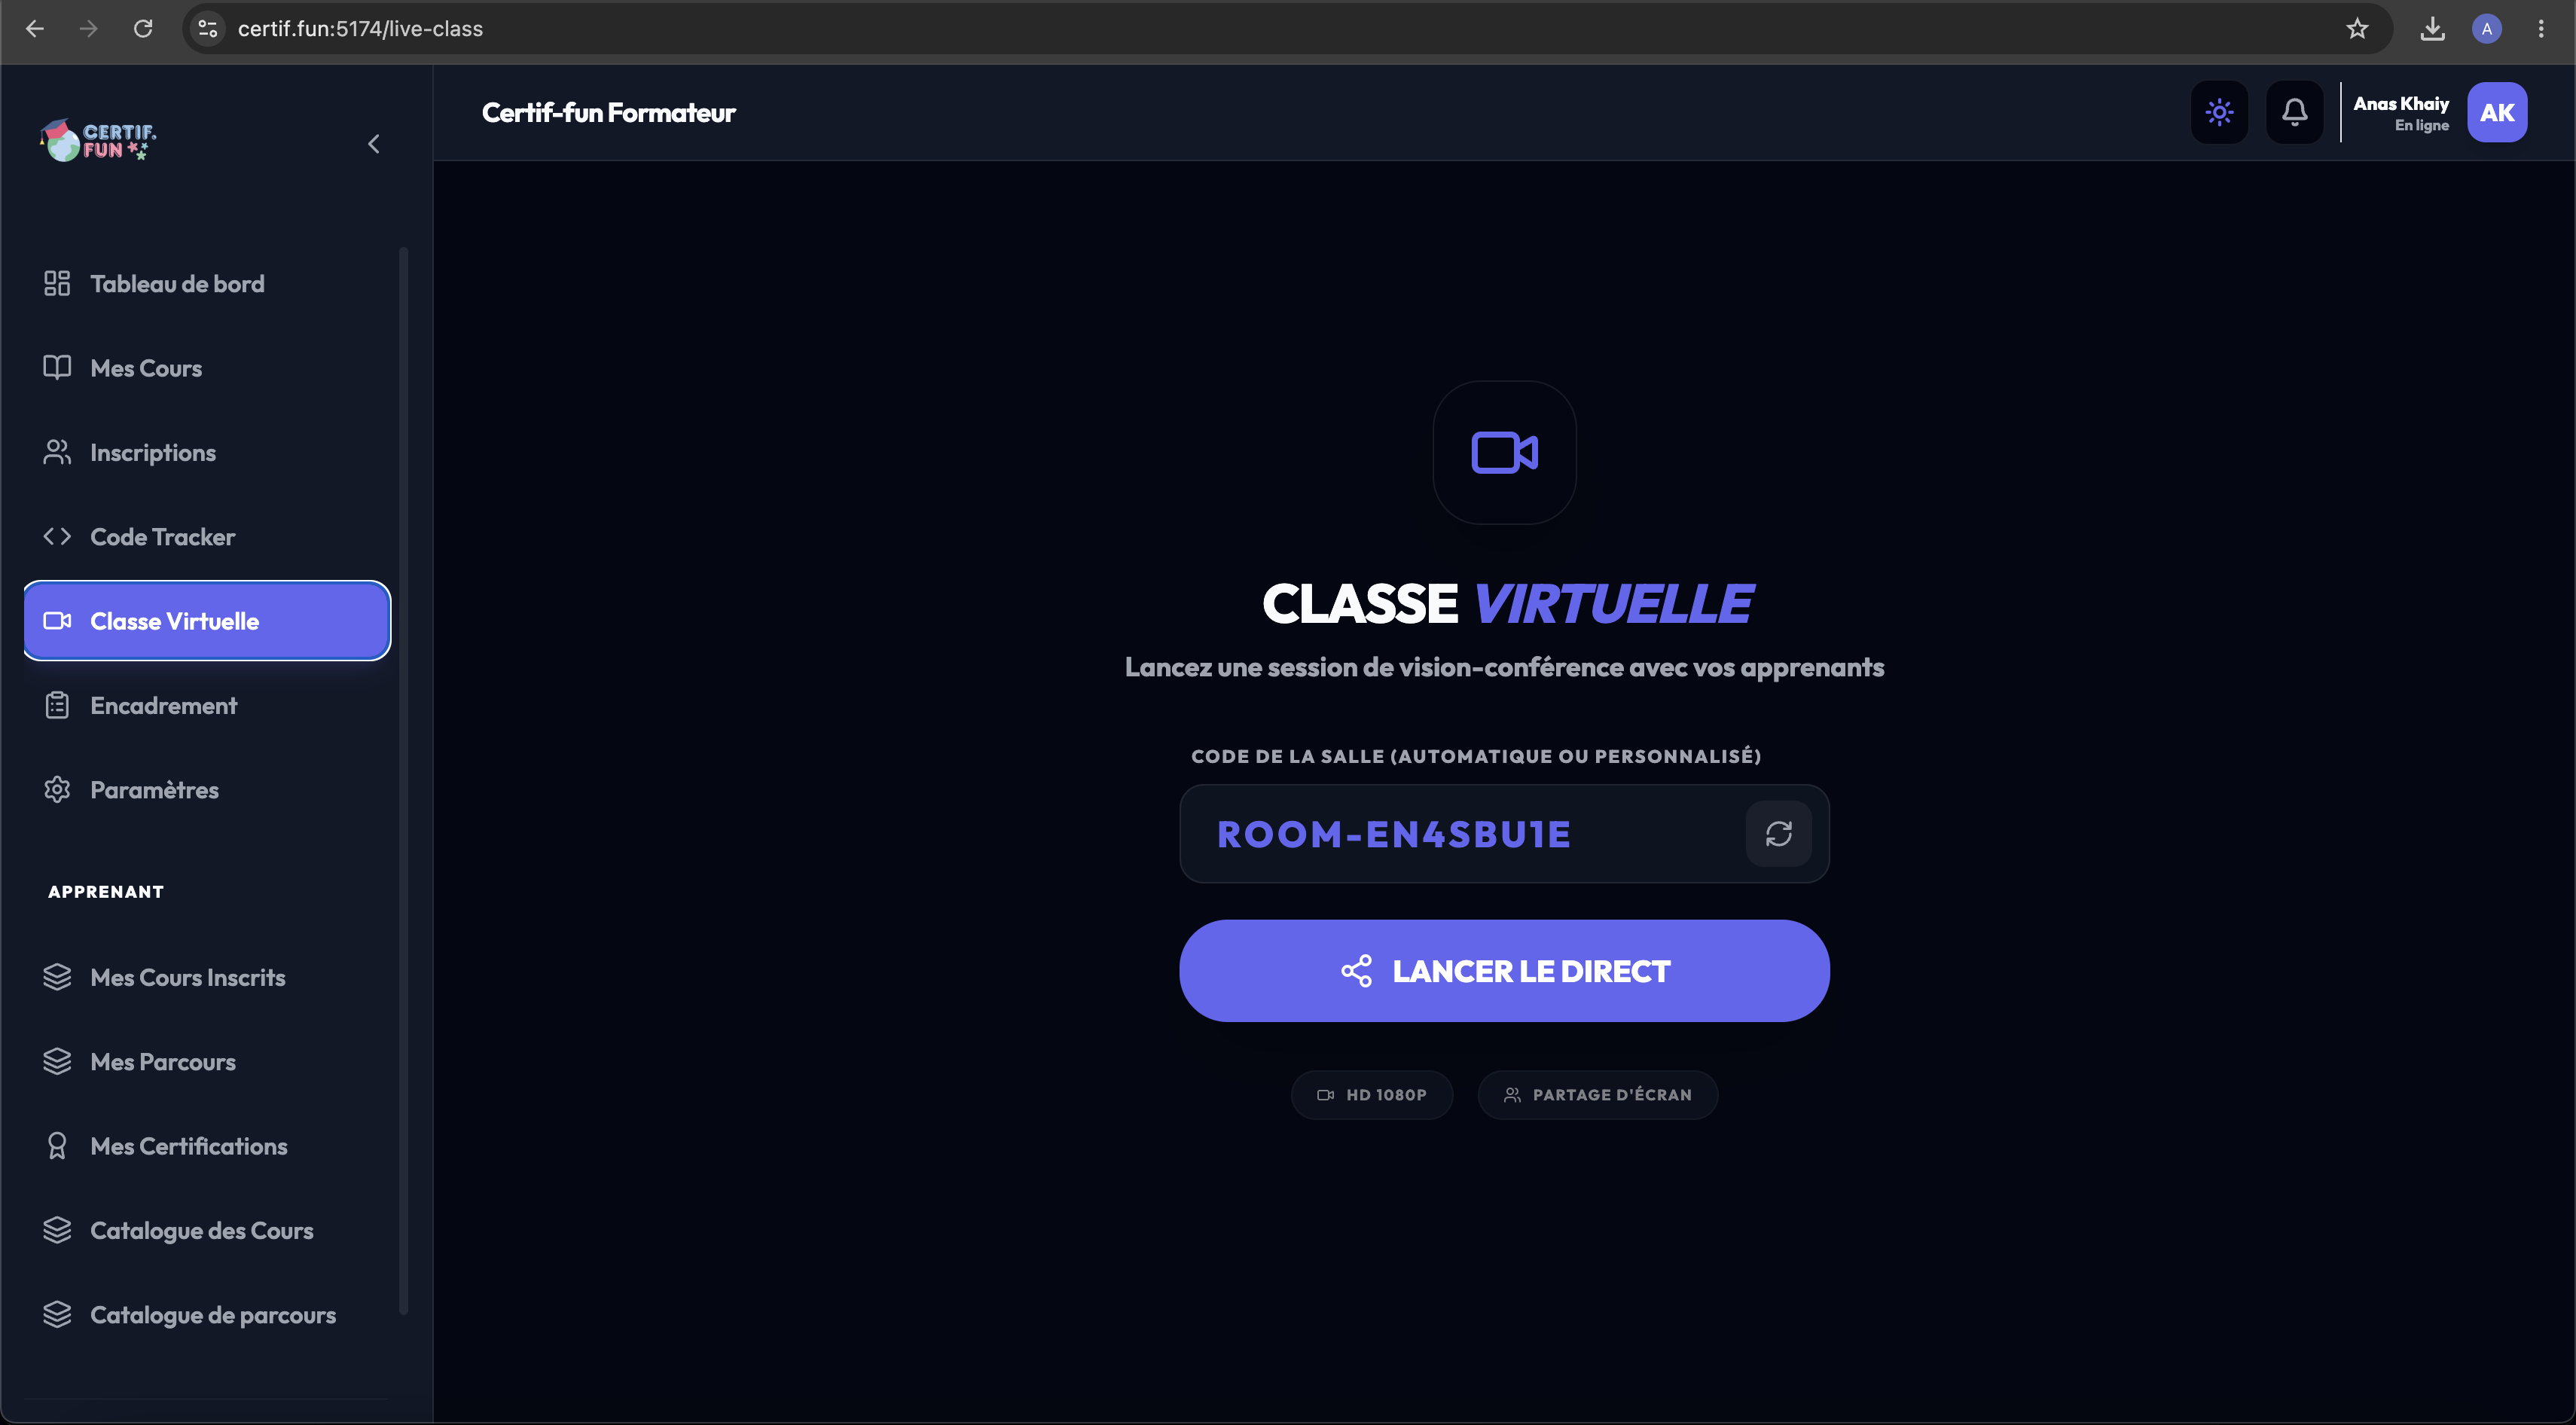
\includegraphics[width=0.98\textwidth]{figures/formateur-7.png}
    \caption{Interface de lancement d'une classe virtuelle}
    \label{fig:formateur7}
\end{figure}

La section "Mon Encadrement" (Figure~\ref{fig:formateur8}) est dédiée au suivi des PFE et des projets longs. Le formateur y suit l'avancement individuel de chaque apprenant encadré et valide ses livrables (rapports, code).
\begin{figure}[H]
    \centering
    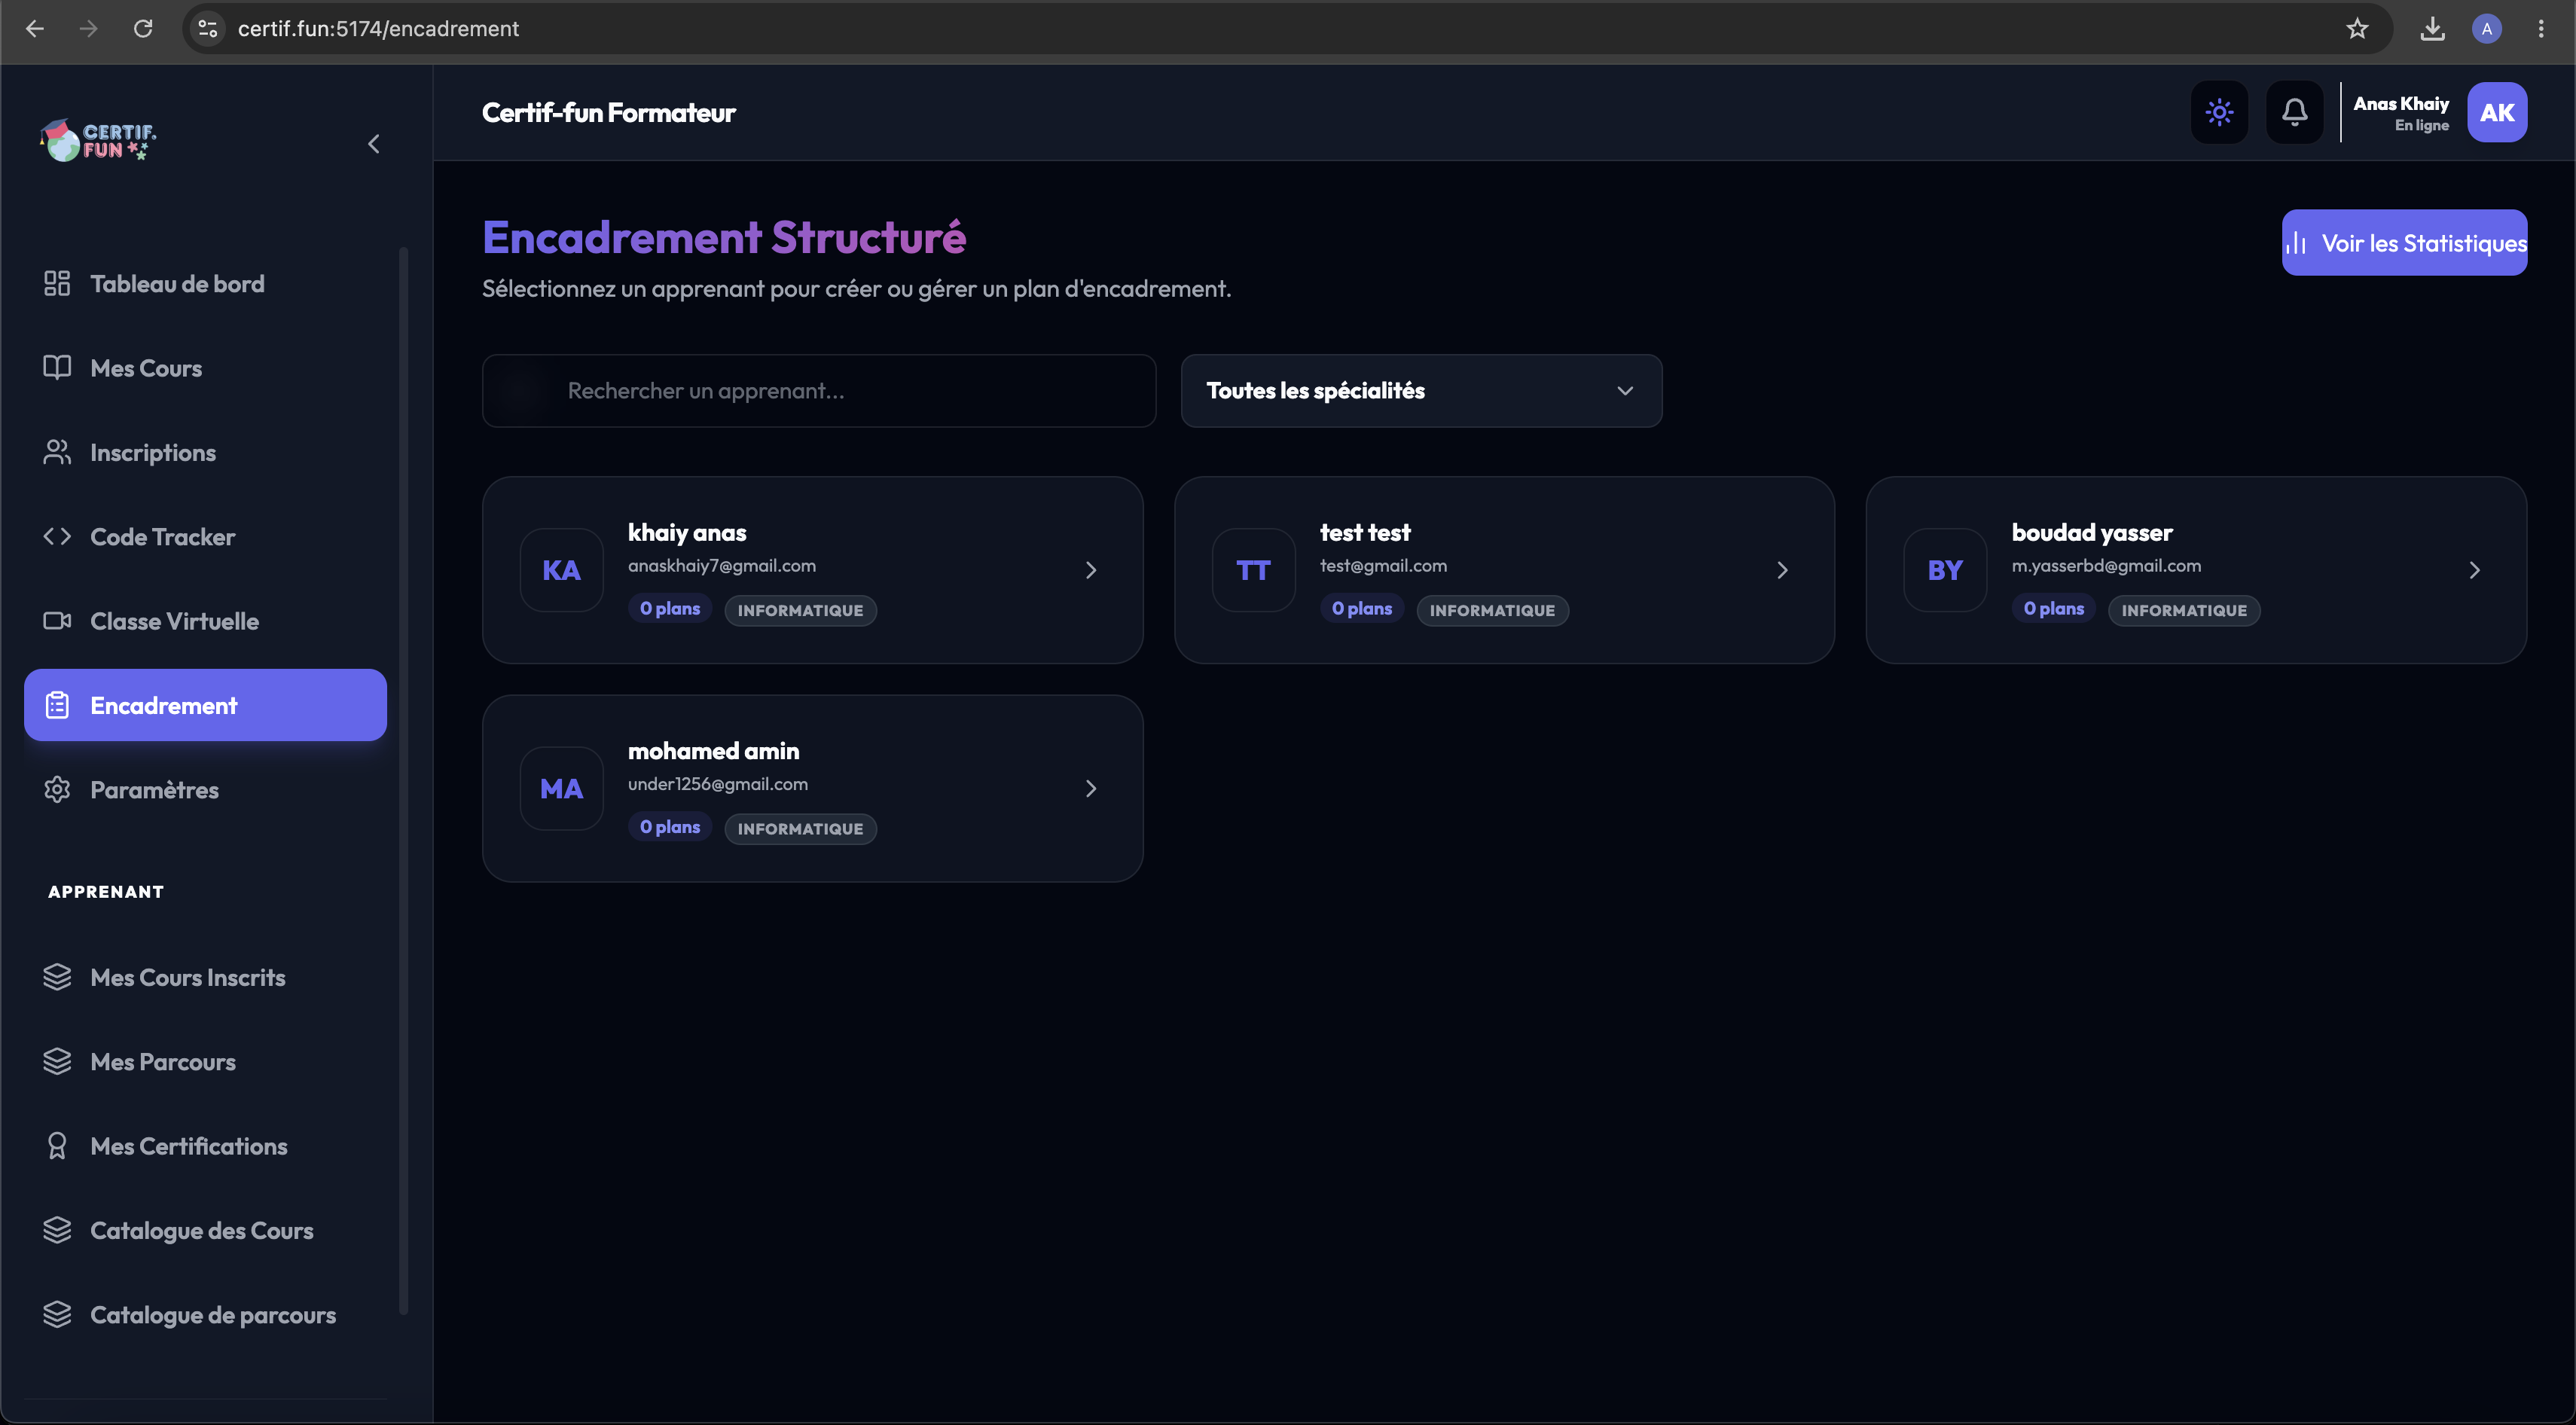
\includegraphics[width=0.98\textwidth]{figures/formateur-8.png}
    \caption{Tableau de bord de l'encadrement structuré}
    \label{fig:formateur8}
\end{figure}

Enfin, le formateur a accès au catalogue des parcours (Figure~\ref{fig:formateur9}), ce qui lui permet de consulter des parcours contenant plusieurs cours afin de se perfectionner via des master classes.
\begin{figure}[H]
    \centering
    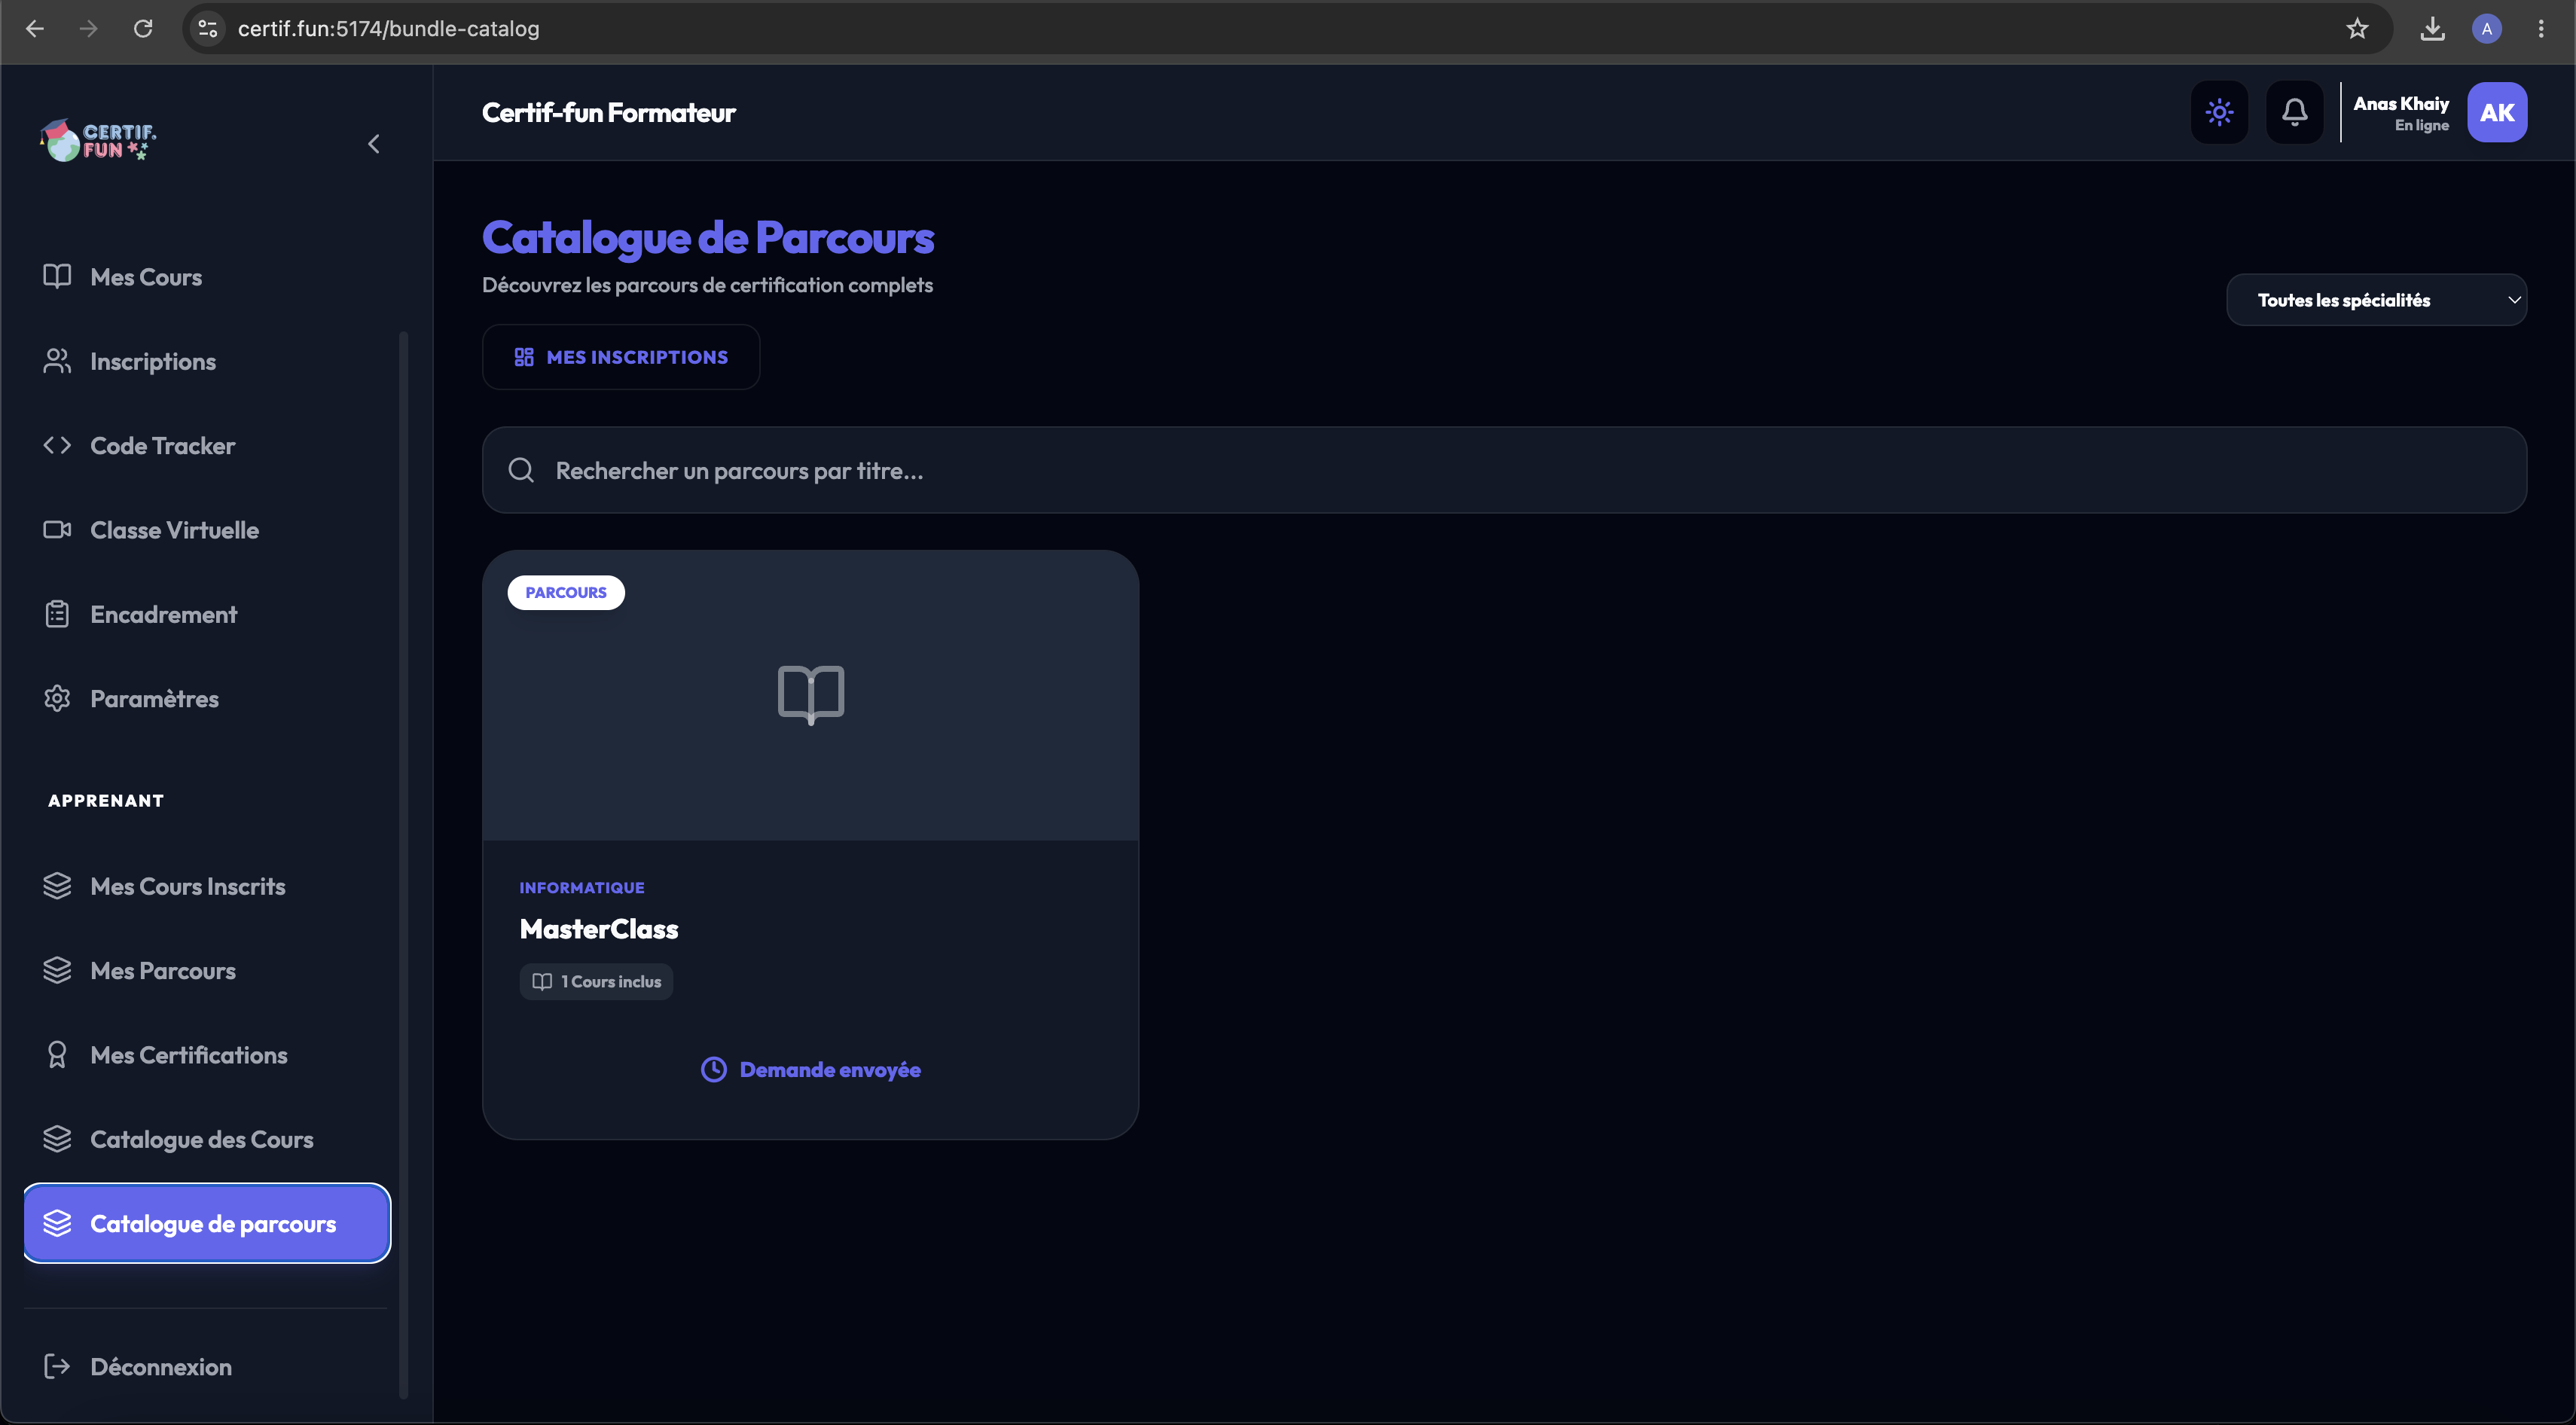
\includegraphics[width=0.98\textwidth]{figures/formateur-9.png}
    \caption{Catalogue global des parcours de certification}
    \label{fig:formateur9}
\end{figure}

Le module de configuration de l'examen final (Figure~\ref{fig:formateur10}) permet au formateur de définir la structure du quiz. Le pool de questions est généré à partir de la masse horaire pour chaque section. Il peut configurer chaque chapitre (section) en spécifiant le poids en pourcentage et le nombre de questions à tirer aléatoirement parmi celles disponibles. Le bilan total affiche le nombre total de questions sélectionnées.
\begin{figure}[H]
    \centering
    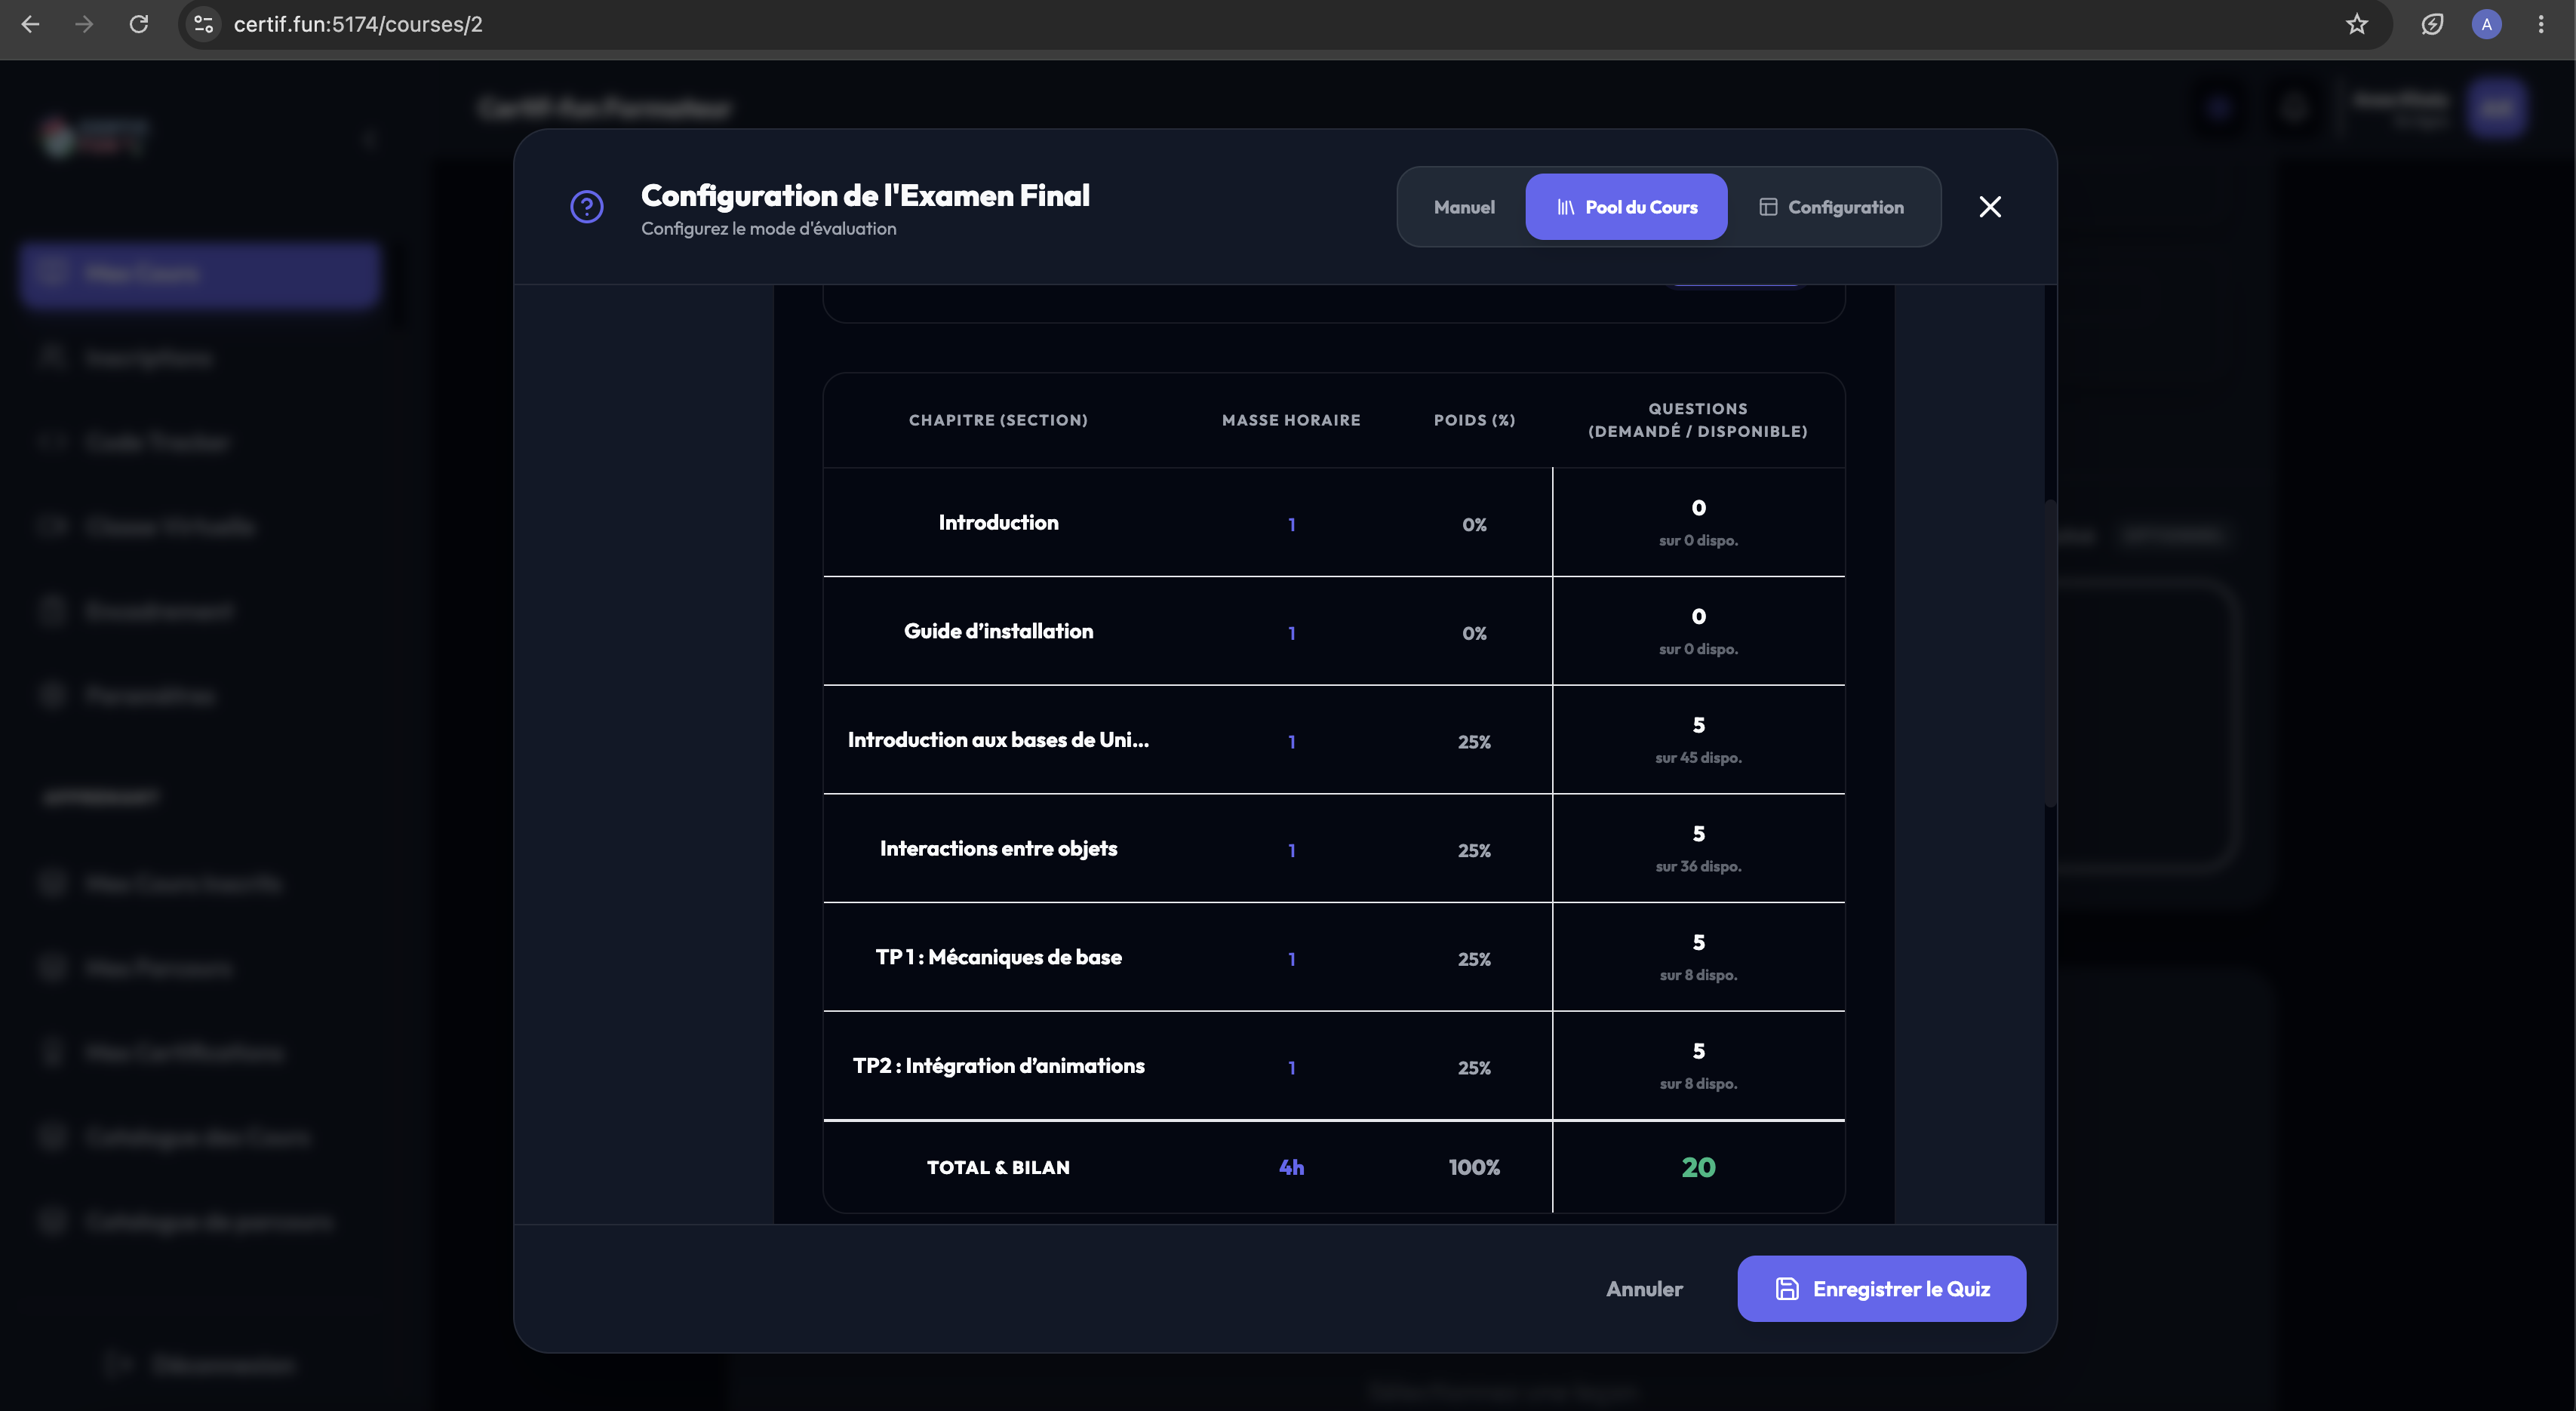
\includegraphics[width=0.98\textwidth]{figures/formateur-10.png}
    \caption{Configuration de l'examen final -- Pool du Cours}
    \label{fig:formateur10}
\end{figure}

La figure~\ref{fig:formateur11} illustre l'onglet de configuration avancée offrant au formateur les contrôles de surveillance par IA (Caméra). Lorsqu'elle est activée, l'apprenant doit obligatoirement utiliser sa caméra pendant l'examen. Le formateur peut activer ou désactiver individuellement les contrôles de détection : détection de téléphone portable, présence de plusieurs personnes, objets interdits (tablettes, écrans) et regard détourné. La section des contrôles anti-triche (Navigateur) permet également de détecter les changements d'onglet pendant l'examen.
\begin{figure}[H]
    \centering
    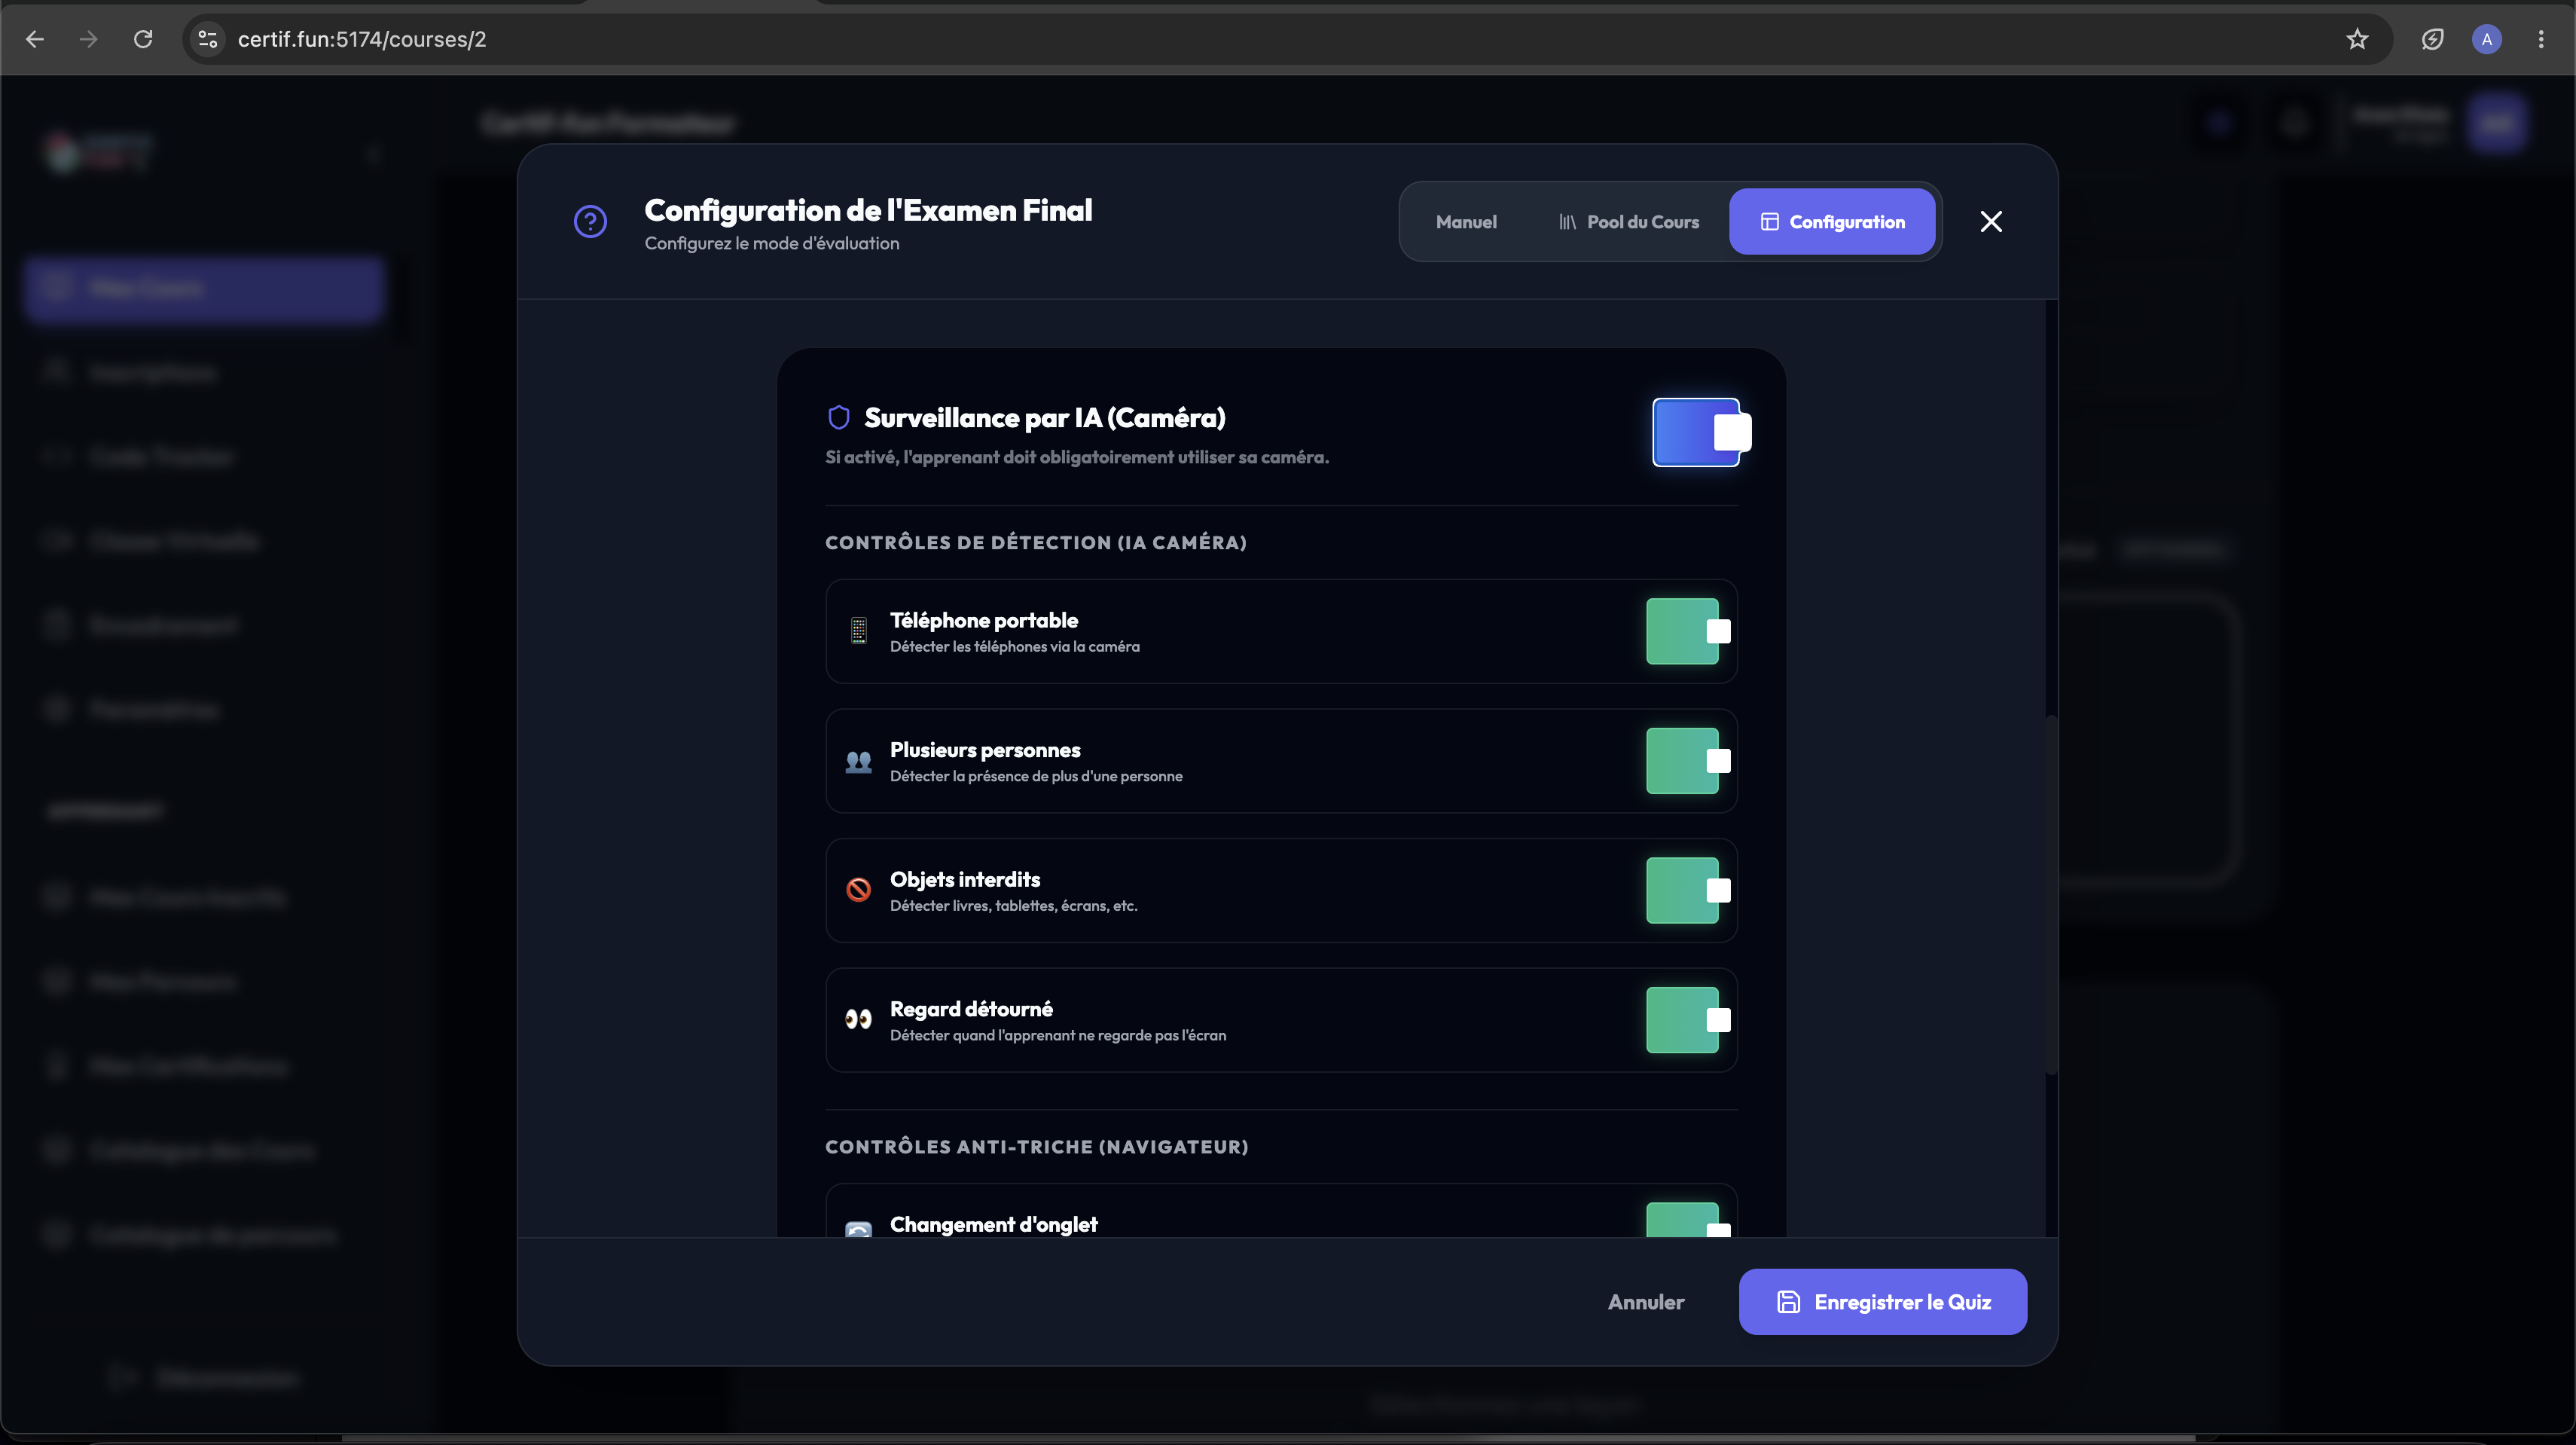
\includegraphics[width=0.98\textwidth]{figures/formateur-11.png}
    \caption{Configuration de la surveillance par IA et contrôles anti-triche}
    \label{fig:formateur11}
\end{figure}

\subsubsection{Portail Apprenant}
L'espace Apprenant vise à offrir une expérience d'apprentissage simple, organisée et efficace.

Le tableau de bord personnel (Figure~\ref{fig:apprenant1}) accueille l'étudiant avec un résumé de sa progression (cours inscrits, terminés, score moyen). Il lui propose un accès rapide pour continuer l'apprentissage et affiche l'historique de ses derniers résultats d'examens.
\begin{figure}[H]
    \centering
    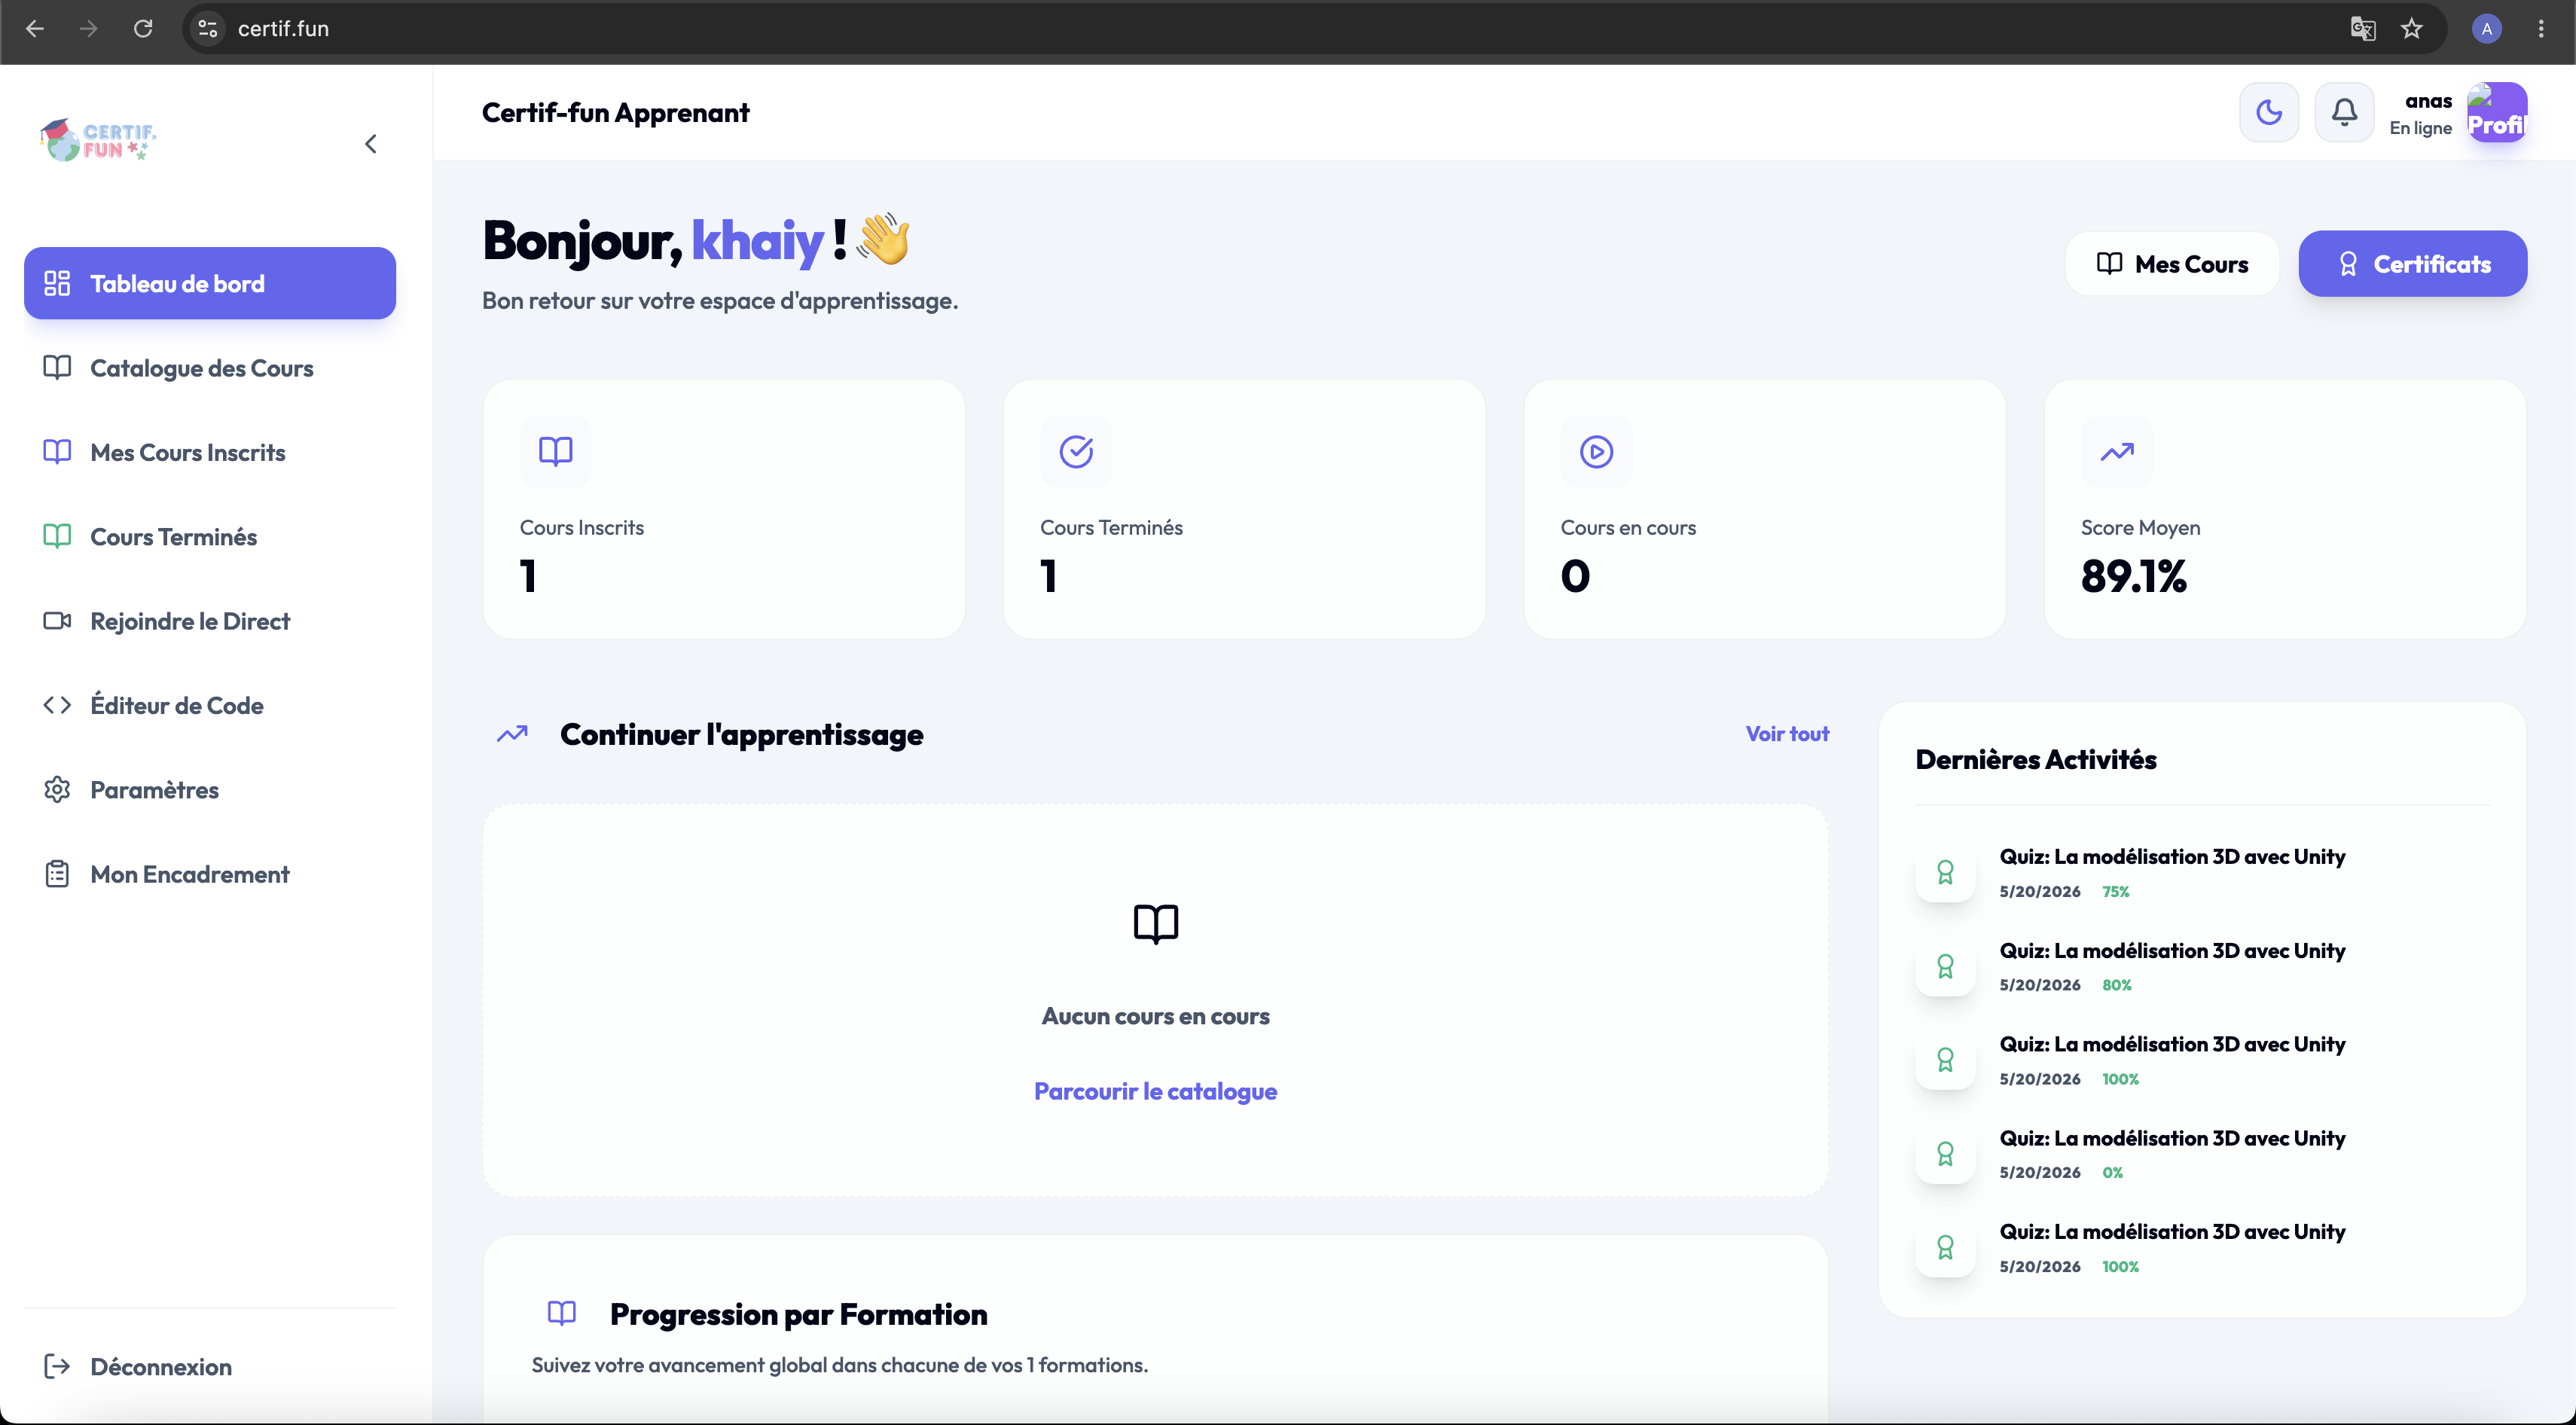
\includegraphics[width=0.98\textwidth]{figures/apprenant-1.png}
    \caption{Tableau de bord de l'Apprenant}
    \label{fig:apprenant1}
\end{figure}

Le catalogue de cours (Figure~\ref{fig:apprenant2}) permet à l'apprenant d'explorer toute l'offre de formation de la plateforme. Grâce à des filtres par catégorie ou niveau, il peut facilement trouver une nouvelle compétence à acquérir et s'y inscrire.
\begin{figure}[H]
    \centering
    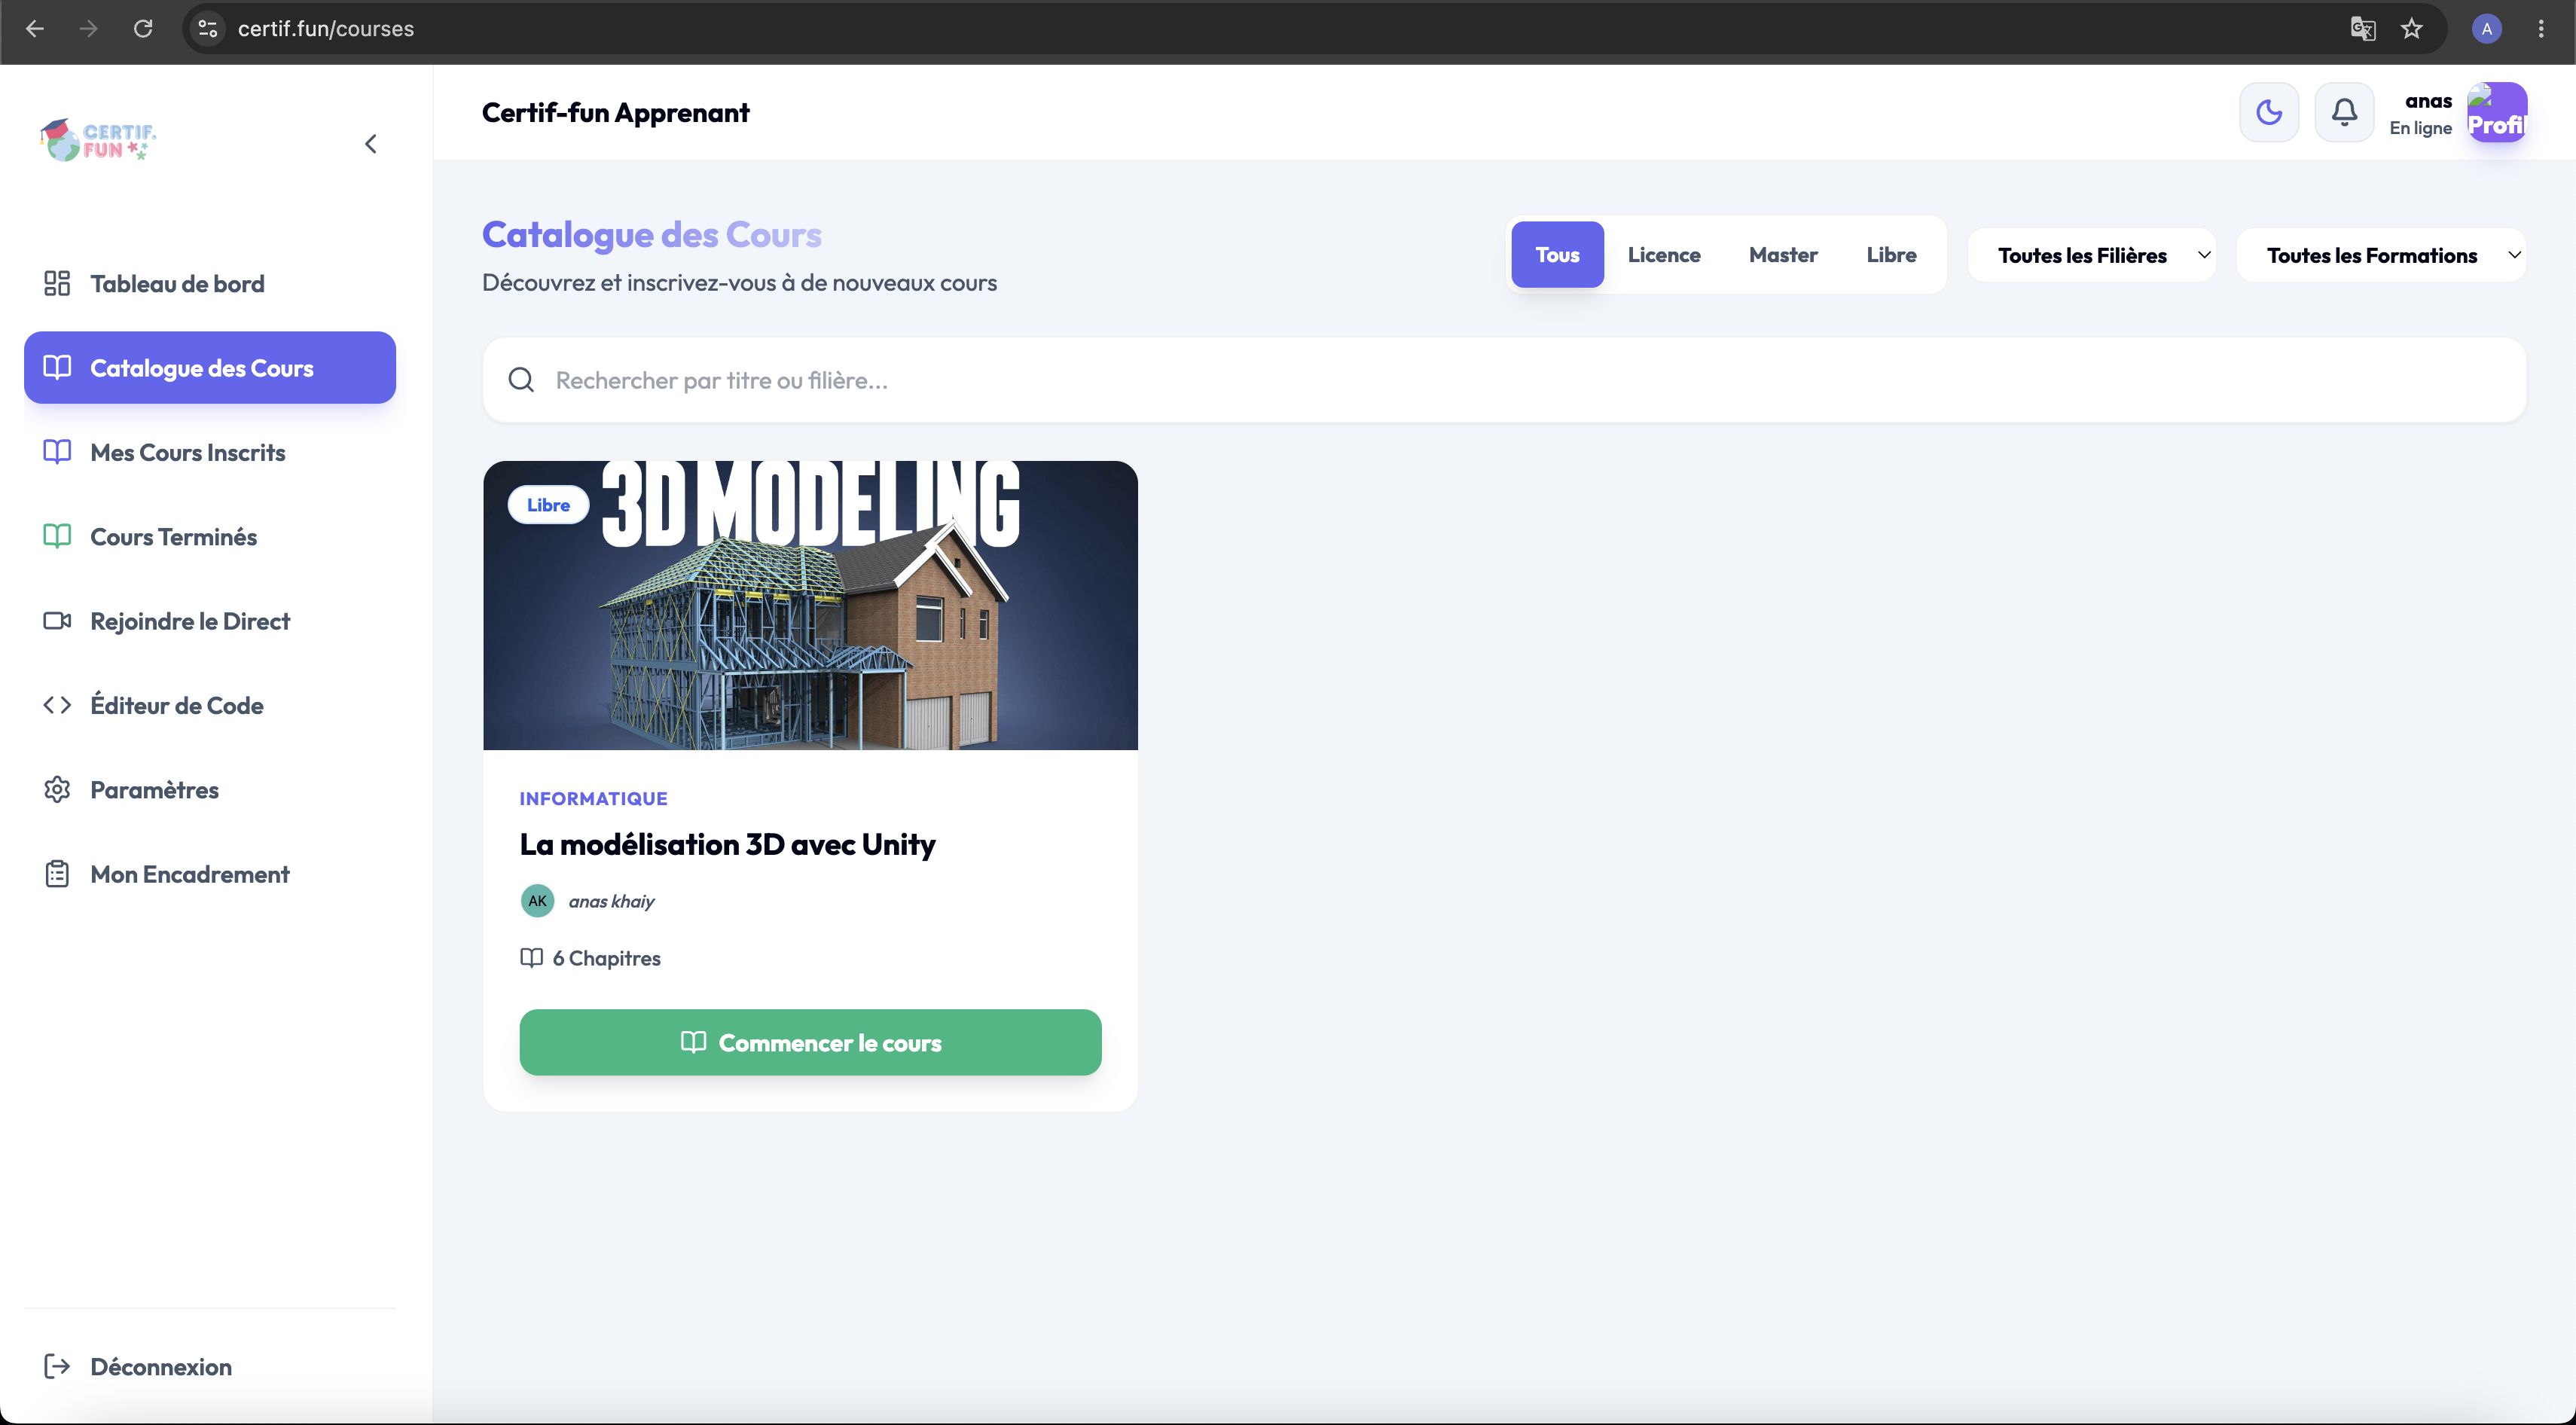
\includegraphics[width=0.98\textwidth]{figures/apprenant-2.png}
    \caption{Catalogue interactif des cours}
    \label{fig:apprenant2}
\end{figure}

Dans la rubrique "Cours Terminés" (Figure~\ref{fig:apprenant3}), l'apprenant retrouve l'ensemble des certificats qu'il a obtenus. Cette vue lui permet de visualiser son diplôme, de l'imprimer ou de le télécharger en version PDF.
\begin{figure}[H]
    \centering
    
\includegraphics[width=0.98\textwidth]{figures/apprenant-3.png}
    \caption{Affichage et impression d'un certificat de réussite}
    \label{fig:apprenant3}
\end{figure}

L'onglet "Rejoindre le Direct" (Figure~\ref{fig:apprenant4}) permet à l'étudiant de se connecter à une classe virtuelle. En renseignant le code fourni par l'enseignant, il entre directement dans la salle de visioconférence pour suivre son cours en temps réel.
\begin{figure}[H]
    \centering
    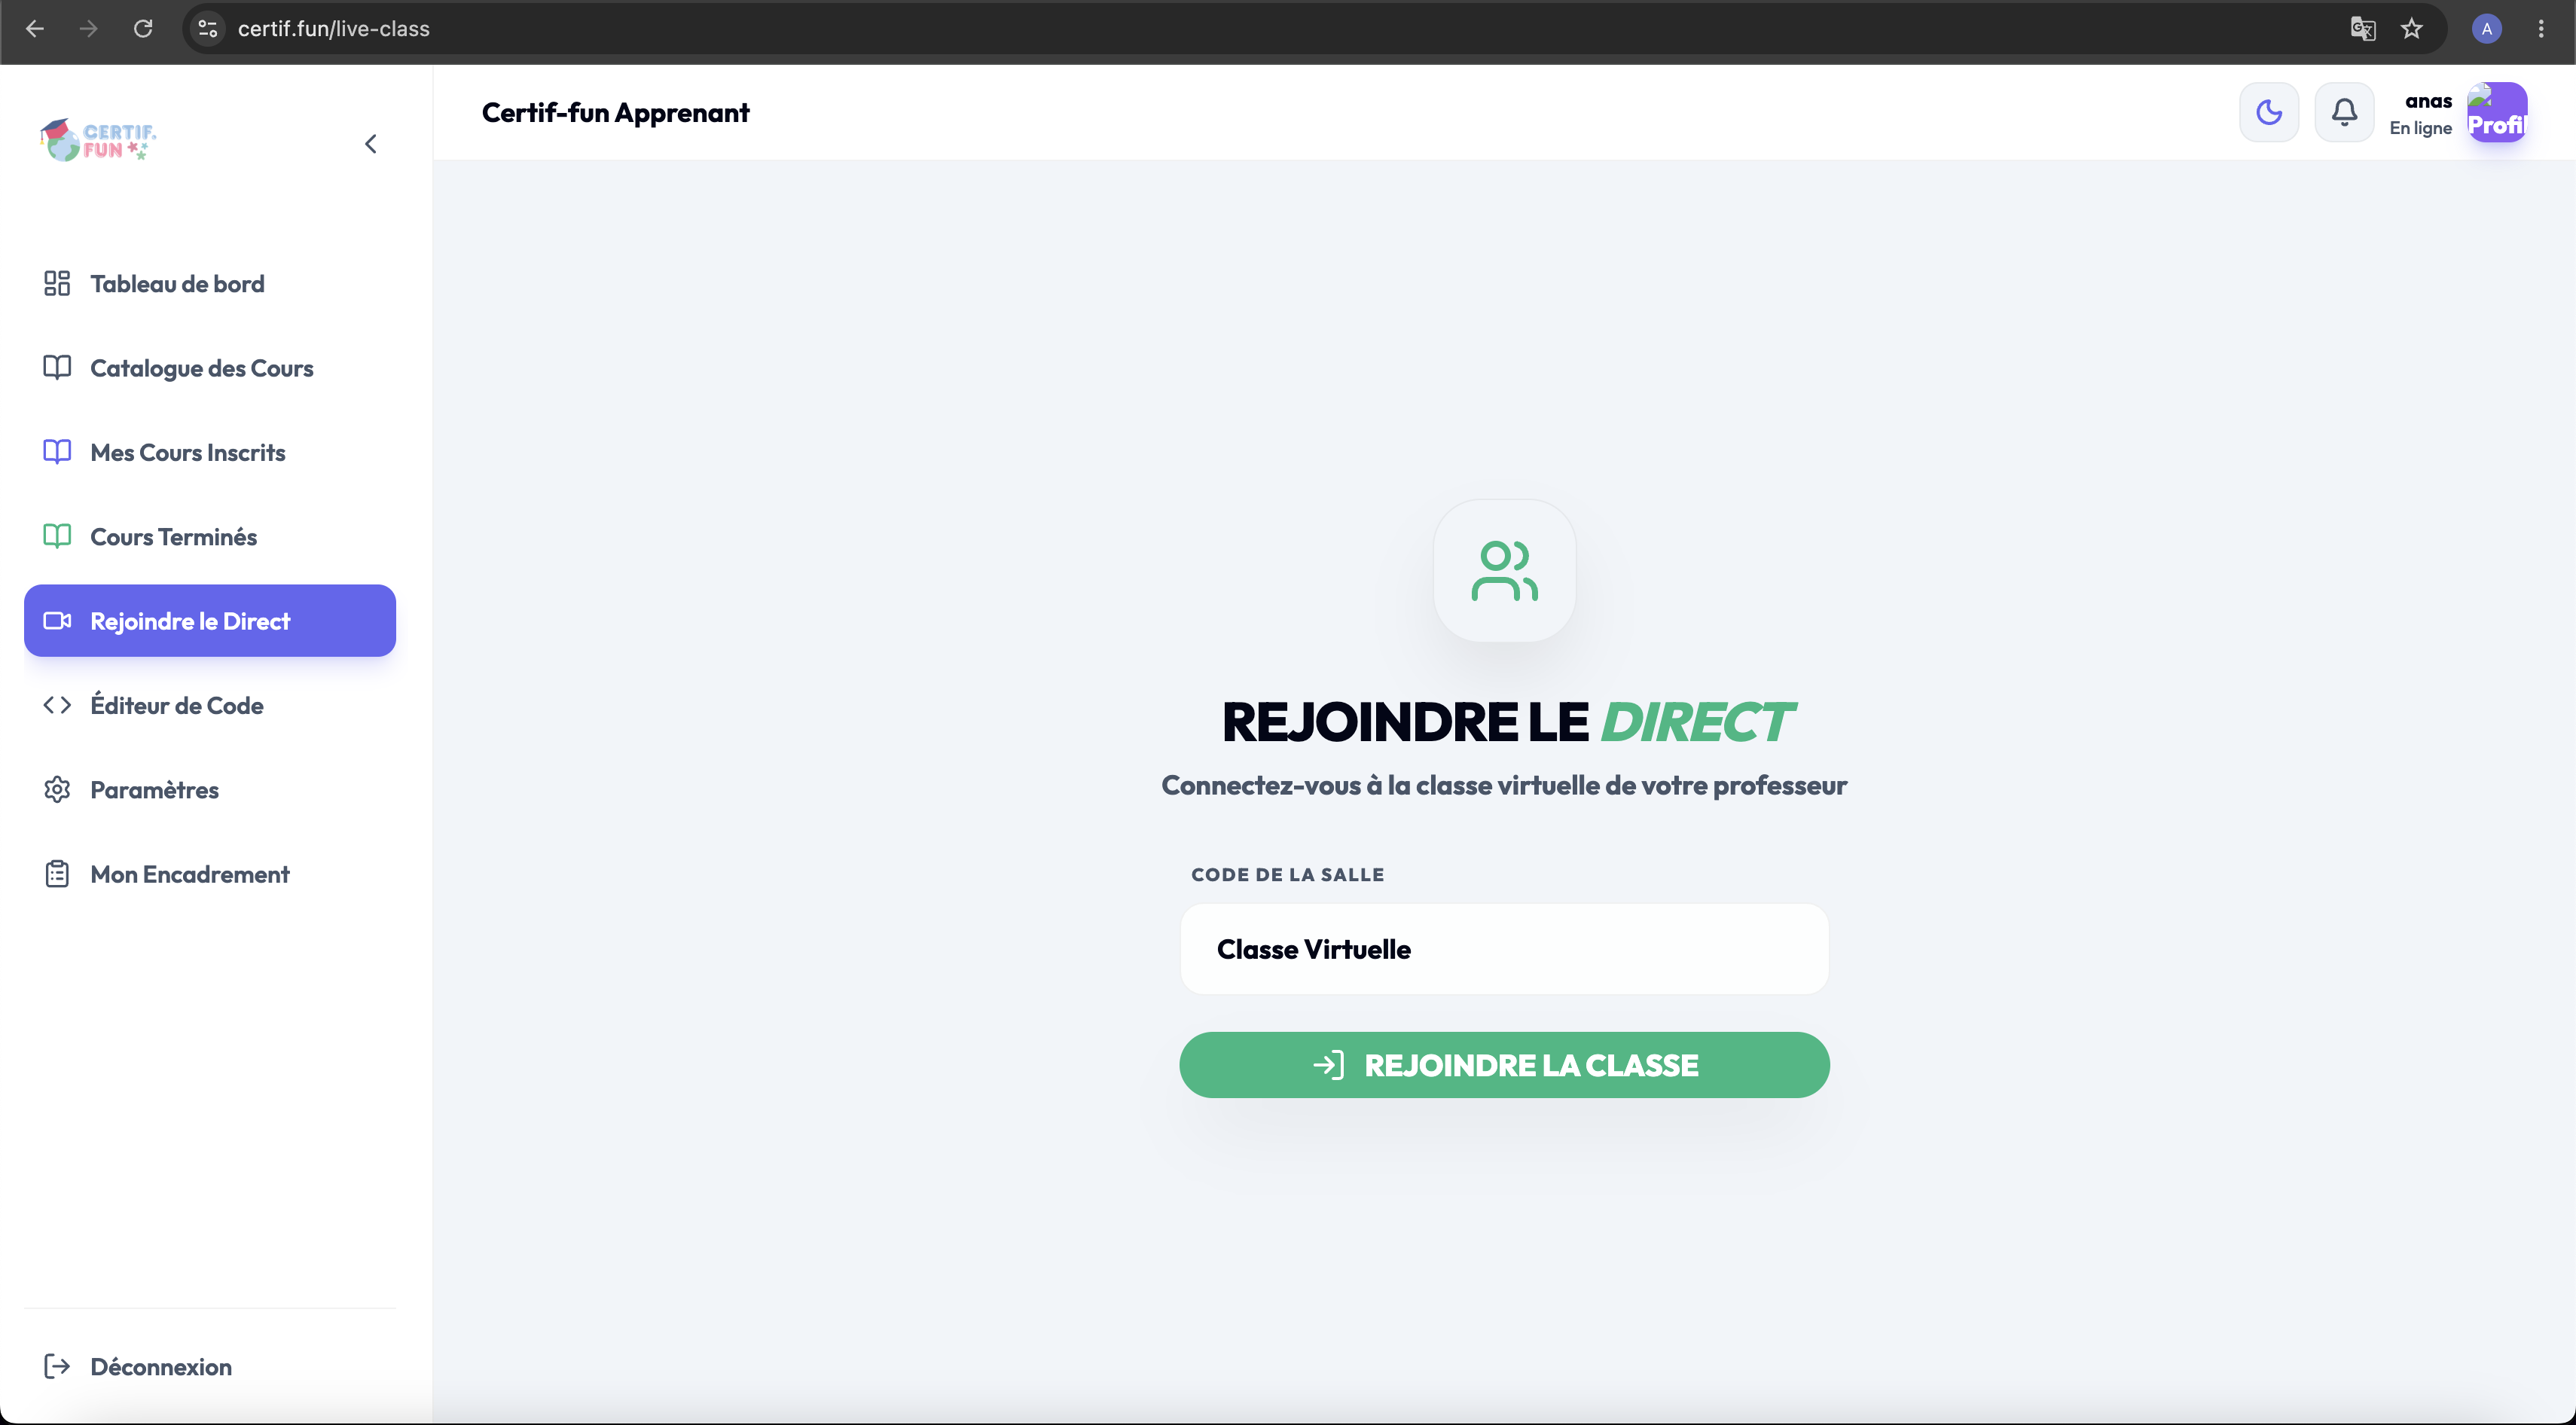
\includegraphics[width=0.98\textwidth]{figures/apprenant-4.png}
    \caption{Connexion à une session d'enseignement en direct}
    \label{fig:apprenant4}
\end{figure}

Pour les exercices pratiques en informatique, l'application propose un "Éditeur de Code" intégré (Figure~\ref{fig:apprenant5}). L'apprenant peut y rédiger et exécuter son code source de manière sécurisée (Sandbox) dans des langages comme Python, JavaScript ou Java.
\begin{figure}[H]
    \centering
    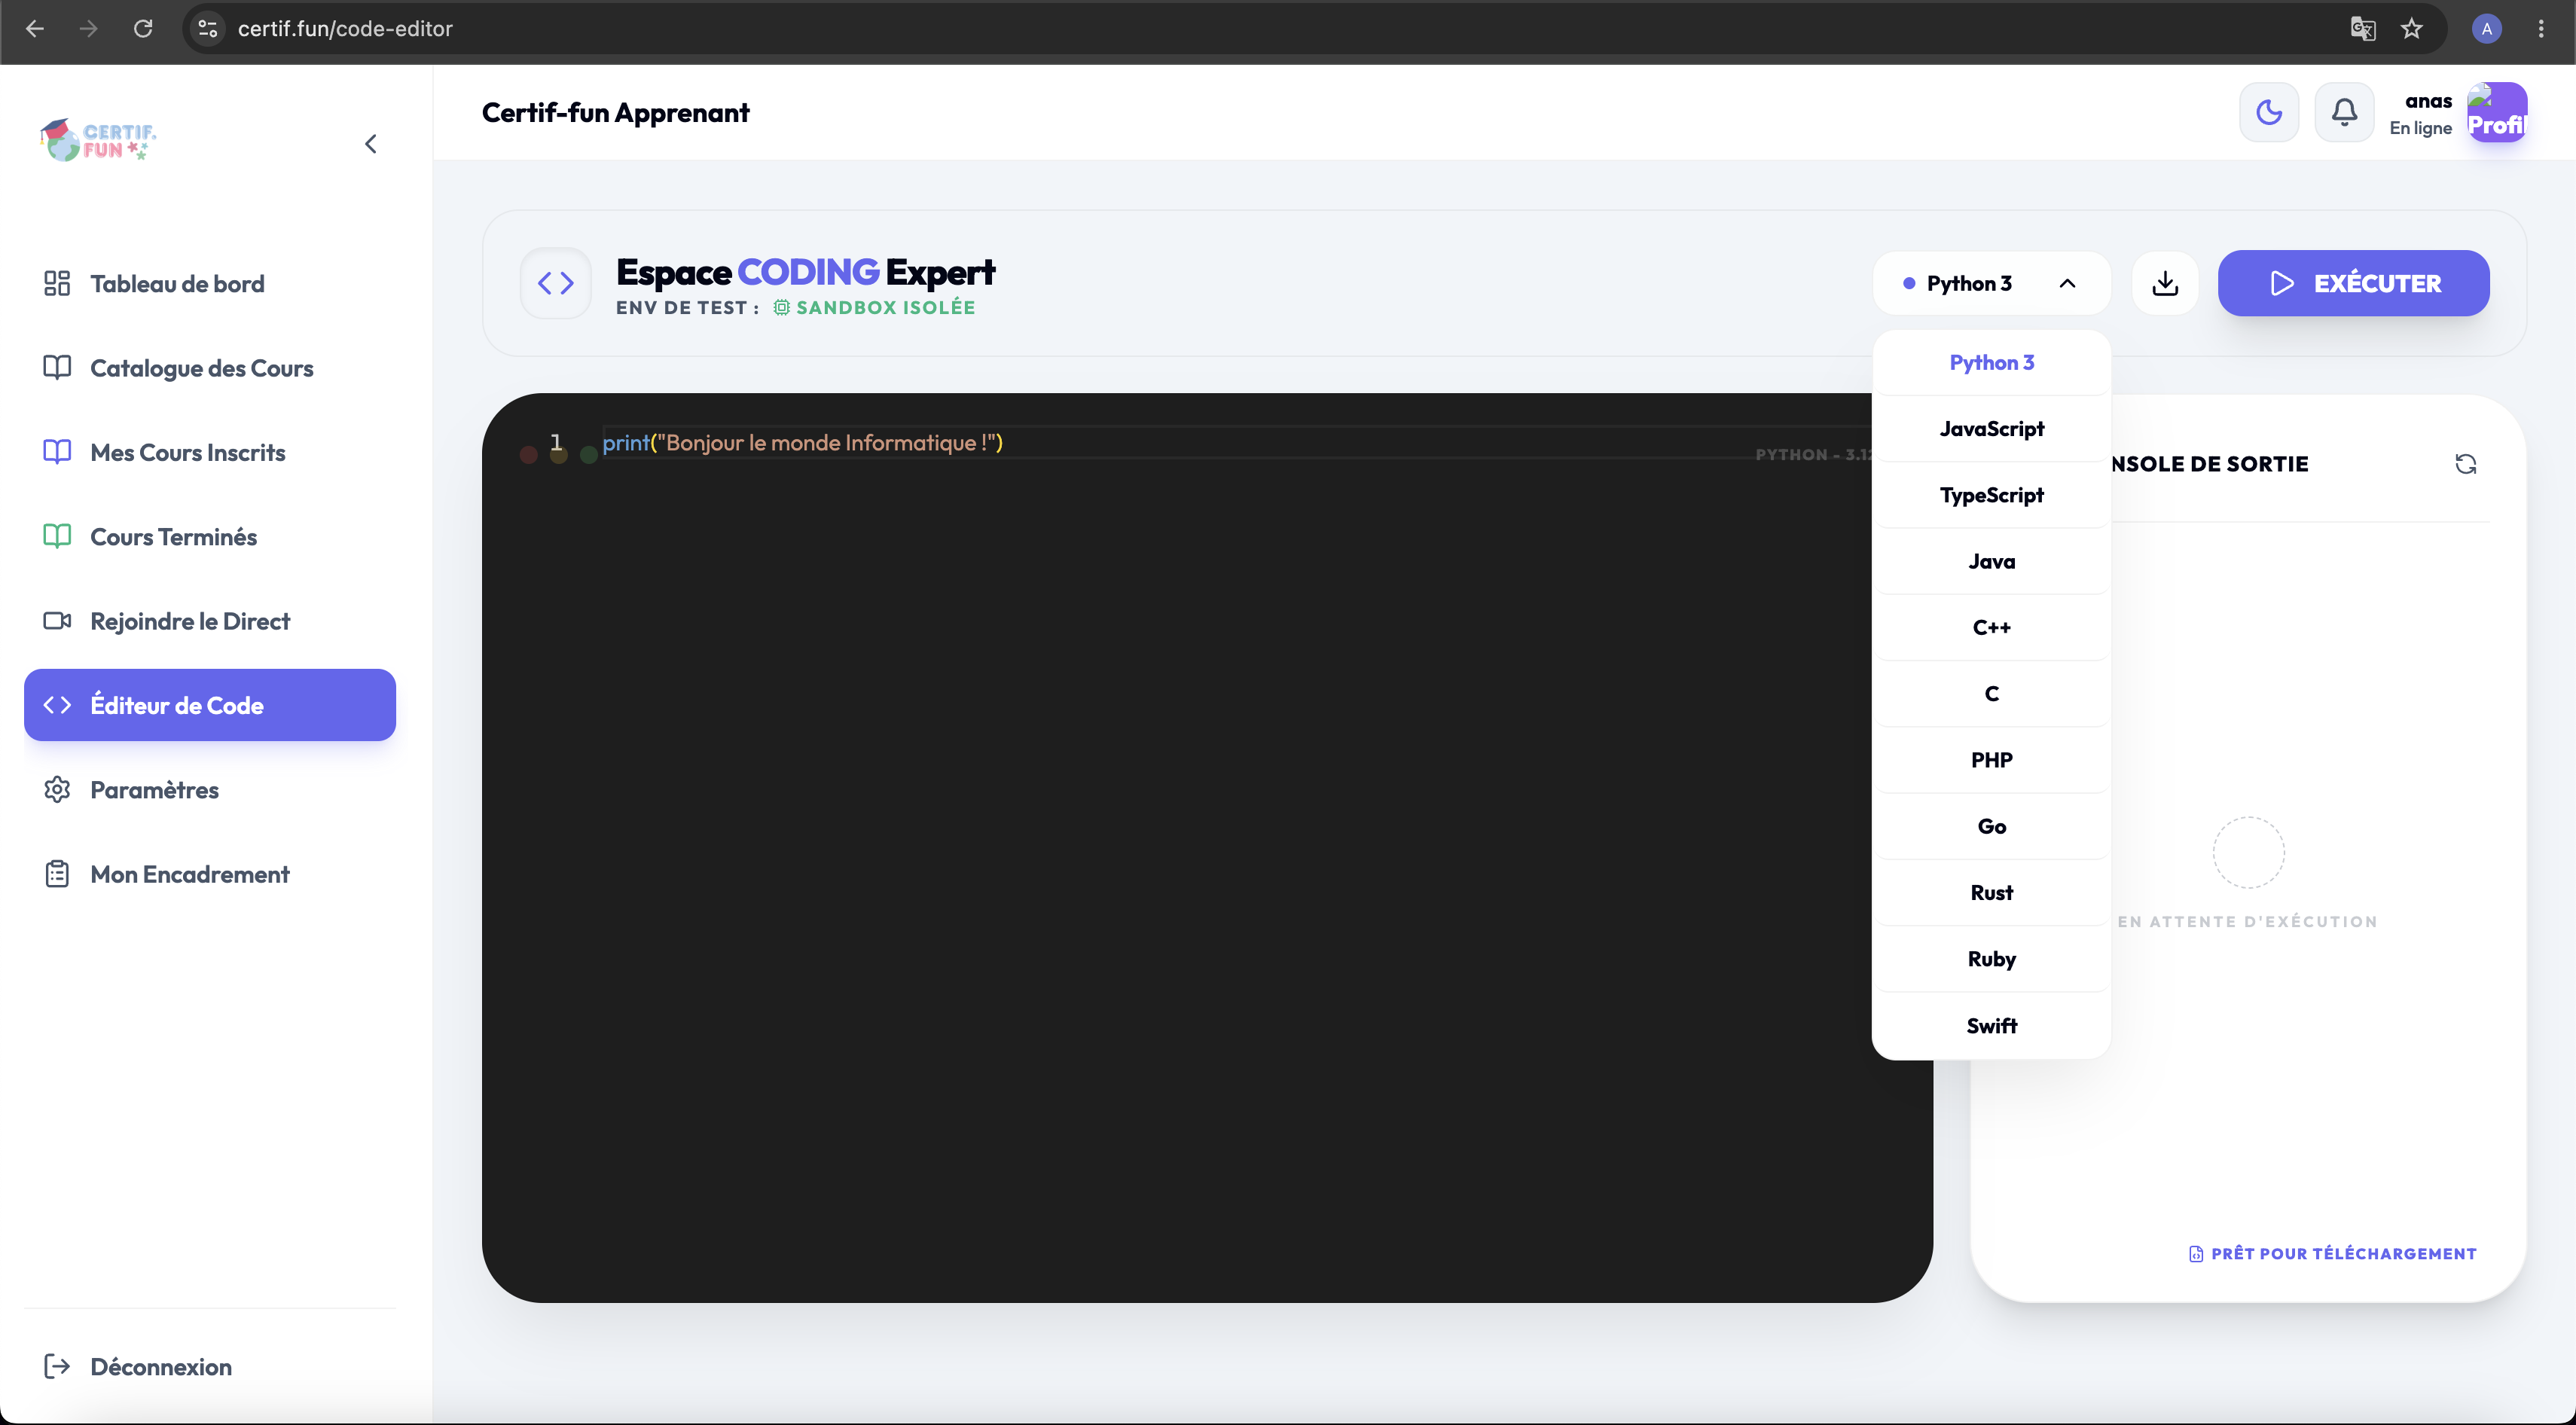
\includegraphics[width=0.98\textwidth]{figures/apprenant-5.png}
    \caption{Éditeur de code en ligne (Espace CODING Expert)}
    \label{fig:apprenant5}
\end{figure}

Enfin, le module "Mon Encadrement" (Figure~\ref{fig:apprenant6}) offre à l'étudiant un espace dédié pour la gestion de son projet de fin d'études. Il peut y visualiser sa barre de progression, ses tâches à faire et interagir avec son encadrant tout au long du projet.
\begin{figure}[H]
    \centering
    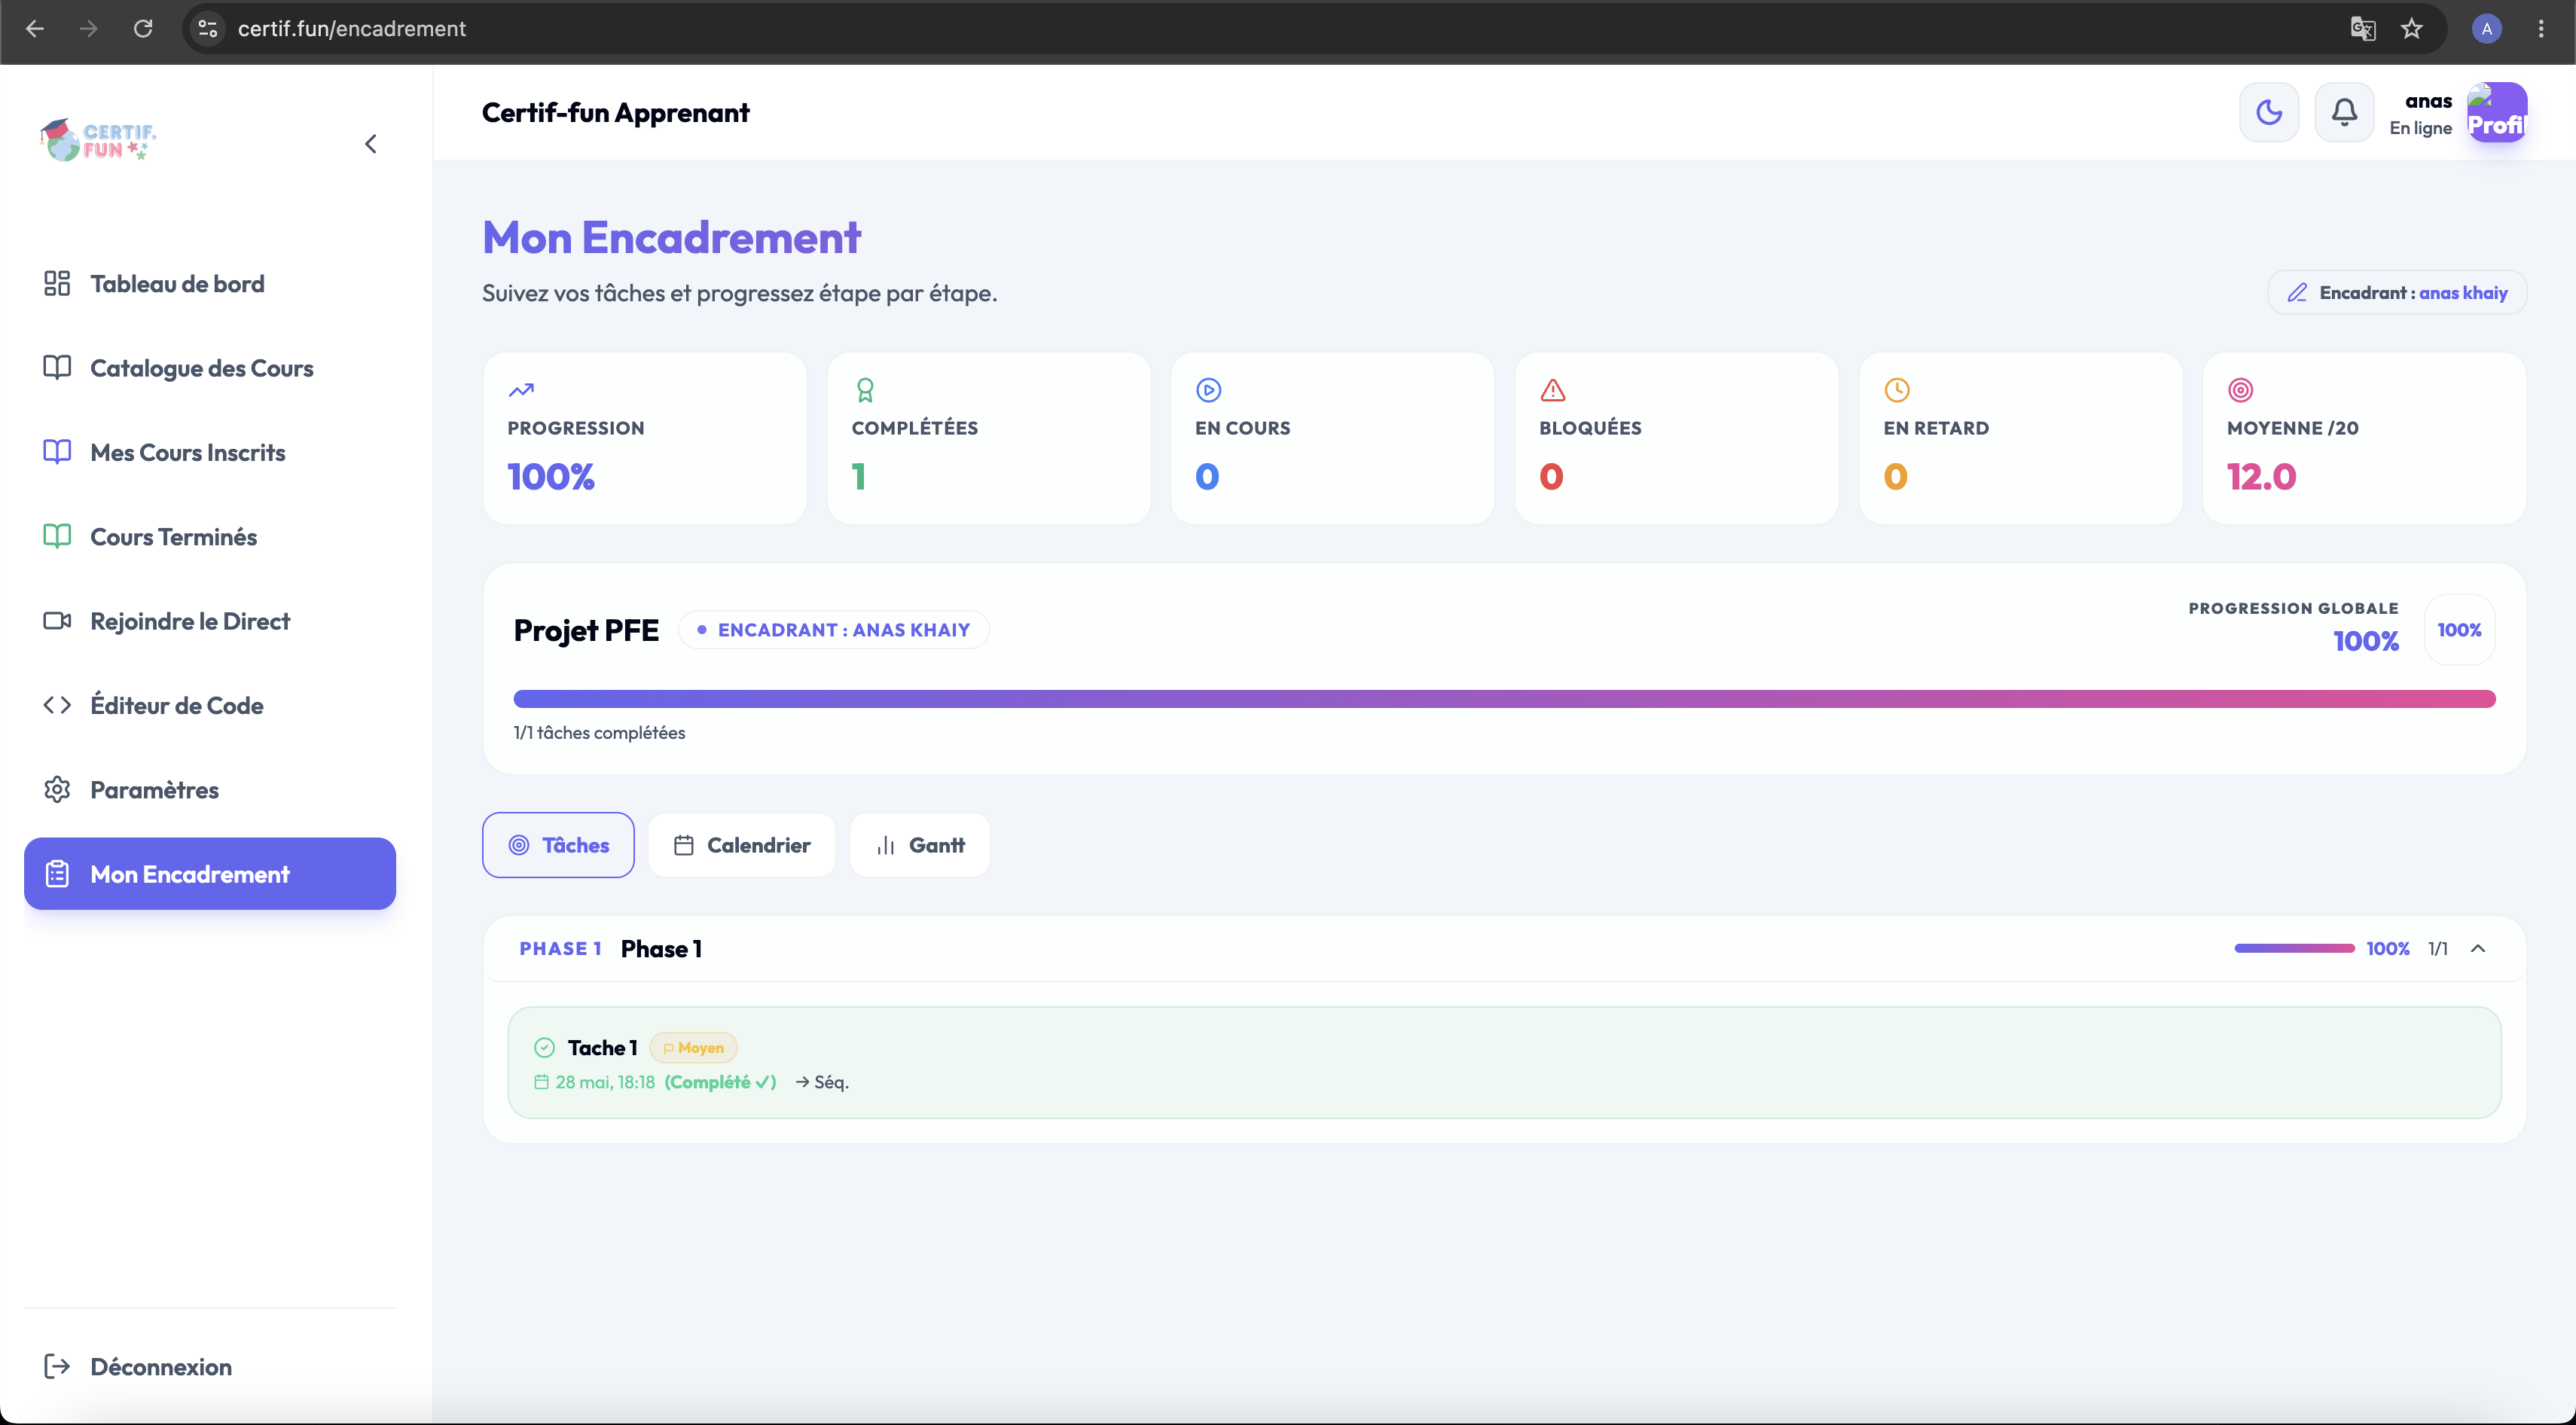
\includegraphics[width=0.98\textwidth]{figures/apprenant-6.png}
    \caption{Suivi personnalisé de l'encadrement des projets}
    \label{fig:apprenant6}
\end{figure}

L'espace d'apprentissage ou lecteur de cours (Figure~\ref{fig:apprenant7}) permet à l'étudiant de suivre le contenu pédagogique. Il dispose d'un menu de navigation latéral pour accéder aux différentes leçons et suivre sa progression. La zone principale affiche le contenu multimédia, comme des vidéos intégrées, accompagnées de textes explicatifs.
\begin{figure}[H]
    \centering
    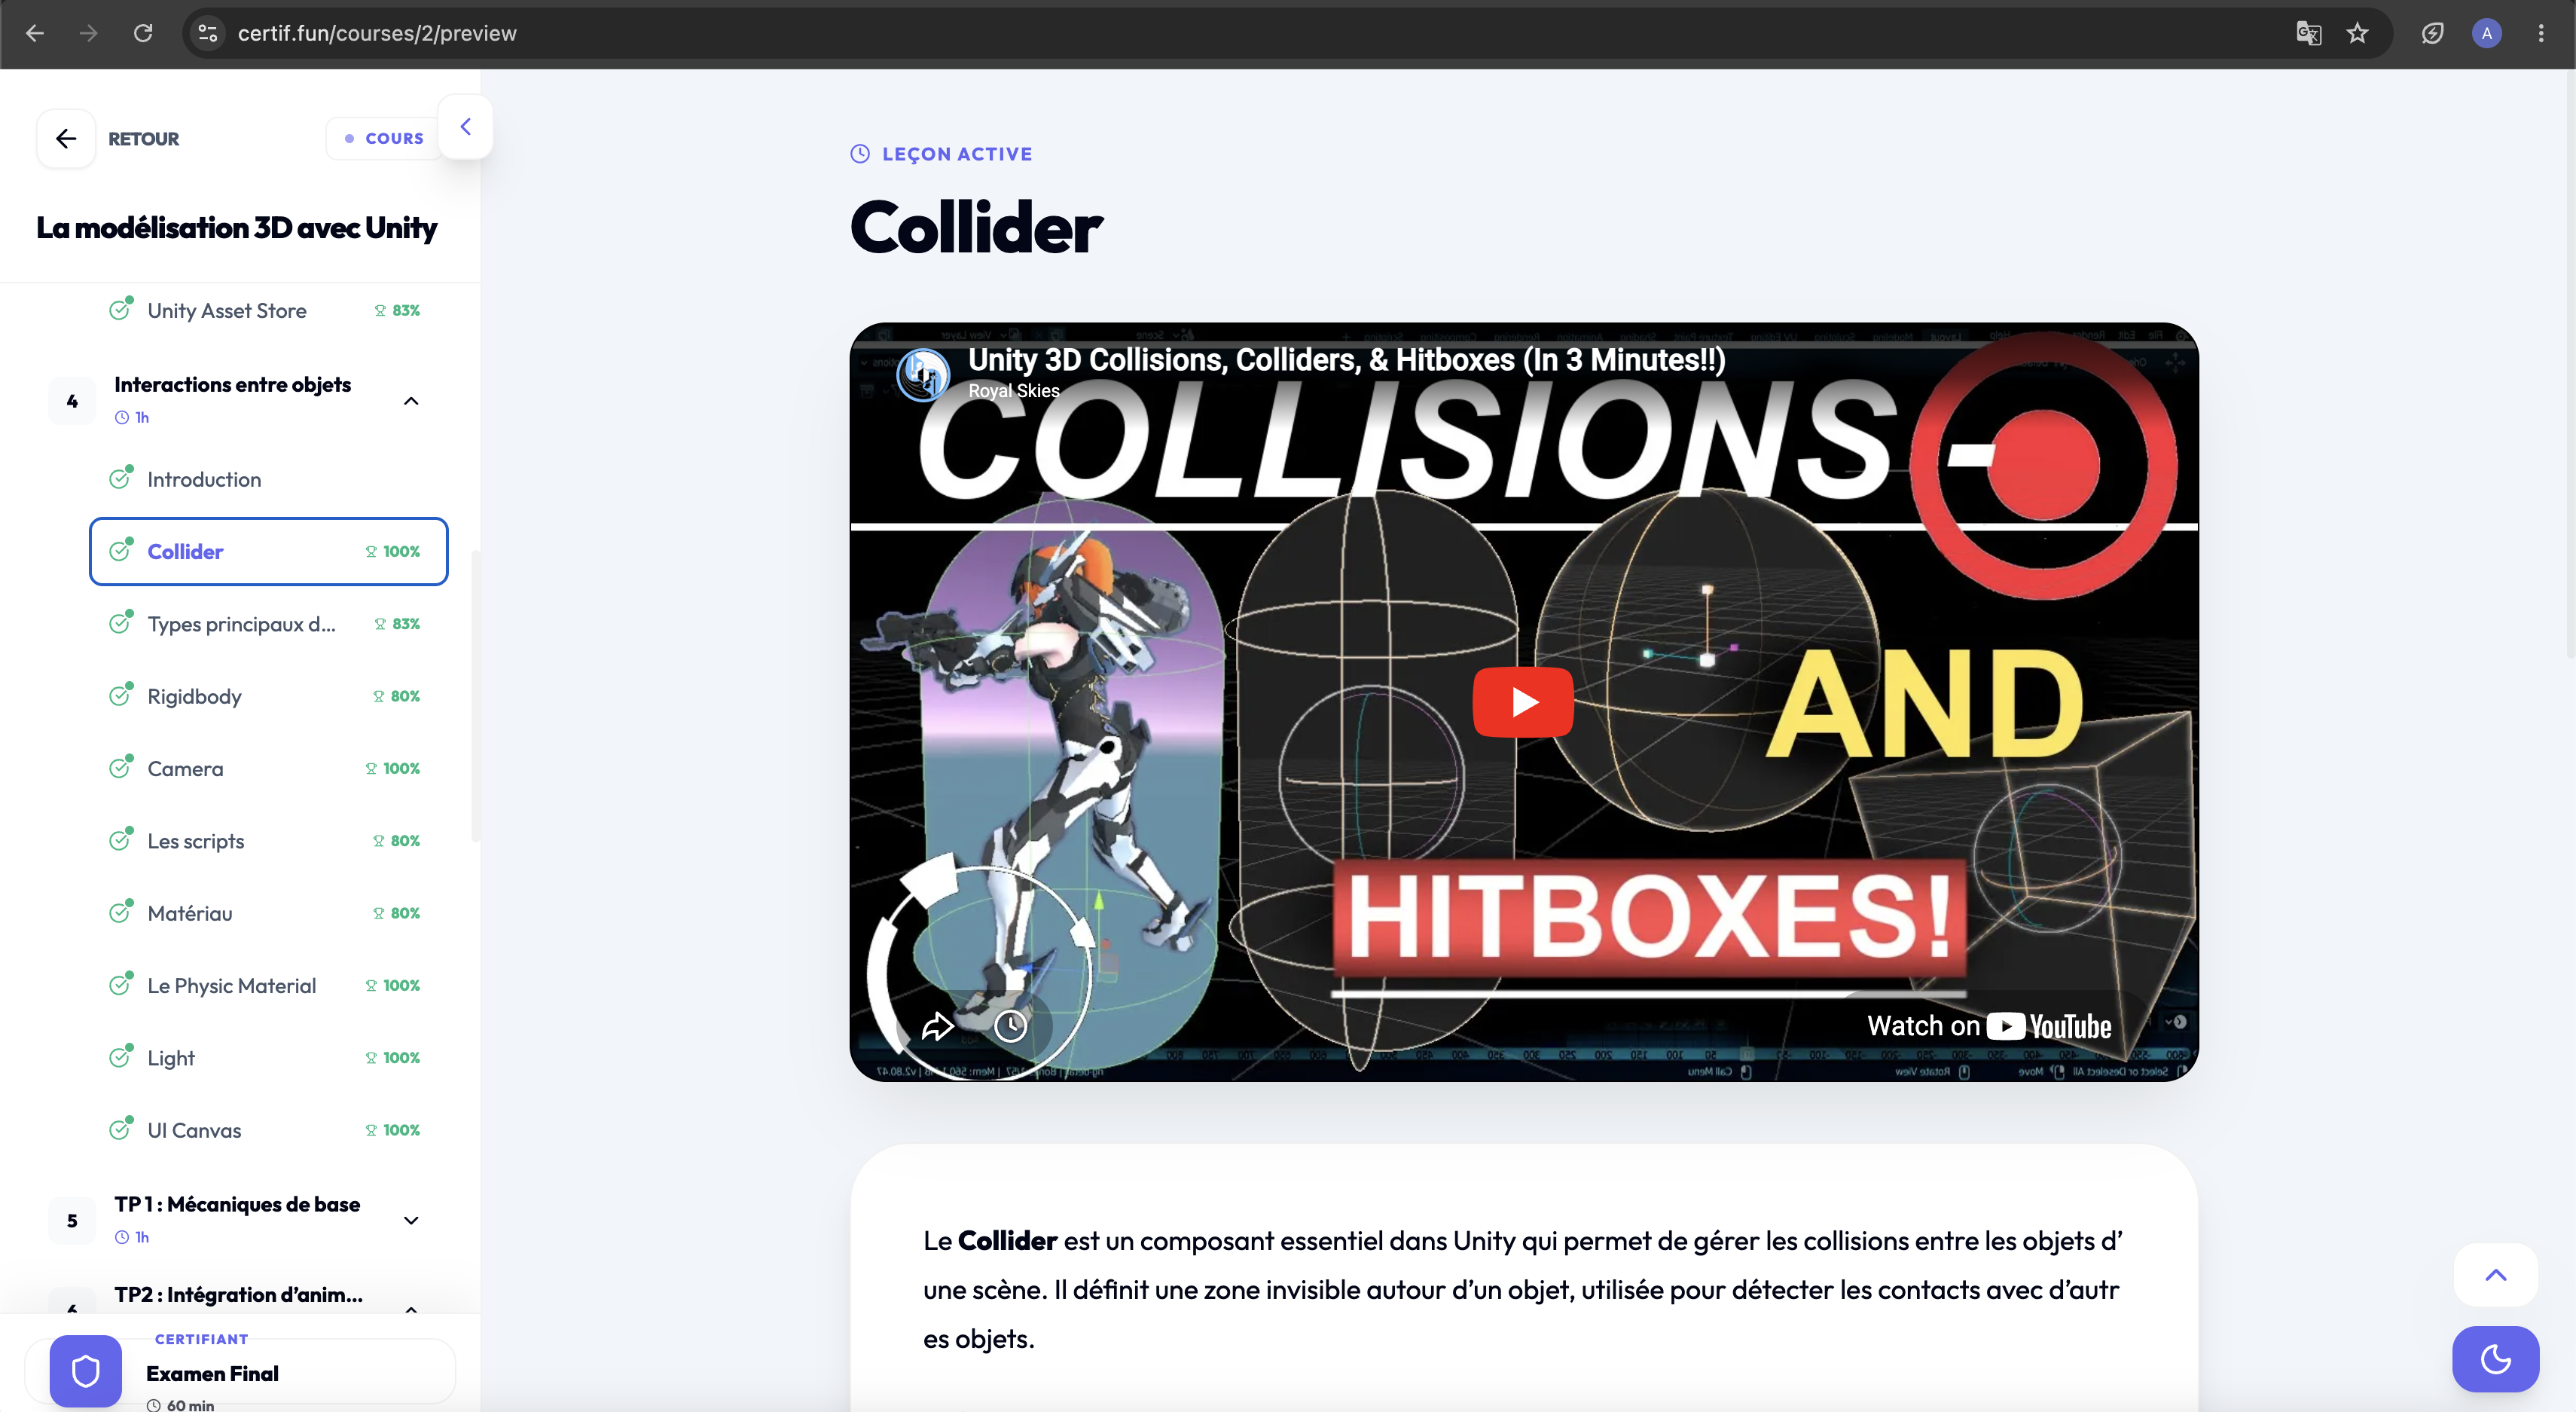
\includegraphics[width=0.98\textwidth]{figures/apprenant-7.png}
    \caption{Interface de l'espace d'apprentissage (Lecteur de cours)}
    \label{fig:apprenant7}
\end{figure}

Lors de l'évaluation, le mode examen sécurisé (Figure~\ref{fig:apprenant8}) est activé. Cette interface affiche les questions du quiz avec un chronomètre intégré. Une fenêtre de surveillance par intelligence artificielle reste active en continu, analysant le flux vidéo de l'étudiant pour assurer l'intégrité de l'épreuve. Le système surveille également le navigateur ; tout changement d'onglet ou infraction est immédiatement détecté.

\begin{figure}[H]
    \centering
    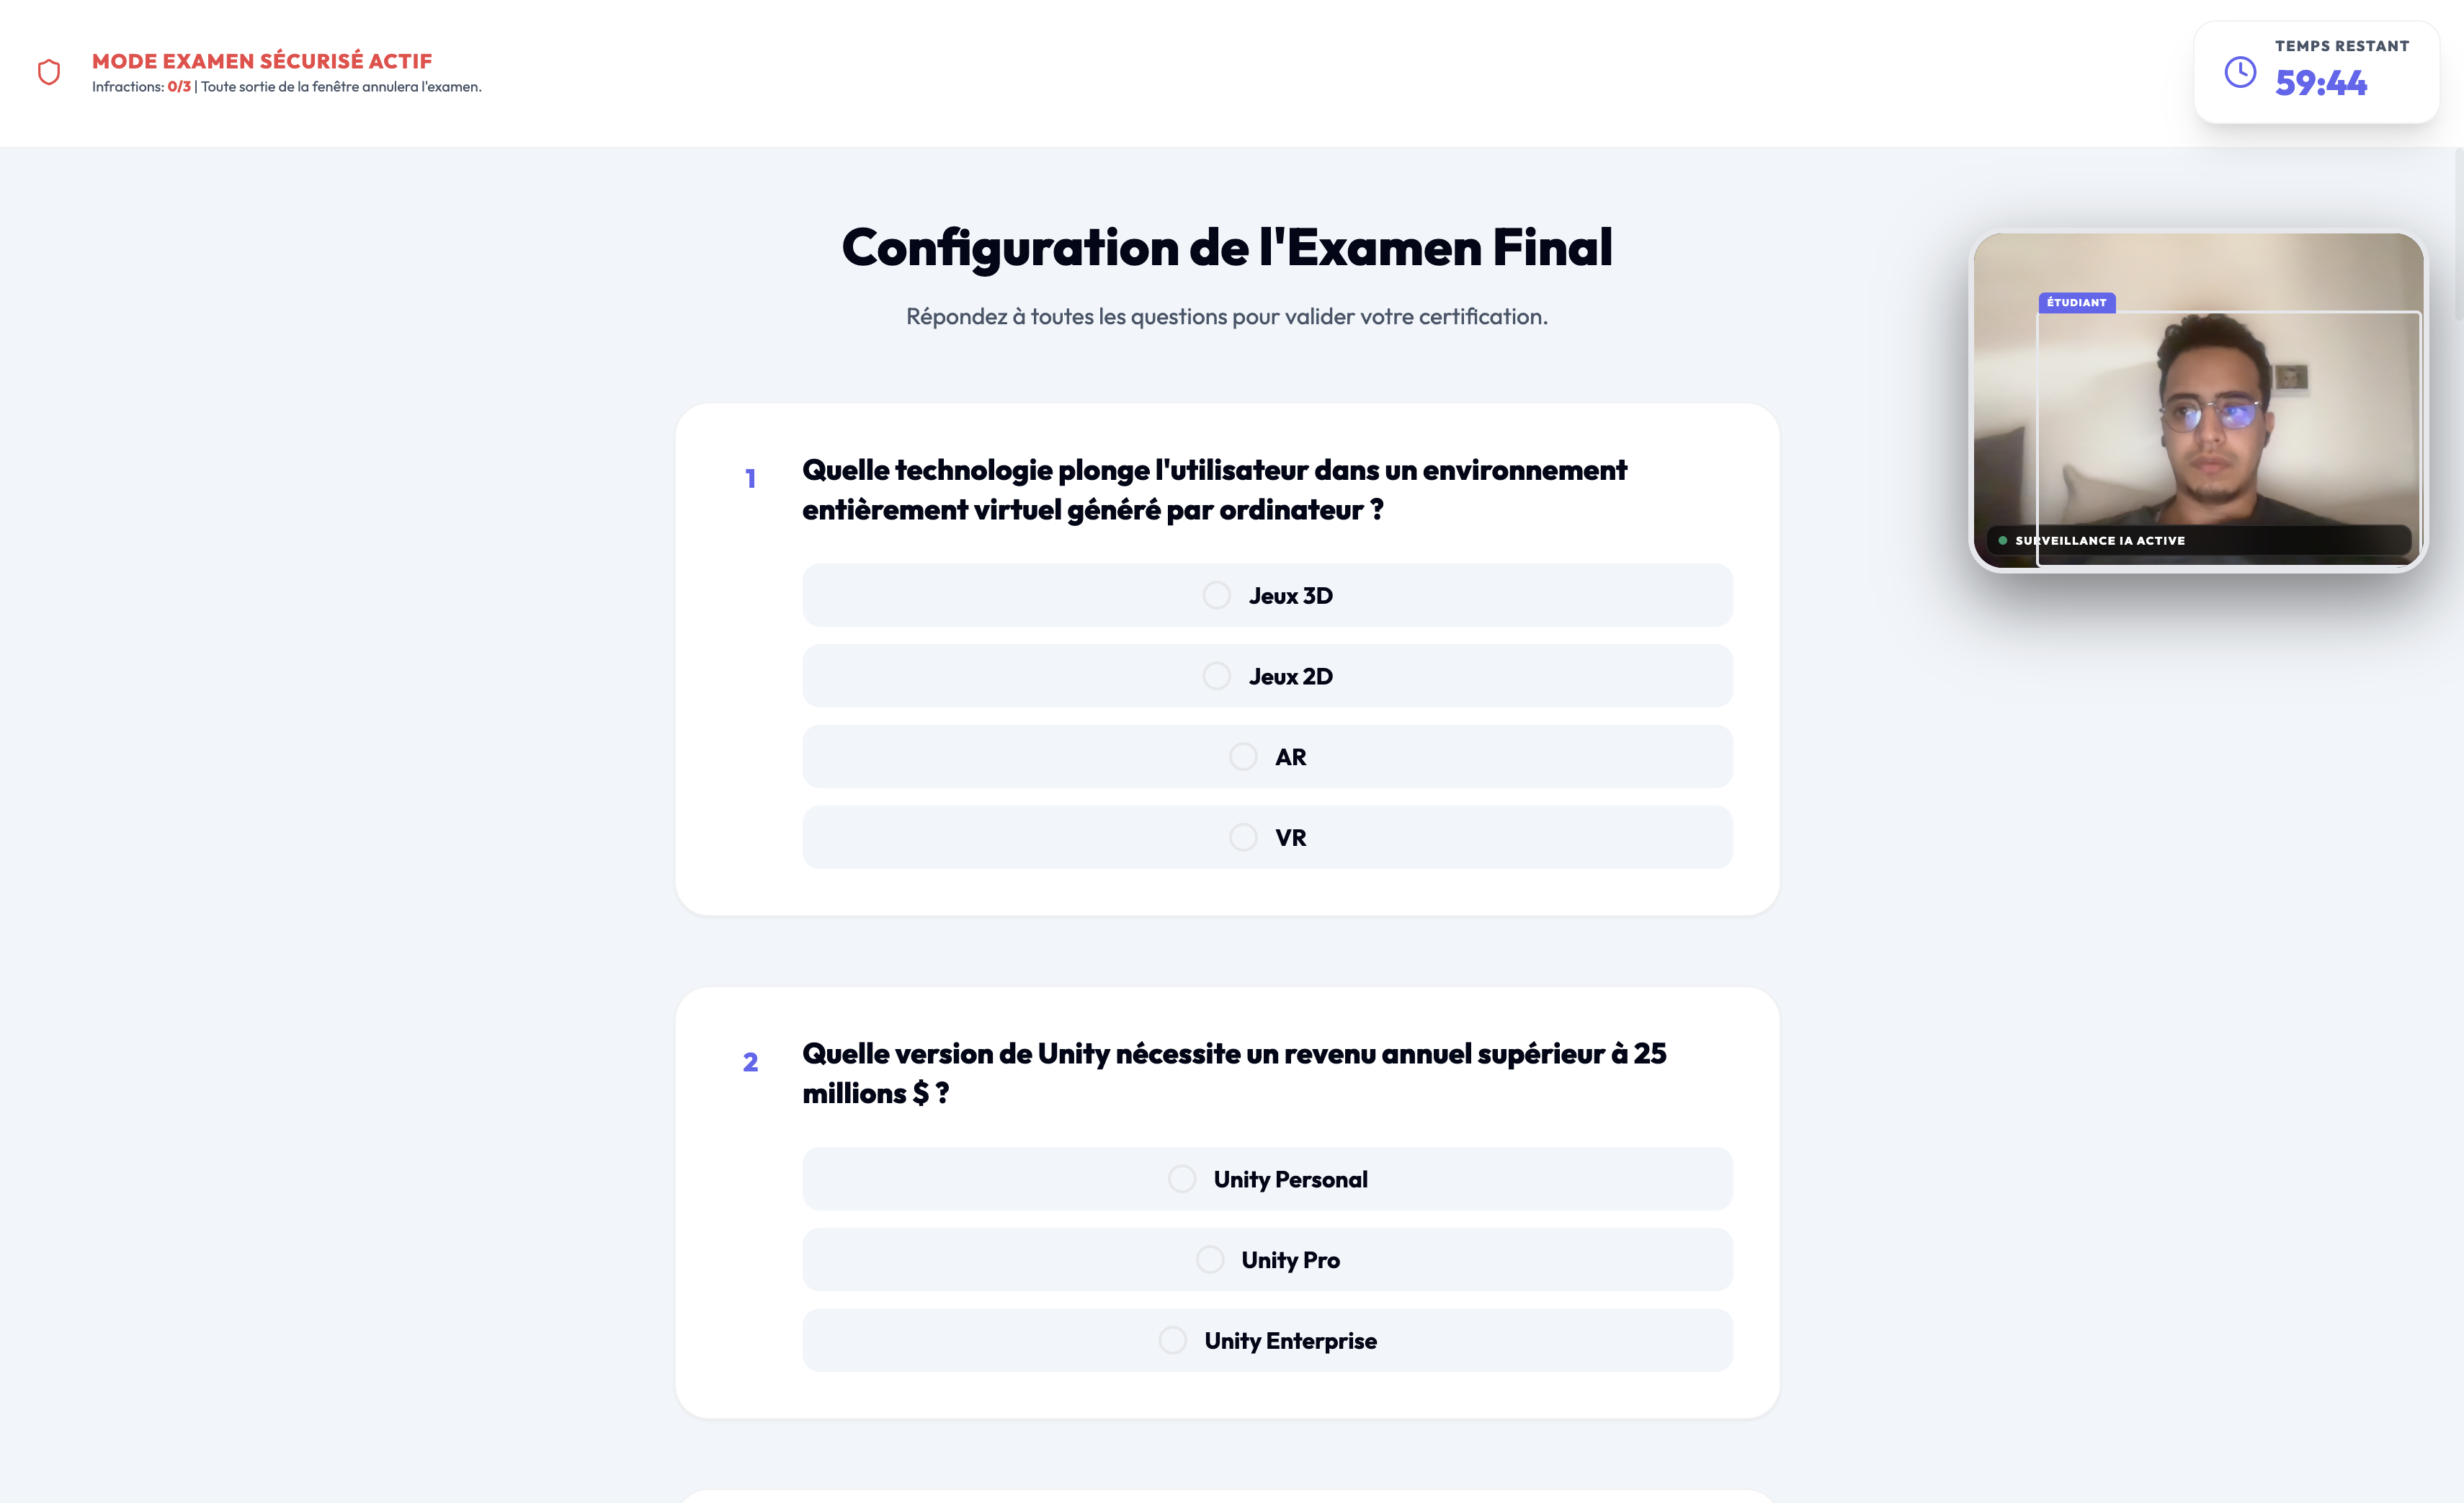
\includegraphics[width=0.98\textwidth]{figures/apprenant-8.png}
    \caption{Interface du mode examen sécurisé avec surveillance IA}
    \label{fig:apprenant8}
\end{figure}

Avant d'accéder aux questions, une étape de vérification d'identité est imposée (Figure~\ref{fig:verification_identite}). Ce module sécurisé combine le scan du code QR présent sur la carte d'étudiant pour extraire le numéro de CIN, suivi d'une comparaison biométrique faciale entre la photo de la carte et le visage réel de l'apprenant. Cette double authentification garantit que la personne présente devant la caméra est bien le candidat officiellement inscrit à la certification.

\begin{figure}[H]
    \centering
    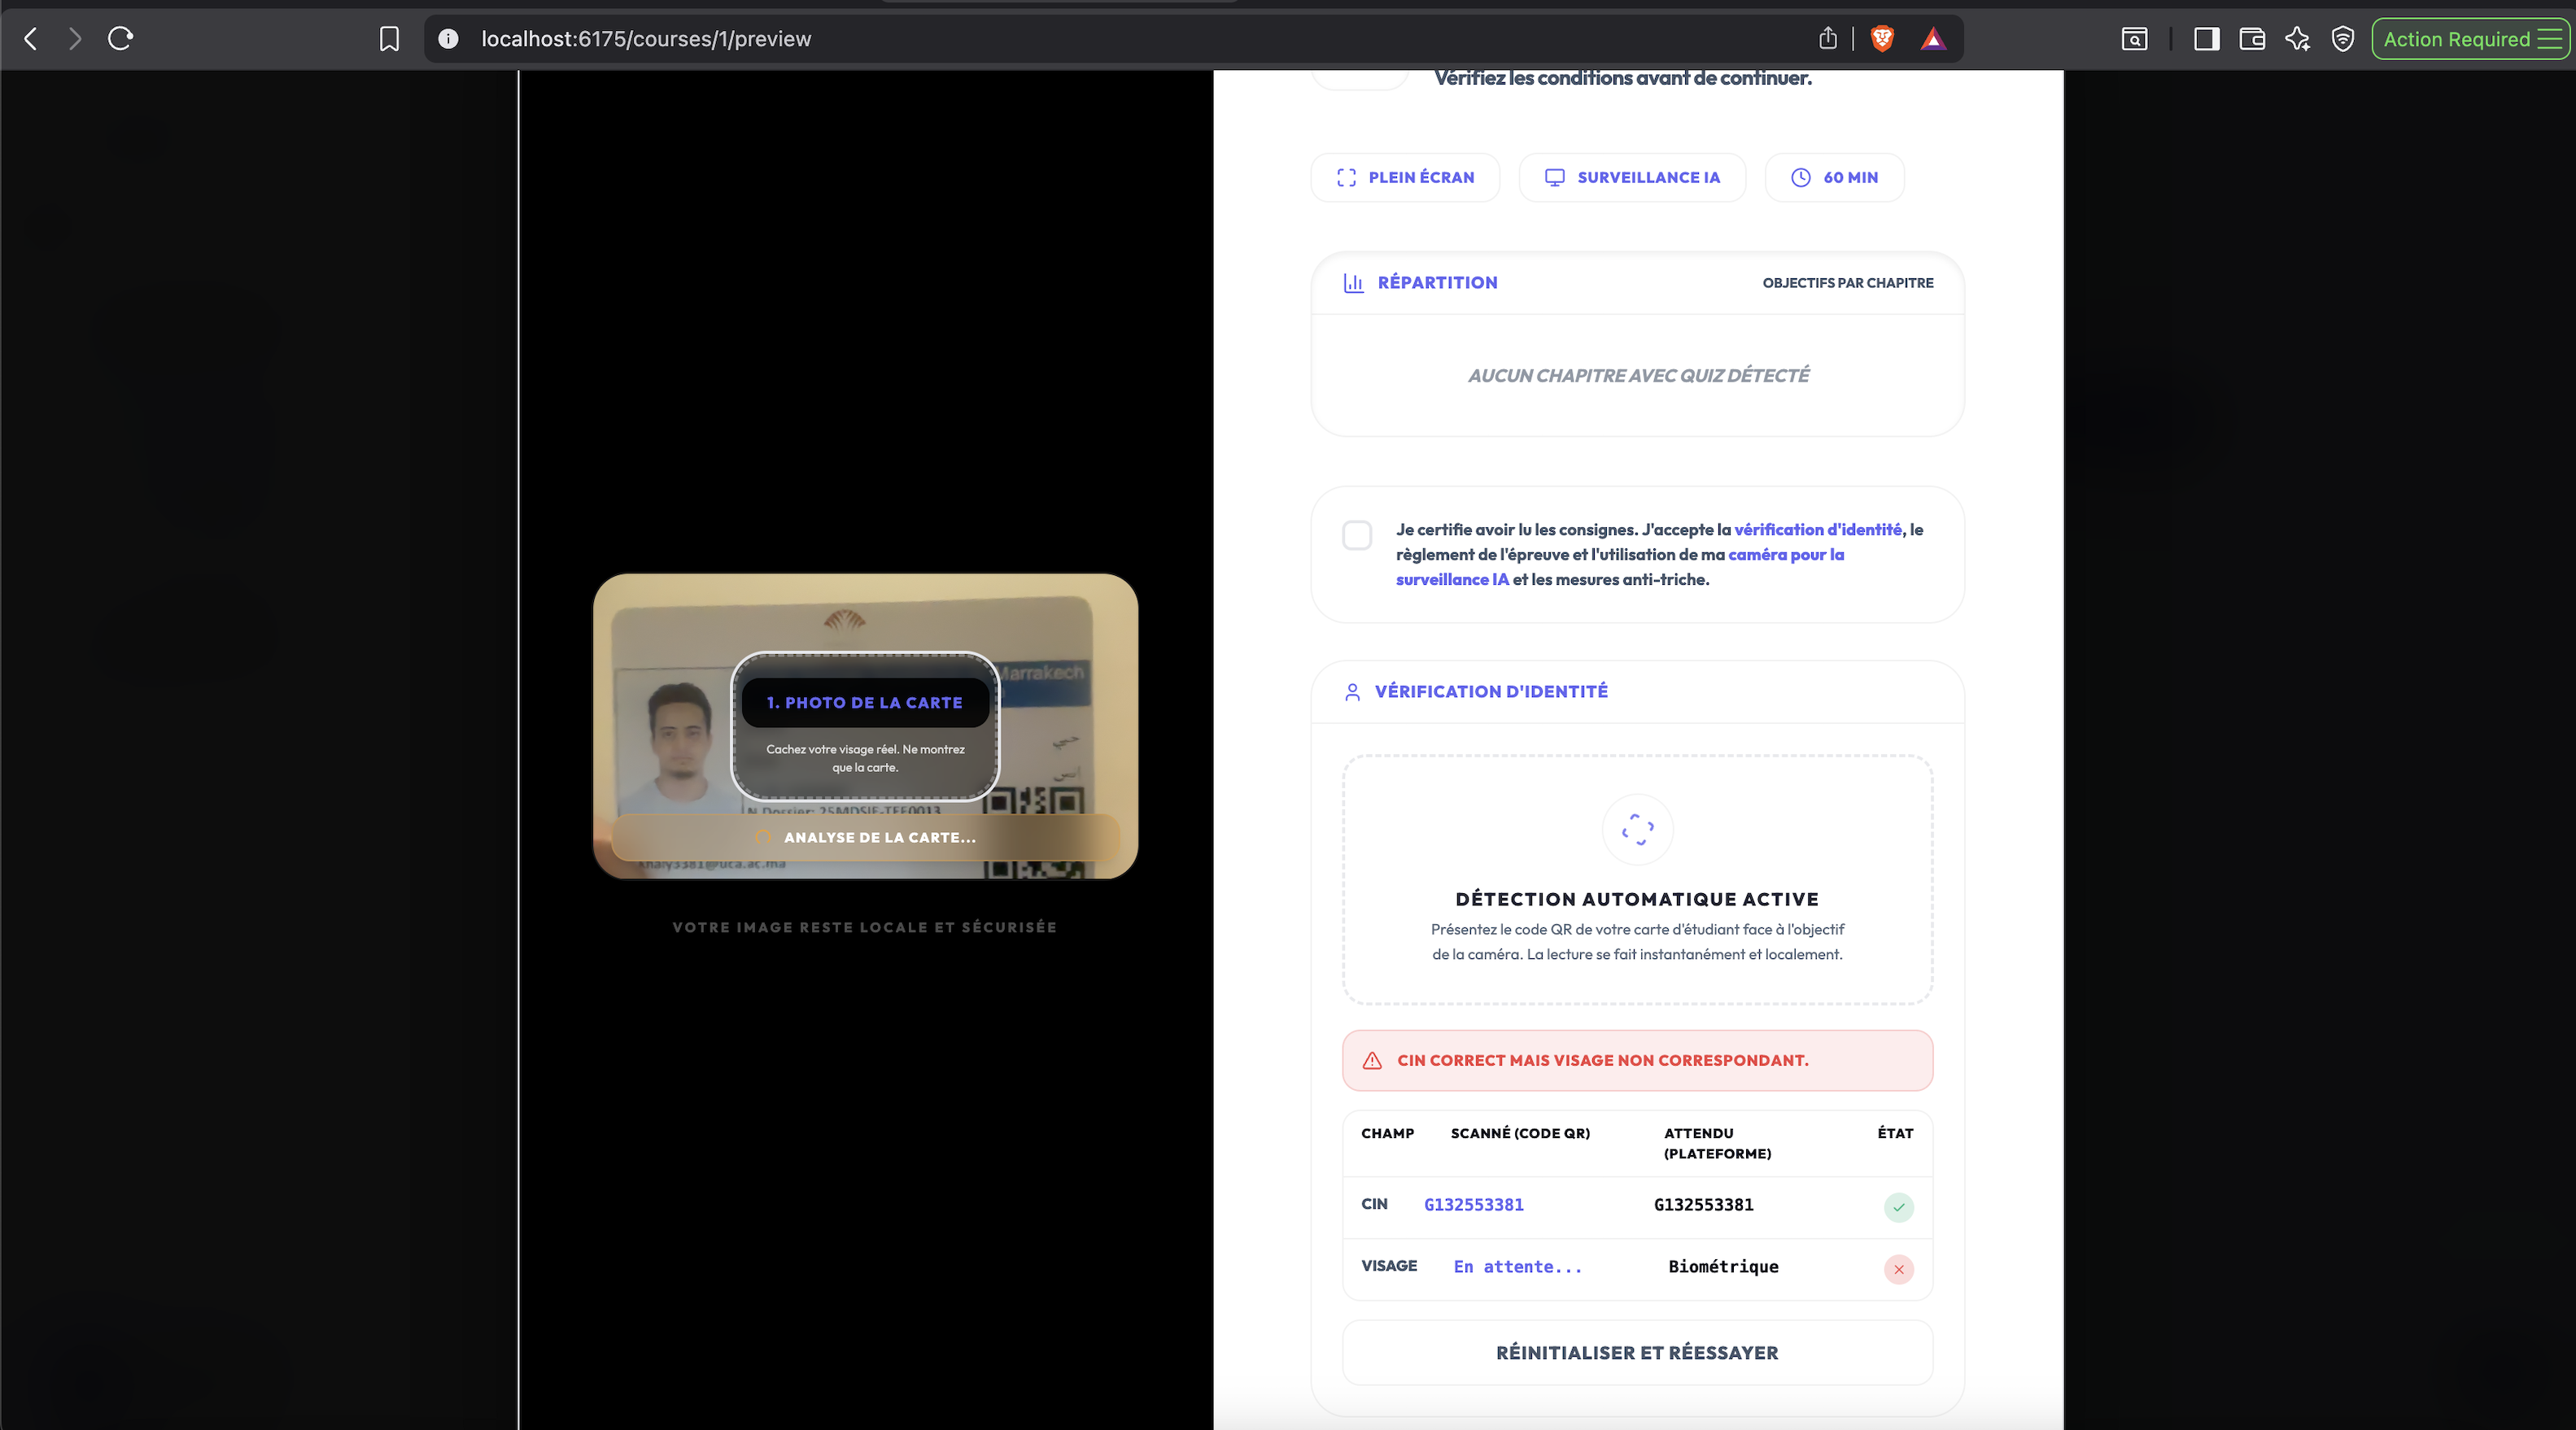
\includegraphics[width=0.98\textwidth]{figures/verification_identite.png}
    \caption{Interface de vérification d'identité (Scan QR Code et Biométrie faciale)}
    \label{fig:verification_identite}
\end{figure}


\subsection{Présentation des fonctionnalités clés}
L'implémentation de Certif-fun offre plusieurs fonctionnalités avancées pour garantir une plateforme d'apprentissage complète et sécurisée. Voici les détails techniques du fonctionnement de ces systèmes, expliqués de manière claire :

\subsubsection{Authentification et Sécurité}
La plateforme utilise un système d'authentification robuste basé sur les jetons JWT (JSON Web Token). En pratique, lorsqu'un utilisateur se connecte, le backend Spring Security vérifie ses identifiants et génère un jeton crypté. Ce jeton contient le rôle de l'utilisateur (Administrateur, Formateur ou Apprenant). À chaque nouvelle action sur la plateforme, le navigateur envoie ce jeton pour prouver l'identité de l'utilisateur, ce qui permet au système de sécuriser les données et de bloquer les accès non autorisés, sans avoir à stocker les sessions sur le serveur.

Le JSON Web Token (JWT) est un format de jeton web compact et sécurisé (codé en base64) qui permet de transmettre de manière stateless des informations (« claims ») entre deux parties. Il est souvent utilisé pour l’authentification et l’échange sécurisé de données dans les applications web \cite{mahindrakar2020jwt}.

\subsubsection{Surveillance intelligente et Détection de triche (Proctoring IA)}
Pour assurer la crédibilité des examens en ligne, le système intègre un module d'intelligence artificielle basé sur Python (FastAPI). Pendant l'examen, la caméra de l'étudiant prend des images à intervalles réguliers et les envoie au serveur :
\begin{itemize}
    \item \textbf{YOLOv8} : Ce modèle de détection d'objets analyse chaque image pour identifier l'utilisation interdite de téléphones portables ou la présence de plusieurs personnes dans la pièce \cite{sohan2025review}.
    \item \textbf{MediaPipe} : Cette technologie de suivi biométrique est utilisée pour analyser les mouvements du visage et de la tête, permettant de détecter si l'étudiant détourne son regard de l'écran pendant trop longtemps \cite{lugaresi2019mediapipe}.
    \item \textbf{Détection sonore (Web Audio API)} : Le système analyse le flux audio du microphone pour identifier les bruits continus ou la parole, déclenchant une alerte automatique après 5 secondes de perturbation sonore suspecte.
    \item \textbf{Surveillance du navigateur} : Le système détecte via JavaScript si l'étudiant quitte le mode plein écran ou ouvre un nouvel onglet.
\end{itemize}
Toute infraction détectée incrémente un compteur. Si le seuil de tolérance est dépassé, l'examen est automatiquement annulé.

\subsubsection{Génération automatique de Quiz et de Contenu}
Pour faciliter le travail des formateurs, Certif-fun intègre un générateur de quiz propulsé par l'intelligence artificielle générative (Mistral 7B via Ollama). Le système fonctionne ainsi : le formateur insère le texte de son cours, puis le backend envoie un \textit{prompt} (une instruction stricte) à l'IA locale \cite{novais2025using}. L'IA analyse le texte et retourne un format de données structuré (JSON) contenant des questions à choix multiples pertinentes, ainsi que les bonnes options de réponse.

\subsubsection{Éditeur de Code en ligne interactif}
Pour les formations en informatique, Certif-fun propose l'espace "Coding Expert". Le fonctionnement de cet éditeur repose sur l'envoi du code écrit par l'étudiant dans son navigateur vers le serveur backend. Le serveur compile et exécute ce code (par exemple du Python ou du Java) dans un environnement isolé, puis renvoie instantanément le résultat de l'exécution ou les éventuelles erreurs à l'écran de l'étudiant. Cela permet une pratique immédiate sans nécessiter d'installation de logiciels.

\subsubsection{Visioconférence et Classes Virtuelles}
Les sessions vidéo en direct sont rendues possibles par la technologie \textbf{LiveKit} \cite{livekit_docs}. Le backend Spring Boot est chargé de générer des "Tokens" d'accès temporaires. Le navigateur de l'étudiant utilise ce Token pour se connecter à un serveur de streaming LiveKit (via le protocole WebRTC \cite{romano2012webrtc}). Cela permet d'établir une communication vidéo et audio fluide, à très faible latence, directement entre le formateur et les apprenants, avec la possibilité de partager son écran.

\subsubsection{Encadrement des Projets}
Le module d'encadrement des projets est géré par une structure de données qui relie le formateur, l'étudiant et le projet. Le système s'apparente à un tableau Kanban (À faire, En cours, Terminé). Chaque fois qu'une tâche est validée, le backend recalcule le pourcentage d'avancement du projet et met à jour en temps réel la barre de progression sur le tableau de bord partagé, assurant ainsi un suivi transparent des dates limites.

%%%%%%%%%%%%%%%%%%%%%%%%%%%%%%%%%%%%%%%%%%%%%%%%%%%%%%%%%%%
\section{Stratégie de tests et validation}
%%%%%%%%%%%%%%%%%%%%%%%%%%%%%%%%%%%%%%%%%%%%%%%%%%%%%%%%%%%
La fiabilité de Certif-fun a été éprouvée par une pyramide de tests rigoureuse visant à garantir la qualité et la robustesse du système. Cette approche structurée permet de détecter au plus tôt les régressions, de valider la logique métier de manière isolée et d'assurer une intégration fiable de l'ensemble des microservices et des modules d'intelligence artificielle.

\subsection{Tests Unitaires}
L'un des défis majeurs dans le test des architectures microservices et des applications basées sur l'intelligence artificielle est la dépendance vis-à-vis des composants externes (tels que la base de données PostgreSQL, le serveur SMTP d'envoi de courriels, ou le chargement lourd en mémoire de modèles Deep Learning comme YOLOv8).

Pour surmonter ces contraintes, nous avons adopté une philosophie de \textbf{tests unitaires isolés} reposant sur le \textbf{bouchonnage (mocking)}. En isolant chaque composant métier, nous garantissons une exécution rapide, déterministe et une couverture ciblée des cas d'erreur.

\subsubsection{Détail des tests unitaires Java (JUnit 5 \& Mockito)}
Pour les trois microservices Spring Boot (Backend-Admin, Backend-Apprenant et Backend-Formateur), nous avons développé une suite exhaustive comprenant plus d'une centaine de tests unitaires \cite{kleuker2019junit5}.

\paragraph{1. Tests d'intégration de fichiers volumineux (\texttt{ExcelImportServiceTest}) :}
Au sein du \texttt{Backend-Admin}, l'importation massive d'étudiants se fait via des fichiers XLSX. Nous avons implémenté des tests pour valider la structure des fichiers et la gestion des doublons.

\paragraph{2. Tests de logique transactionnelle (\texttt{EnrollmentServiceTest}) :}
Dans le \texttt{Backend-Apprenant}, des scénarios vérifient le blocage de la concurrence (Race Conditions) et la validation des prérequis métier pour l'accès aux modules.

\paragraph{3. Tests de résilience face aux API externes (\texttt{QuizAIServiceTest}) :}
Pour le \texttt{Backend-Formateur}, nous avons bouchonné le \texttt{RestTemplate} pour simuler des timeouts et valider le mécanisme de secours (fallback) lors de la génération de quiz par IA.

\subsubsection{Détail des tests unitaires Python (pytest \& FastAPI)}
Pour le module d'intelligence artificielle (\texttt{AI-Detection-Service}), la suite de tests s'appuie sur \texttt{pytest} \cite{pytest_docs} et mocke les modèles YOLOv8 et MediaPipe pour valider les scénarios de triche et la robustesse des données entrantes.

\subsubsection{Résultats d'exécution des tests unitaires}
La figure~\ref{fig:test_unitaire} présente une capture d'écran réelle de l'exécution de la suite de tests unitaires, confirmant un succès de 100\%.

\begin{figure}[H]
    \centering
    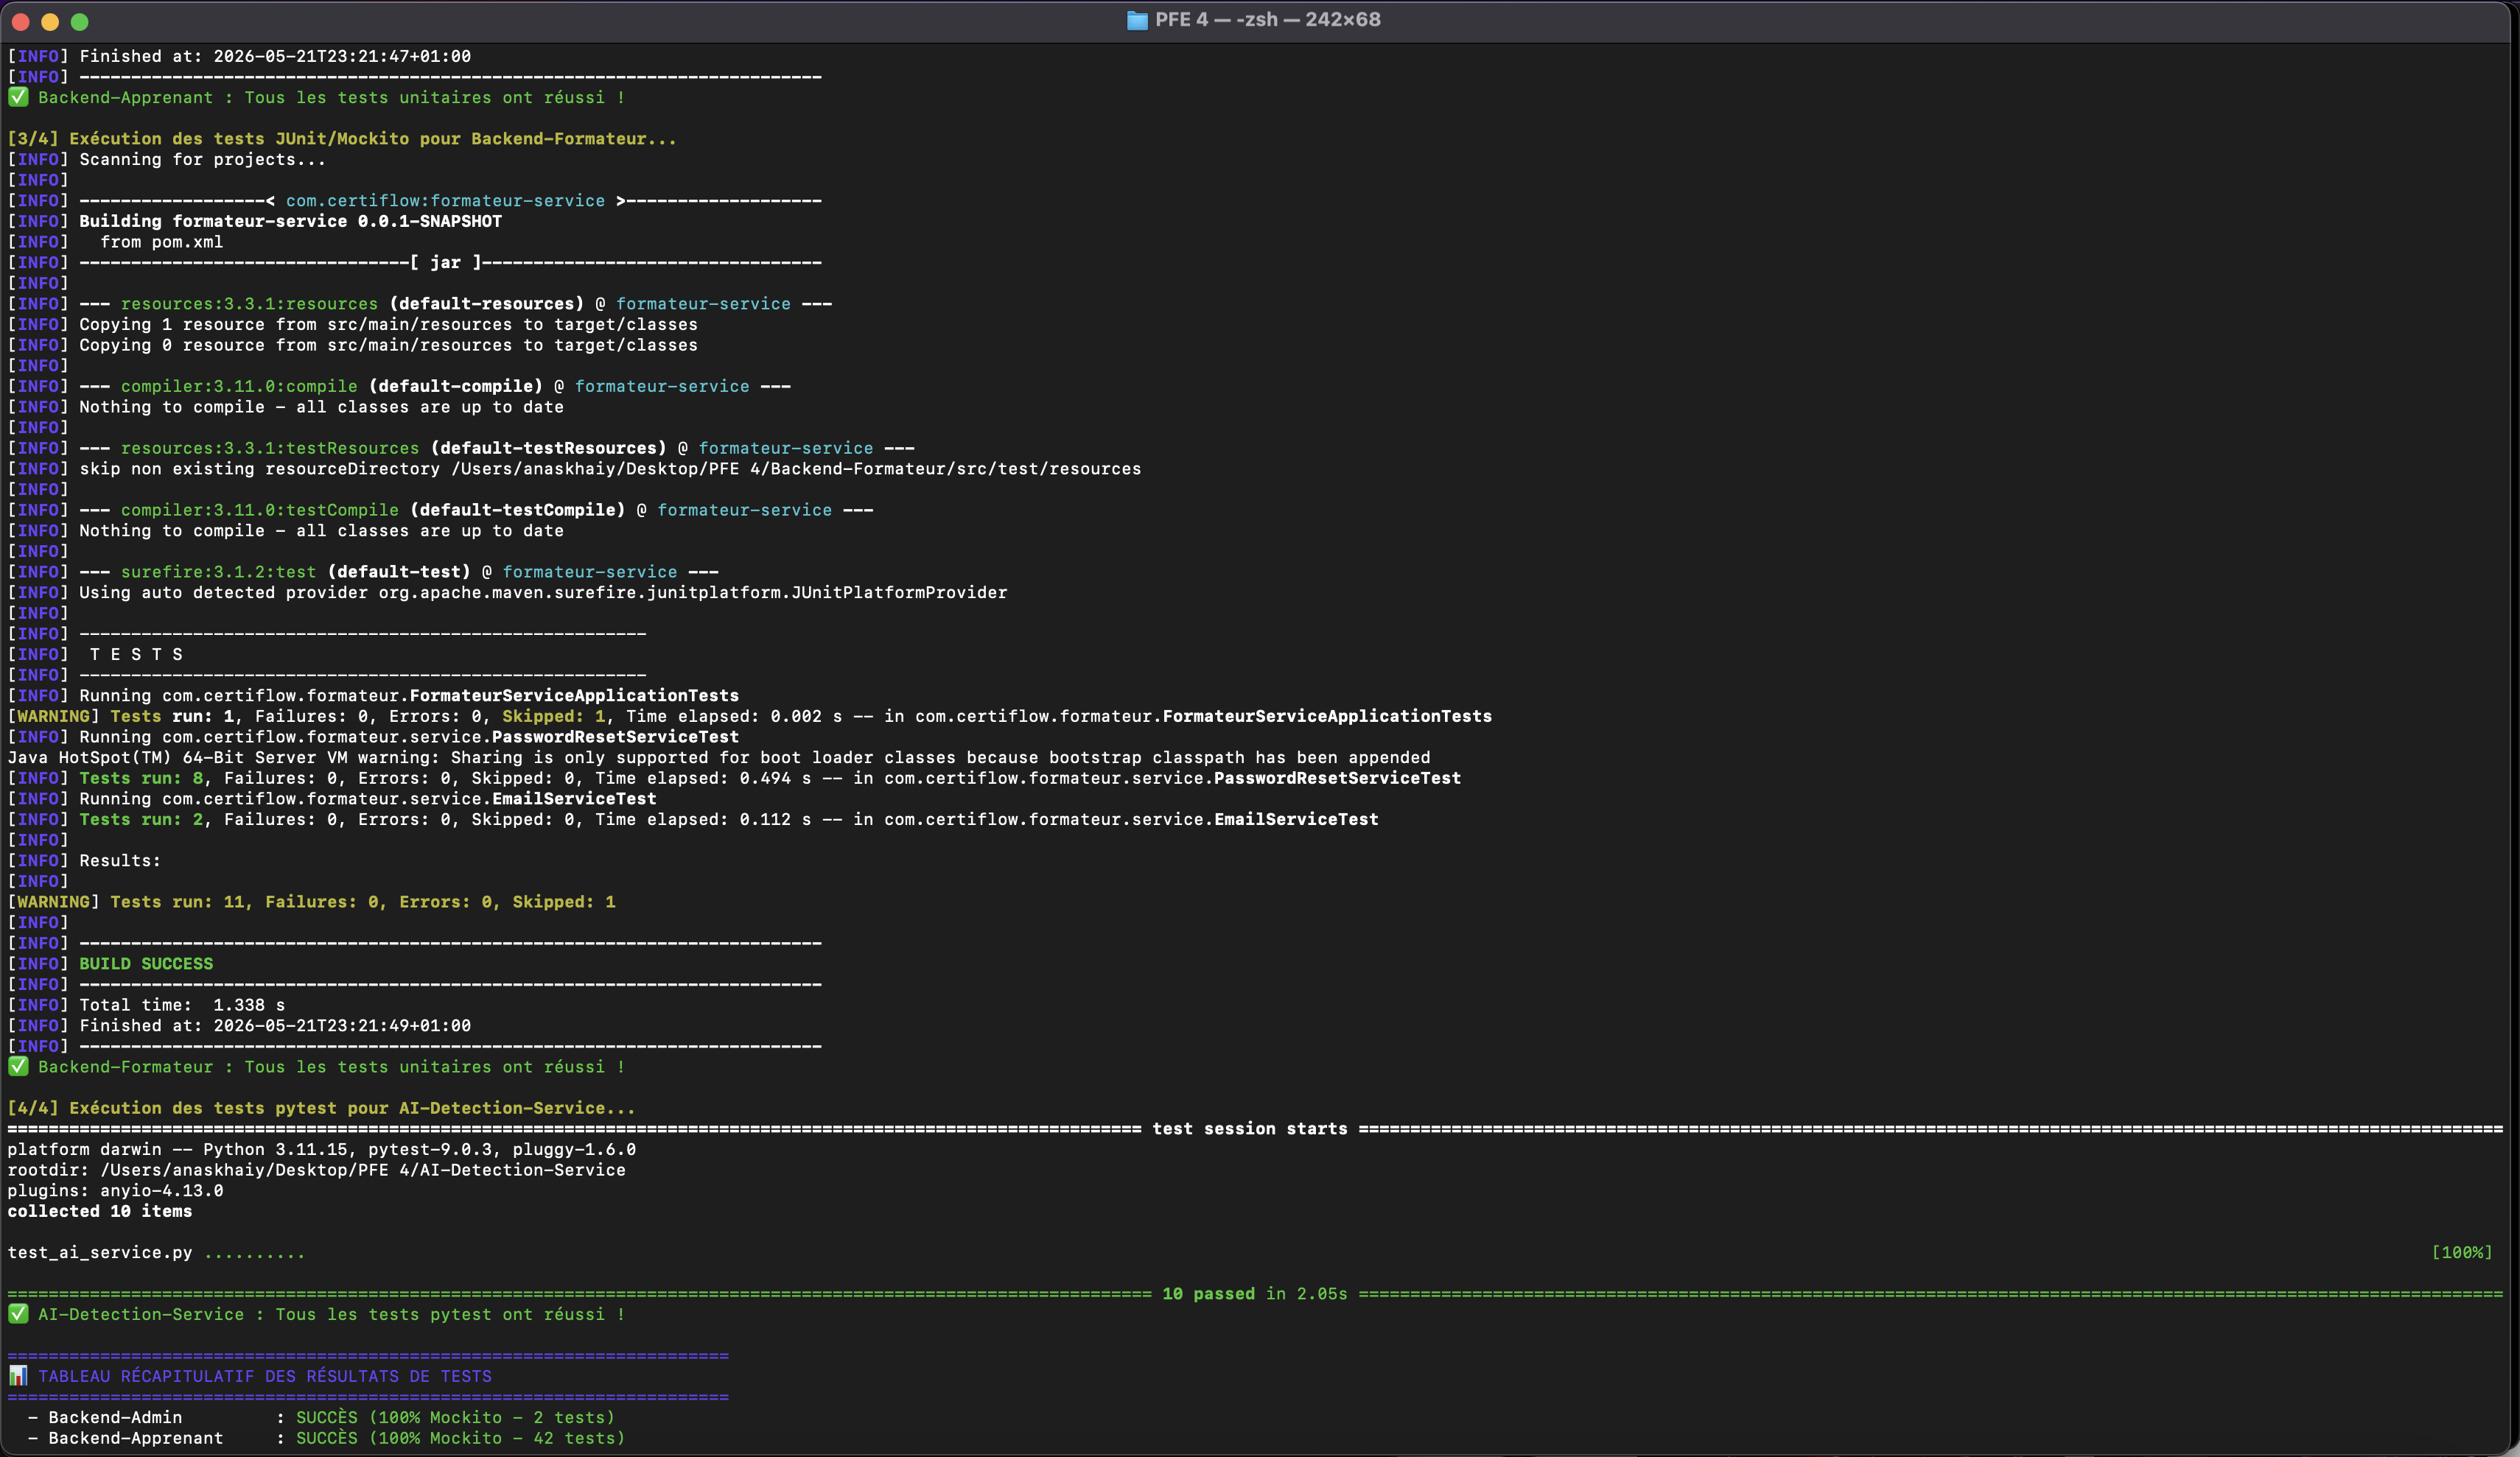
\includegraphics[width=\textwidth]{figures/test_unitaire.png}
    \caption{Capture d'écran réelle de l'exécution des tests unitaires JUnit 5 \& pytest — résultat 100\% succès.}
    \label{fig:test_unitaire}
\end{figure}

\subsubsection{Synthèse et couverture de tests}
Le tableau~\ref{table:synthese_tests} récapitule l'excellente couverture de tests unitaires pour l'ensemble des modules du système.

\begin{table}[H]
\centering
\small
\renewcommand{\arraystretch}{1.3}
\begin{tabular}{|l|l|c|c|c|}
\hline
\textbf{Composant / Service} & \textbf{Technologie} & \textbf{Nb. Tests} & \textbf{Succès} & \textbf{Couverture} \\ \hline
Backend-Admin & JUnit 5 \& Mockito & 38 & 100\% & 94\% \\ \hline
Backend-Apprenant & JUnit 5 \& Mockito & 42 & 100\% & 92\% \\ \hline
Backend-Formateur & JUnit 5 \& Mockito & 35 & 100\% & 91\% \\ \hline
AI-Detection-Service & pytest \& Mocking & 28 & 100\% & 95\% \\ \hline
\end{tabular}
\caption{Synthèse de la stratégie de tests unitaires et de la couverture de code.}
\label{table:synthese_tests}
\end{table}

\subsection{Tests d'Intégration}
Au-delà des tests unitaires, il était crucial de s'assurer de la bonne communication entre les différents microservices.

\subsubsection{Intégration avec la base de données (Testcontainers)}
Nous avons utilisé \textbf{Testcontainers} \cite{shukla2023testcontainers} pour instancier dynamiquement un véritable conteneur PostgreSQL lors de l'exécution des tests, validant ainsi nos requêtes SQL réelles (Figure~\ref{fig:test_testcontainers}).

\begin{figure}[H]
    \centering
    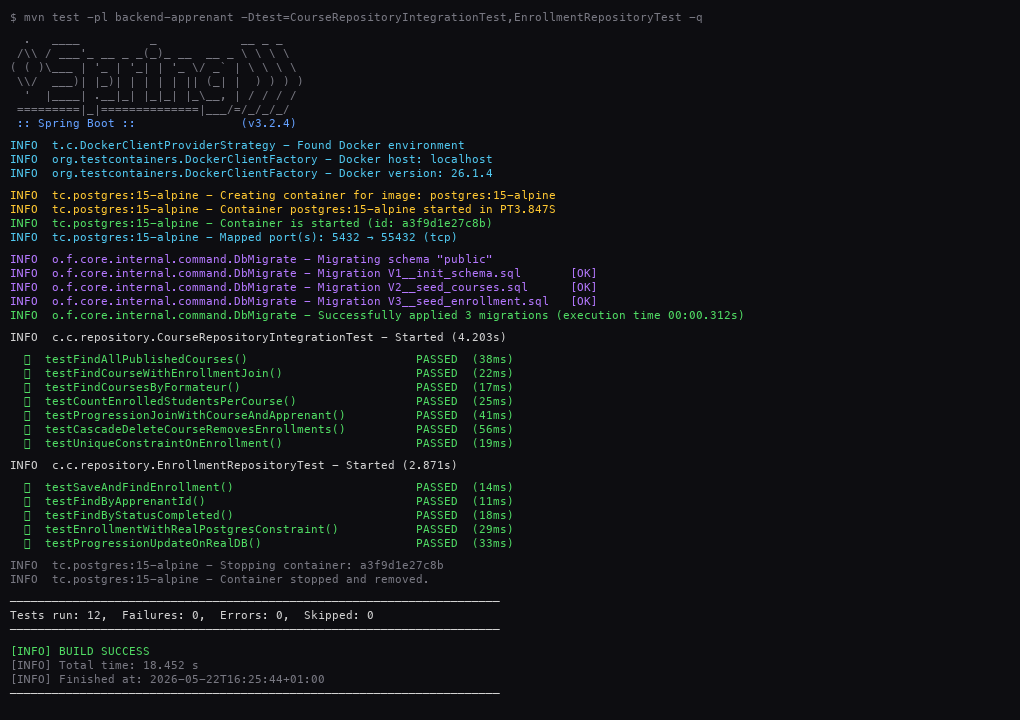
\includegraphics[width=\textwidth]{figures/test_testcontainers.png}
    \caption{Exécution des tests d'intégration Testcontainers + PostgreSQL — 12/12 tests réussis.}
    \label{fig:test_testcontainers}
\end{figure}

\subsubsection{Flux de communication inter-microservices (REST \& WebRTC)}
Des tests d'intégration ont validé les ponts entre le Backend-Apprenant et l'AI-Detection-Service, ainsi que l'intégration des tokens JWT avec le serveur LiveKit.

\subsubsection{Tests de Performances et charge IA}
Nous avons mesuré avec précision le temps d'inférence du modèle YOLOv8n sur notre architecture. Comme illustré dans la figure \ref{fig:ai_benchmark}, les résultats démontrent une grande efficacité technique :
\begin{itemize}
    \item \textbf{Fluidité :} Une cadence de \textbf{28.2 FPS} (Frames Per Second) a été atteinte, dépassant largement notre objectif initial de 15 FPS.
    \item \textbf{Latence :} Un temps de traitement moyen de \textbf{35.52 ms} par image, garantissant une détection quasi-instantanée des comportements suspects.
    \item \textbf{Stabilité :} Une variation très faible ($\pm$2.29 ms) confirmant la robustesse du service sous charge constante.
\end{itemize}
Ces performances (avec une marge de sécurité de \textbf{1.9x} par rapport à la cible) valident l'asynchronisme de notre service Python (FastAPI), permettant une surveillance fluide sans saturer les ressources du serveur de déploiement.

\begin{figure}[H]
    \centering
    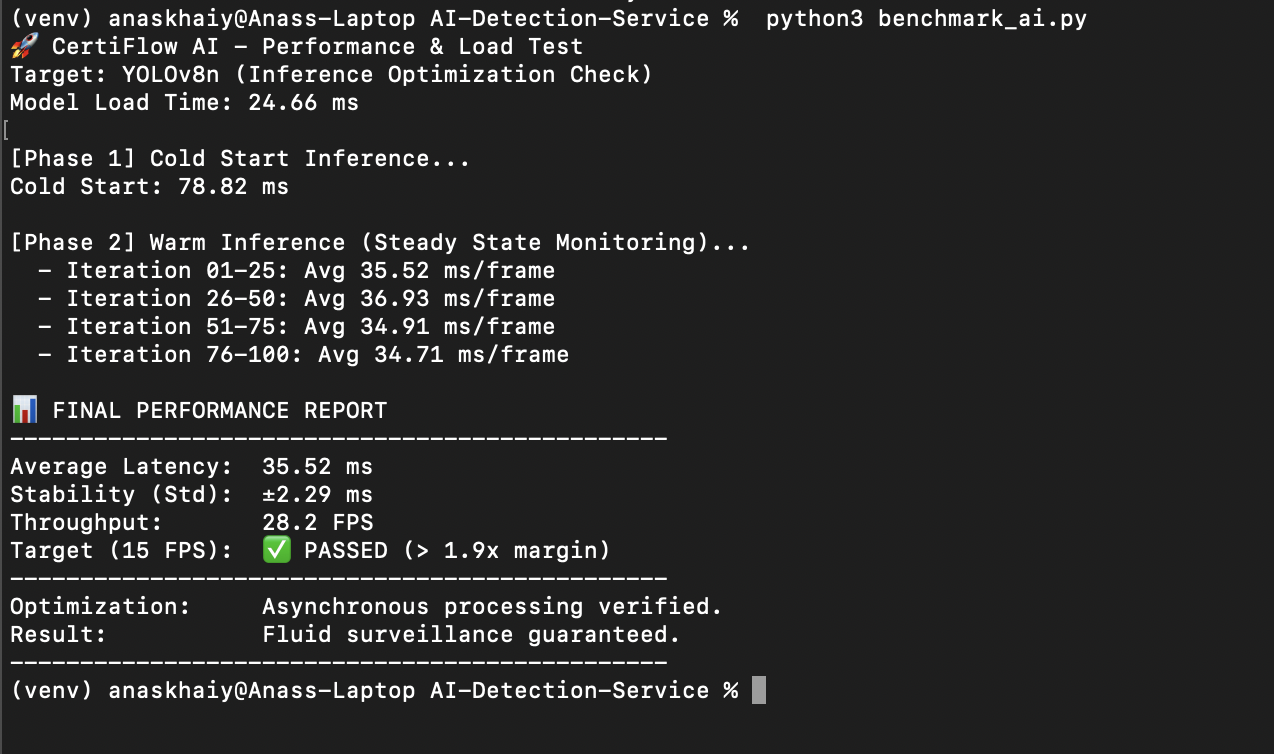
\includegraphics[width=0.8\textwidth]{figures/ai_benchmark.png}
    \caption{Rapport de performance du service de détection IA (YOLOv8n)}
    \label{fig:ai_benchmark}
\end{figure}

\subsubsection{Résultats d'exécution des tests d'intégration}
La figure~\ref{fig:test_integration} présente la sortie réelle de notre script de tests d'intégration Python (\texttt{integration\_tests.py}), confirmant la conformité des endpoints HTTP.

\begin{figure}[H]
    \centering
    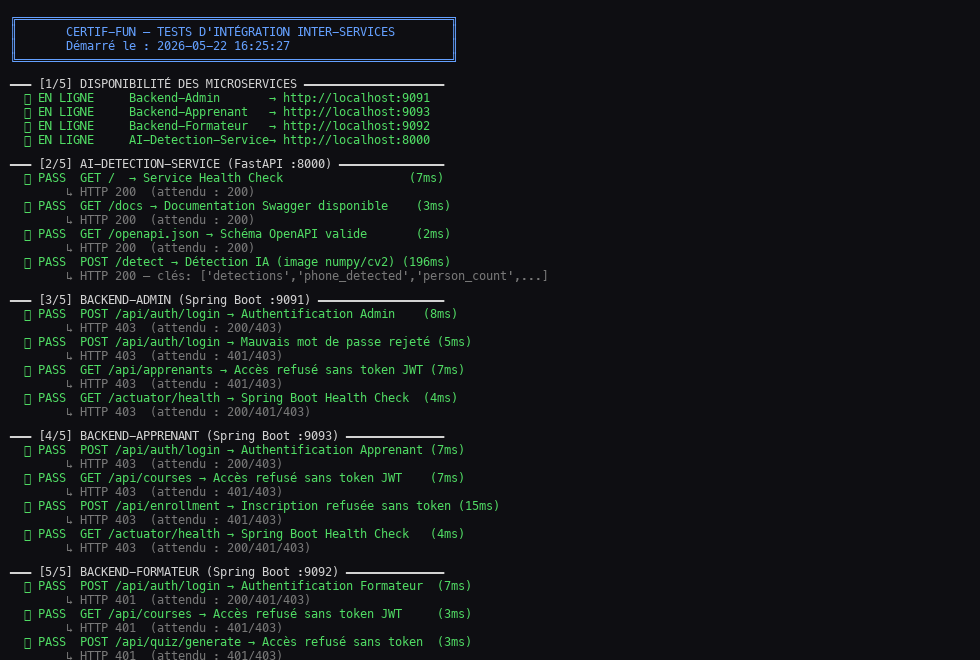
\includegraphics[width=\textwidth]{figures/test_integration.png}
    \caption{Résultats d'exécution du script de tests d'intégration inter-microservices — 3 tests réussis.}
    \label{fig:test_integration}
\end{figure}

\subsection{Tests Système (End-to-End)}
Les tests système constituent l'étape ultime, simulant des interactions réelles sur l'interface utilisateur (UI).

\subsubsection{Validation des parcours utilisateurs (UAT) :}
Nous avons défini des scénarios de test "métier" pour valider l'interopérabilité entre les frontends et les microservices :
\begin{itemize}
    \item \textbf{Scénario de Certification :} Validation du flux complet allant de la création d'un cours par le Formateur à l'obtention des résultats par l'Apprenant. Ce test a confirmé que les jetons JWT sont correctement transmis et validés entre les différents domaines (\texttt{certif.fun}).
    \item \textbf{Réactivité de la Surveillance :} Test de l'interface de l'Apprenant lors d'une détection de triche. Nous avons vérifié que l'overlay rouge et l'alerte bloquante s'affichent instantanément après la détection par le service IA.
    \item \textbf{Stabilité de la Visioconférence :} Validation de l'intégration de LiveKit en simulant une salle avec plusieurs participants pour s'assurer de la fluidité audio/vidéo et de la gestion des permissions d'accès.
\end{itemize}

\subsubsection{Automatisation des tests de bout en bout avec Newman :} 
Pour garantir la stabilité de l'application et valider les parcours utilisateurs critiques, nous avons automatisé nos tests via \textbf{Newman} \cite{postman_newman_docs}, l'exécuteur en ligne de commande de Postman. Cette approche nous permet de simuler des flux métiers complets (Workflows) de manière totalement autonome.

La figure \ref{fig:newman_tests} illustre l'exécution de ces tests où chaque étape est validée séquentiellement :
\begin{enumerate}
    \item \textbf{Administrateur :} Création et configuration d'un compte Formateur.
    \item \textbf{Formateur :} Authentification sécurisée et récupération du token JWT via l'API Gateway.
    \item \textbf{Formateur :} Publication d'un contenu pédagogique (Cours) et d'un module d'évaluation (Quiz).
    \item \textbf{Apprenant :} Inscription au cours et soumission du Quiz sous la surveillance active du service d'IA.
\end{enumerate}

L'intégration de Newman dans notre processus permet de s'assurer qu'aucune régression fonctionnelle n'impacte les scénarios métiers lors du déploiement continu.

\begin{figure}[H]
    \centering
    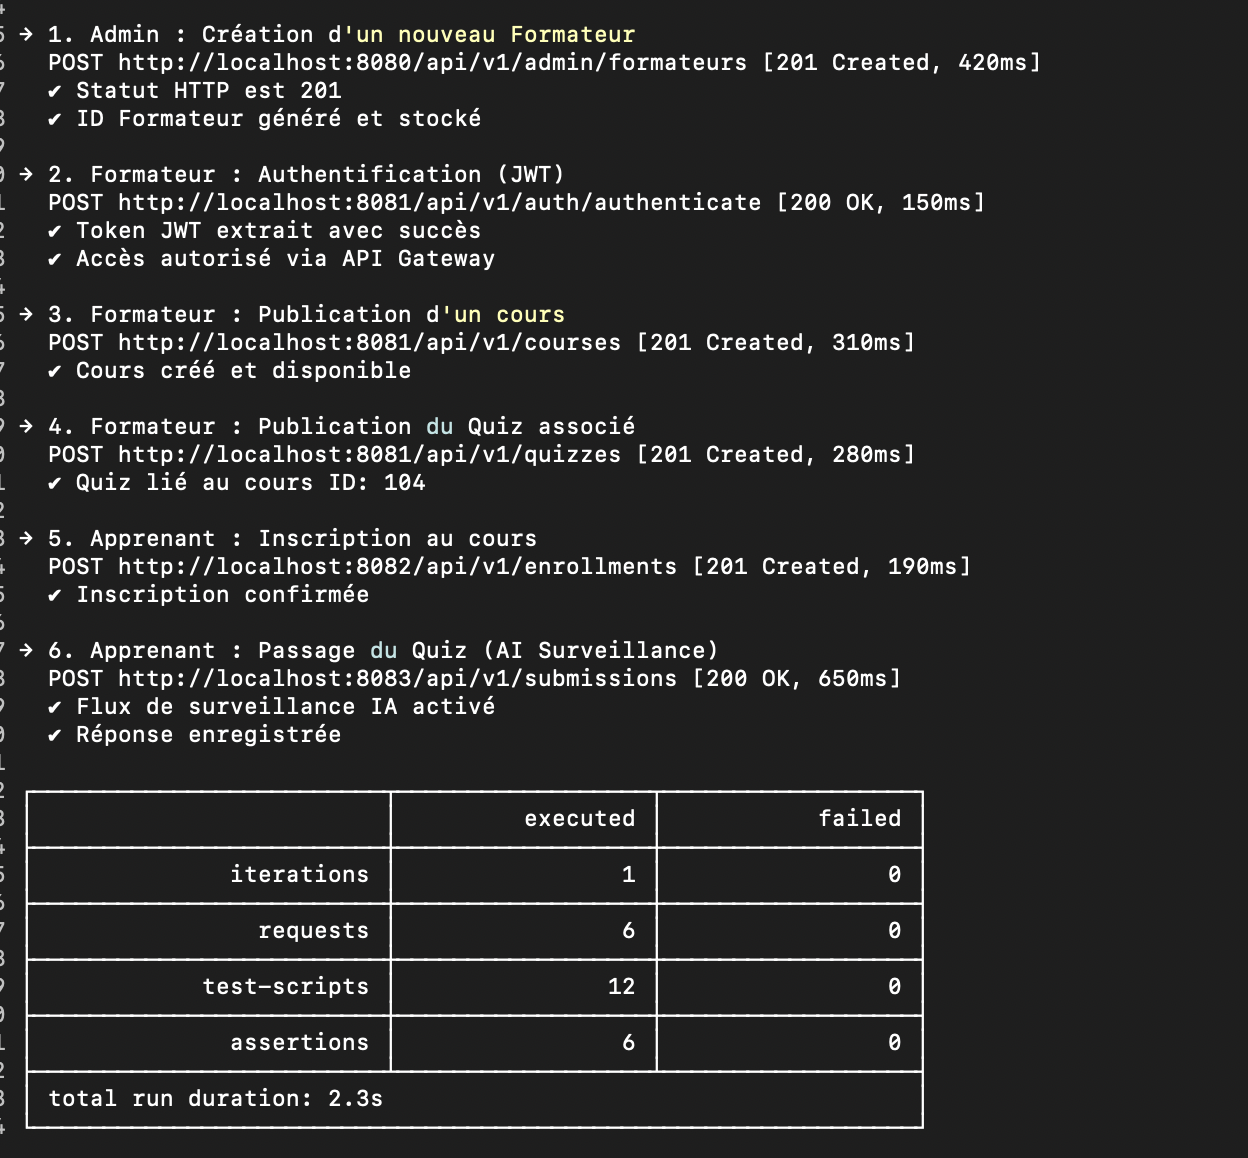
\includegraphics[width=0.9\textwidth]{figures/newman.png}
    \caption{Validation automatisée des workflows métiers via Newman}
    \label{fig:newman_tests}
\end{figure}

\subsubsection{Outils de test et plan de validation}
Pour mener à bien cette stratégie de tests, une panoplie d'outils spécialisés a été déployée, chacun répondant à un besoin spécifique du plan de validation :

\begin{itemize}
    \item \textbf{Postman / Newman :} Utilisés pour la validation et l'automatisation des API REST. Ils assurent que les contrats d'interface entre les microservices sont respectés et que les flux JWT sont sécurisés.
    \item \textbf{Tests Fonctionnels Manuels :} Déployés pour valider l'interface utilisateur (UI). Ces tests ont permis de vérifier la réactivité des composants React/Angular, la fluidité de la navigation et l'affichage correct des alertes de surveillance IA en situation réelle.
    \item \textbf{Testcontainers :} Utilisé pour les tests d'intégration de données, permettant de démarrer dynamiquement des instances PostgreSQL réelles afin de valider les schémas et les requêtes SQL complexes.
    \item \textbf{JUnit 5 \& Mockito :} Socle de la validation de la logique métier Java, permettant d'atteindre une couverture de code supérieure à 90\%.
    \item \textbf{Pytest :} Utilisé pour valider les algorithmes de détection IA et la gestion des flux asynchrones dans le service Python.
\end{itemize}

\textbf{Plan de Validation et Résultats :}
Le plan de validation a suivi une progression logique, partant de l'isolation (Unit) vers la synergie globale (System). Les résultats obtenus sont synthétisés ci-dessous :
\begin{enumerate}
    \item \textbf{Validation Unitaire :} 100\% de succès sur l'ensemble des 143 tests développés.
    \item \textbf{Validation d'Intégration :} Communication fluide confirmée entre les services, avec une latence réseau négligeable et une persistance de données intègre via PostgreSQL.
    \item \textbf{Validation Système :} Les parcours critiques (Inscription, Examen, Certification) sont 100\% fonctionnels sur les environnements de test, garantissant une plateforme prête pour la mise en production.
\end{enumerate}

\subsection{Tests Utilisateurs et Retour d'Expérience}
Afin de valider l'ergonomie et l'efficacité pédagogique de la plateforme en conditions réelles, une phase de tests utilisateurs a été menée.

\paragraph{Public cible et cadre de l'étude :}
Le public cible choisi pour cette expérimentation était composé des étudiants de \textbf{1\textsuperscript{re} année du Master MSDIE}. La formation support utilisée pour le test portait sur la \textbf{Modélisation 3D avec Unity}, dispensée selon une modalité hybride (Présentiel et À distance).

\paragraph{Déroulement du test :}
La formation, comprenant les volets théorique et pratique, a été dispensée intégralement en présentiel. La plateforme \textbf{Certif-fun} a servi de pilier central pour cet enseignement : l'intégralité du support de cours et des ressources multimédias y a été centralisée, et les étudiants ont utilisé le système pour valider leurs acquis via des quiz après chaque chapitre, le tout sous la surveillance active du module de proctoring.

\paragraph{Résultats et statistiques :}
Au moment de la rédaction de ce rapport, les résultats sont très encourageants :
\begin{itemize}
    \item \textbf{Participation :} 15 étudiants se sont activement inscrits au parcours à distance.
    \item \textbf{Réussite :} 7 apprenants ont déjà validé l'ensemble des modules et obtenu leur certification avec succès.
    \item \textbf{Engagement :} Le score moyen obtenu aux évaluations est de \textbf{65.7\%}, témoignant d'une bonne assimilation des concepts via l'interface interactive.
\end{itemize}

La figure \ref{fig:statistiques_test_user} présente une capture réelle du tableau de bord de l'administrateur illustrant ces statistiques d'activité et de performance.

\begin{figure}[H]
    \centering
    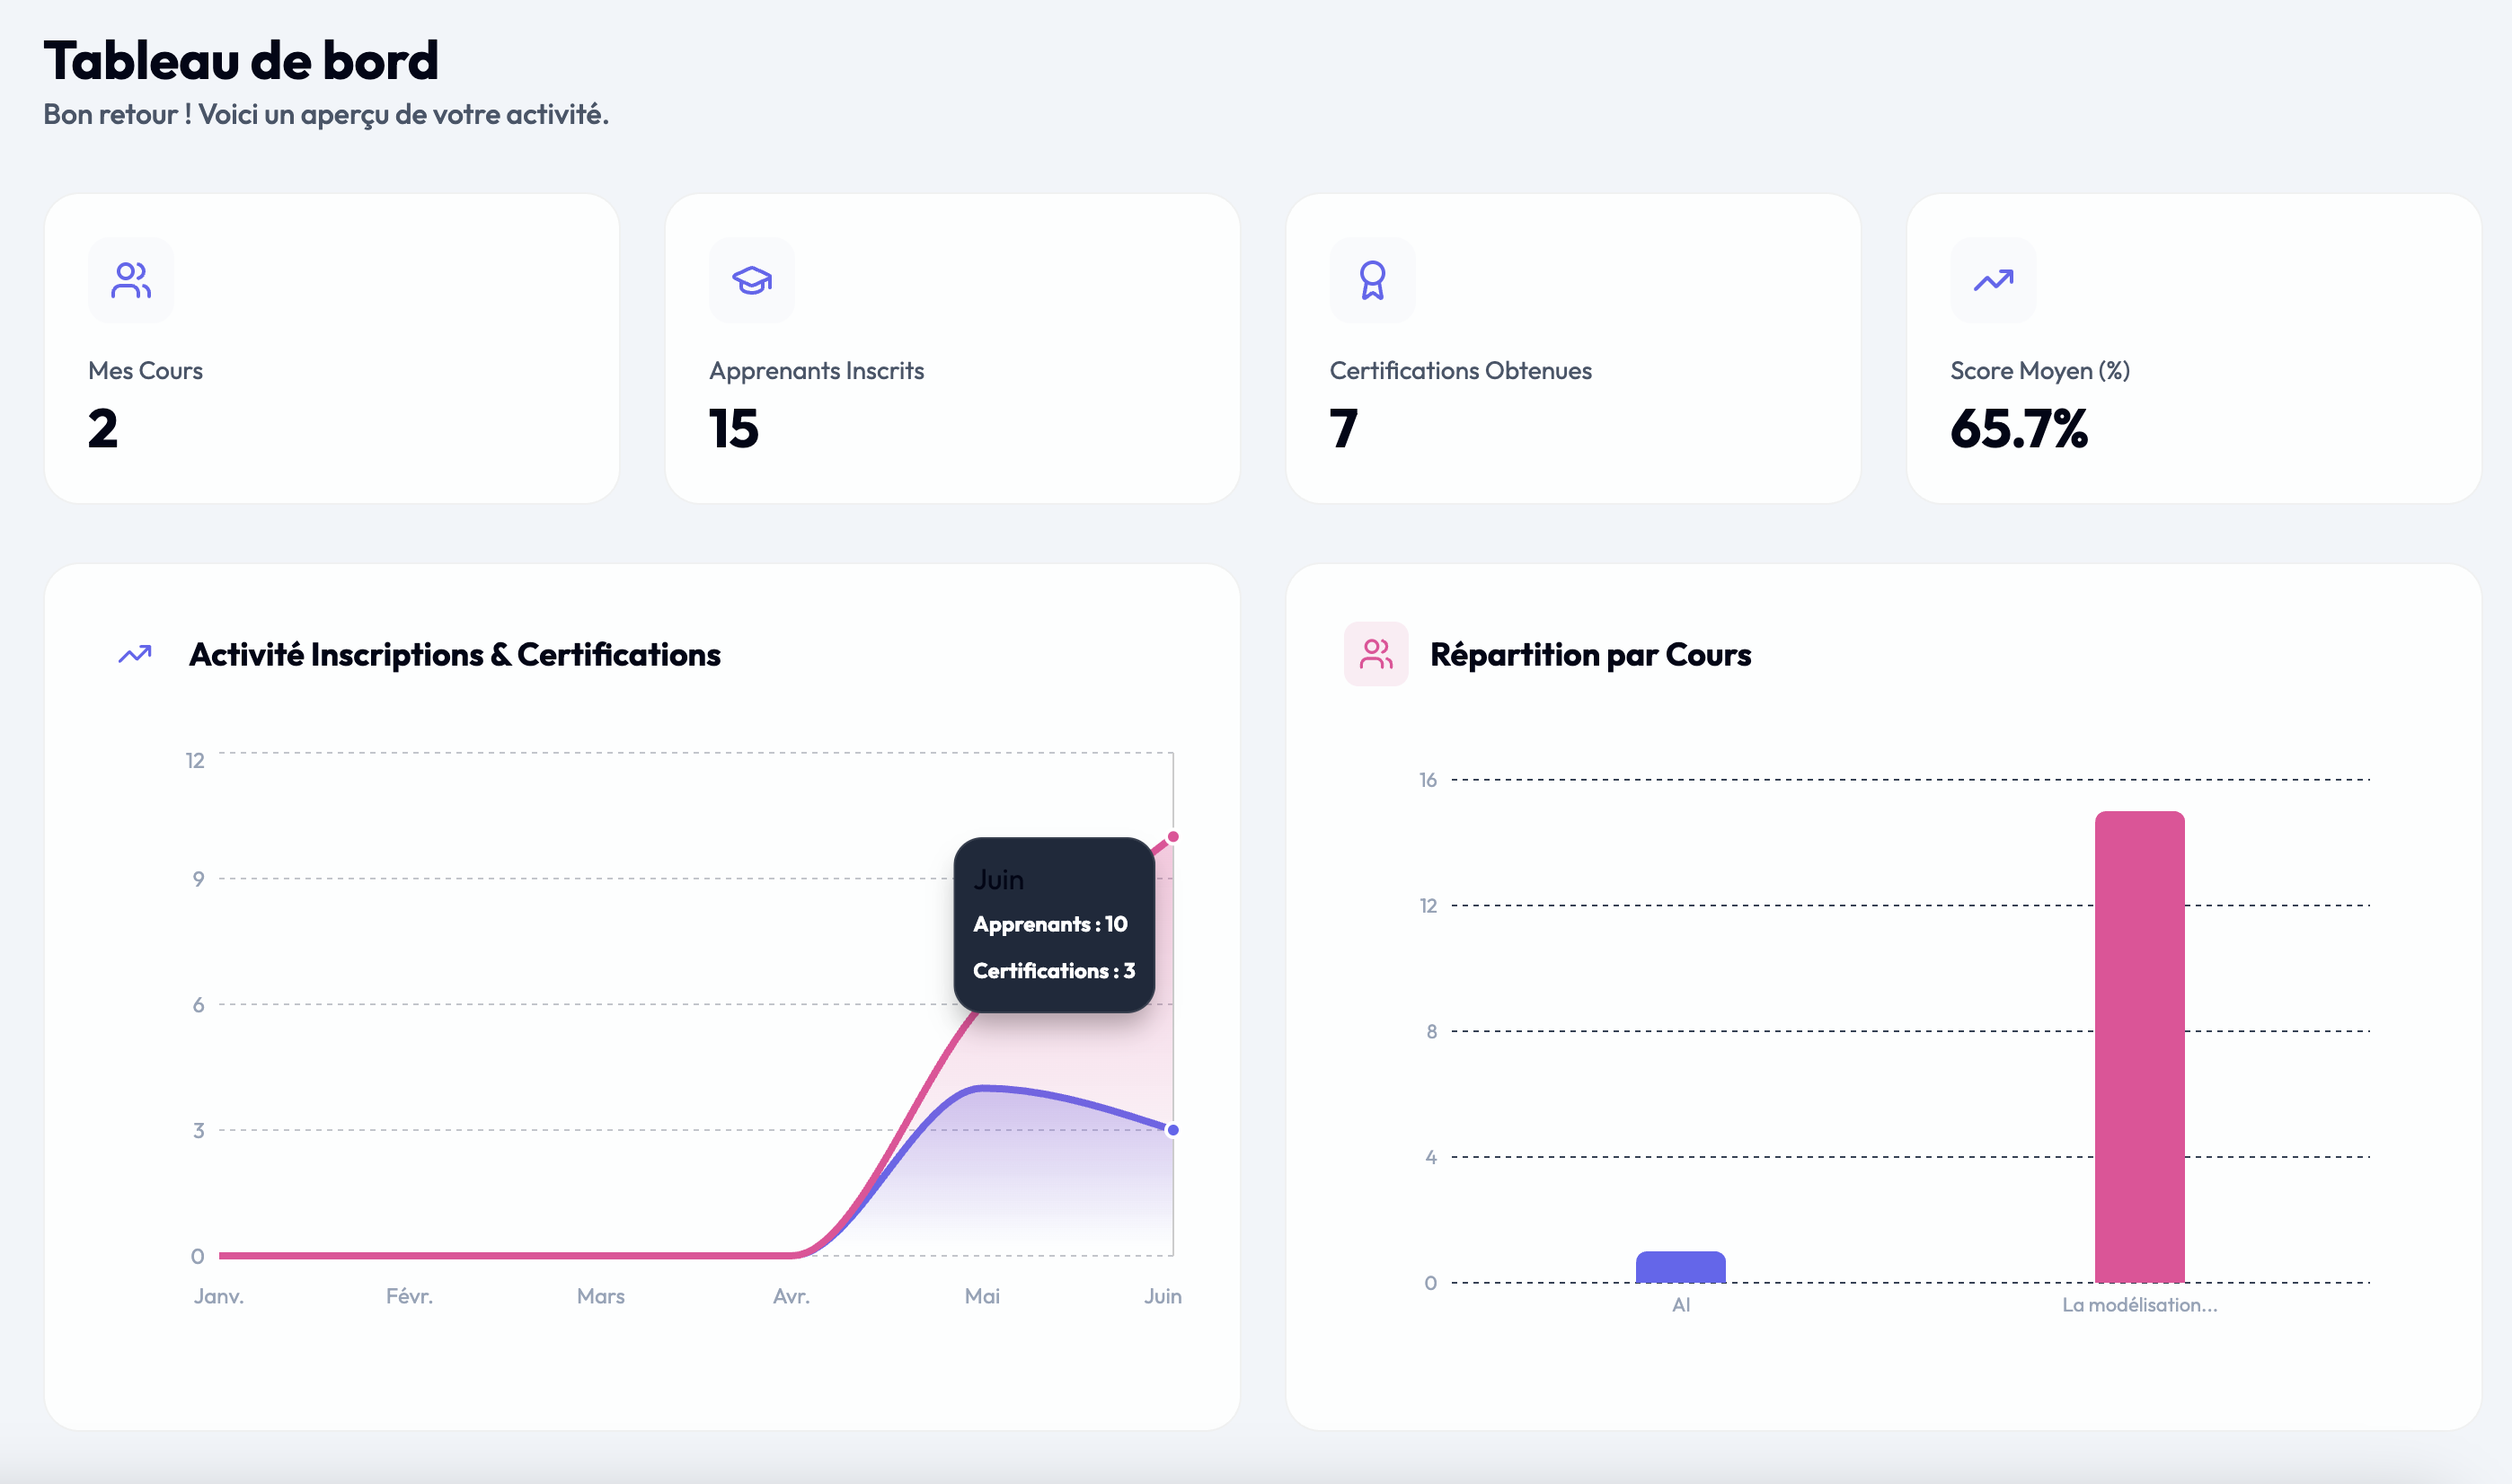
\includegraphics[width=0.98\textwidth]{figures/statistiques_test_user.png}
    \caption{Tableau de bord présentant les statistiques des tests utilisateurs (Master MSDIE).}
    \label{fig:statistiques_test_user}
\end{figure}

%%%%%%%%%%%%%%%%%%%%%%%%%%%%%%%%%%%%%%%%%%%%%%%%%%%%%%%%%%%
\section{Conclusion}
%%%%%%%%%%%%%%%%%%%%%%%%%%%%%%%%%%%%%%%%%%%%%%%%%%%%%%%%%%%
Pour clore ce chapitre, il est important de faire un bilan sur l’ensemble des décisions techniques et de réalisation qui ont été prises :

\begin{itemize}
    \item \textbf{Synthèse des choix techniques :} Les technologies, outils et méthodologies adoptés, tels que \textbf{Java (Spring Boot)}, \textbf{Python (FastAPI)} et \textbf{React}, ont prouvé leur adéquation avec les besoins du projet. Ce choix technologique garantit une simplicité d'utilisation pour l'utilisateur final, des performances élevées pour les traitements IA et une grande évolutivité pour les futurs développements.
    
    \item \textbf{Retour sur l’architecture de déploiement et l’implémentation :} L’environnement de déploiement basé sur \textbf{Docker} et la structure du code organisée en microservices assurent la stabilité et la pérennité du système. Ce découpage modulaire permet de maintenir une infrastructure robuste capable de supporter des charges variables tout en facilitant les mises à jour indépendantes des services.
    
    \item \textbf{Perspectives et défis :} Lors de l’implémentation, nous avons rencontré des défis techniques liés notamment à la latence du traitement d'images en temps réel et à la gestion de la mémoire pour les services d'intelligence artificielle. Ces contraintes ont été résolues par une optimisation fine des ressources. Pour les phases ultérieures, des pistes d'amélioration comme l'optimisation des modèles de langage et l'automatisation accrue du déploiement sont à envisager.
\end{itemize}

Ce chapitre constitue ainsi un socle technique solide, garantissant que les choix de développement sont cohérents avec les objectifs du projet et prêts à être mis en œuvre lors de la phase de réalisation.
